\documentclass[11pt]{article}
\usepackage[margin=1in]{geometry}
\usepackage{booktabs}
\usepackage{graphicx}
\usepackage{amsmath}
\usepackage{caption}
\captionsetup{font=small,skip=6pt}

\title{Screening deployed arms by pseudo-outcome risk share\\
\large A large-batch proof of concept}
\author{}
\date{}

\begin{document}
\maketitle

\section{What was run}

Four fixed linear scorecards compete on successive batches.
The reward is negative batch mean squared error.
Excess on a round is the gap between the served scorecard and the best scorecard on that batch.
The FSDS weight of scorecard \(k\) is the held-out residual variance of its doubly robust pseudo-outcome, divided by the sum of those residuals across the four scorecards.
The pseudo-outcome compares a fixed reference window (the first six batches) with the latest six batches.
The share is refreshed every eight rounds from round 16.
It is computed from every scorecard's prediction on the logged batch, so it does not require that the scorecard was served.

The index is the usual UCB, discounted UCB, or Thompson draw, minus a tax \(\eta\sigma w_k\).
Here \(\sigma\) is the standard deviation of the four arm rewards on the reference window, and \(\eta\in\{0.5,1,2\}\).
An absolute penalty \(\lambda=5\), not scaled by \(\sigma\), is reported as a check.
No rule uses \(\lambda=20\) or \(\lambda=40\).
Epsilon-greedy at \(5\%\), \(10\%\), and \(15\%\) is the uniform-exploration comparator, and one extra rule puts the \(\eta=1\) tax on the \(10\%\) rule.

Each batch has \(200\) rows.
There are \(80\) rounds.
A gradual path holds the mixing weight at \(0\) through round \(20\) and then ramps to \(1\).
A drastic path jumps at round \(40\).
Post-shift totals use rounds whose mixing weight is at least \(1/2\).
Early totals use rounds whose mixing weight is exactly \(0\).
The ramp in between is reported separately.
Four seeds, \(20261018\) through \(20261021\), are averaged.
Parentheses in the tables are the seed standard deviation.

The covariate pools all have at least \(10{,}000\) rows, or are synthetic of that size.
Columns are standardized.
\begin{center}
\begin{tabular}{lll}
\toprule
Pool & Rows used & Columns \\
\midrule
Gaussian & \(20{,}000\) & \(30\) \\
Gaussian & \(20{,}000\) & \(12\) \\
Student-\(t_5\) & \(20{,}000\) & \(30\) \\
AR(1) Gaussian, correlation \(0.6\) & \(20{,}000\) & \(30\) \\
California housing & \(20{,}640\) & \(8\) \\
Covertype, draw from \(581{,}012\) & \(30{,}000\) & \(54\) \\
\bottomrule
\end{tabular}
\end{center}
Real matrices supply covariates only.
The label is the synthetic shift: relocation of a linear block, a sign flip, a dying block, a nonlinear add-on, or growing noise.
The headline number below is the median, across the six pools, of the four-seed mean.
California's nonlinear add-on produces a very large squared term, so a raw mean would follow that one pool.

A second horse-race replaces scorecards by four linear policies on a horizon of four steps, with \(200\) episodes in each round.
The same residual share is computed from each policy's scalar self-score.
Three monitors are compared: an oracle that sees every policy's return, an on-policy log of the served policy only, and a least-squares reward fit that imagines the unserved policies.

\section{What the share is doing}

On a gradual relocation the share does not chase the scorecard whose predictions move the most.
It chases the scorecard that has stopped explaining the outcome.

\begin{figure}[ht]
\centering
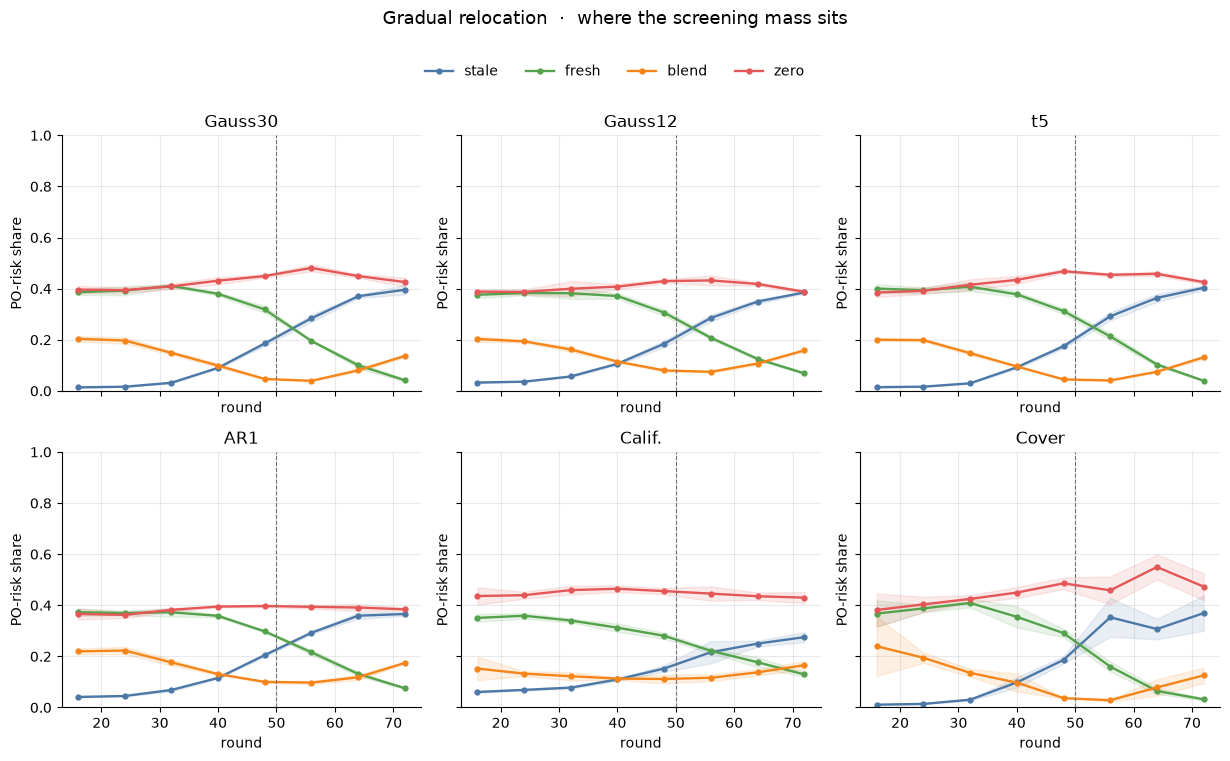
\includegraphics[width=\textwidth]{figures/shares_gradual_relocate.png}
\caption{PO-risk shares on a gradual relocation.
Before the ramp, the fresh block and the zero score hold the mass, and the stale block, which still carries the signal, sits near zero.
After the mixing weight passes \(1/2\) (dashed line), the fresh share falls and the stale share rises to meet the zero score.
The same crossing appears on all six pools.
California, with only eight columns, separates more slowly.}
\end{figure}

Before the move, \(y\) is the stale block.
A regression of the pseudo-outcome on that score absorbs the contrast, so its residual share is small.
The fresh block is orthogonal to \(y\), and the zero score has nothing to project onto, so those two residuals take the share.
After the move, \(y\) lives on the fresh block.
The fresh residual collapses and the stale residual inflates, because the current-window leftover is now orthogonal to the stale score.
The zero score never explains \(y\), so it keeps a large share throughout.
Post-shift means on the Gaussian \(d=30\) pool are about \(0.35\) on the stale block, \(0.11\) on the fresh block, \(0.09\) on the blend, and \(0.45\) on zero.
Covertype is sharper: about \(0.34\), \(0.09\), \(0.08\), and \(0.49\).

The tax \(-\eta\sigma w_k\) is therefore a screen on currently unexplained scores.
An arm that moves with the world sheds the tax.
An arm that moves against the world, or that never carried the signal, keeps it.
That is why a penalty on the raw change in the arm's own prediction would be the wrong instrument: the fresh card's fitted mean moves the most, and that movement is the signal.

While the mixing weight is still zero, UCB and UCB with \(\eta\in\{1,2\}\) have the same early excess (median \(16.1\) on gradual relocation).
The relevant arm already wins the reward index, and the tax on the irrelevant arms does not change the argmax.
Epsilon-greedy pays immediately: its early median is \(19.9\) at \(10\%\).

\section{Where the tax earns its keep}

\begin{figure}[ht]
\centering
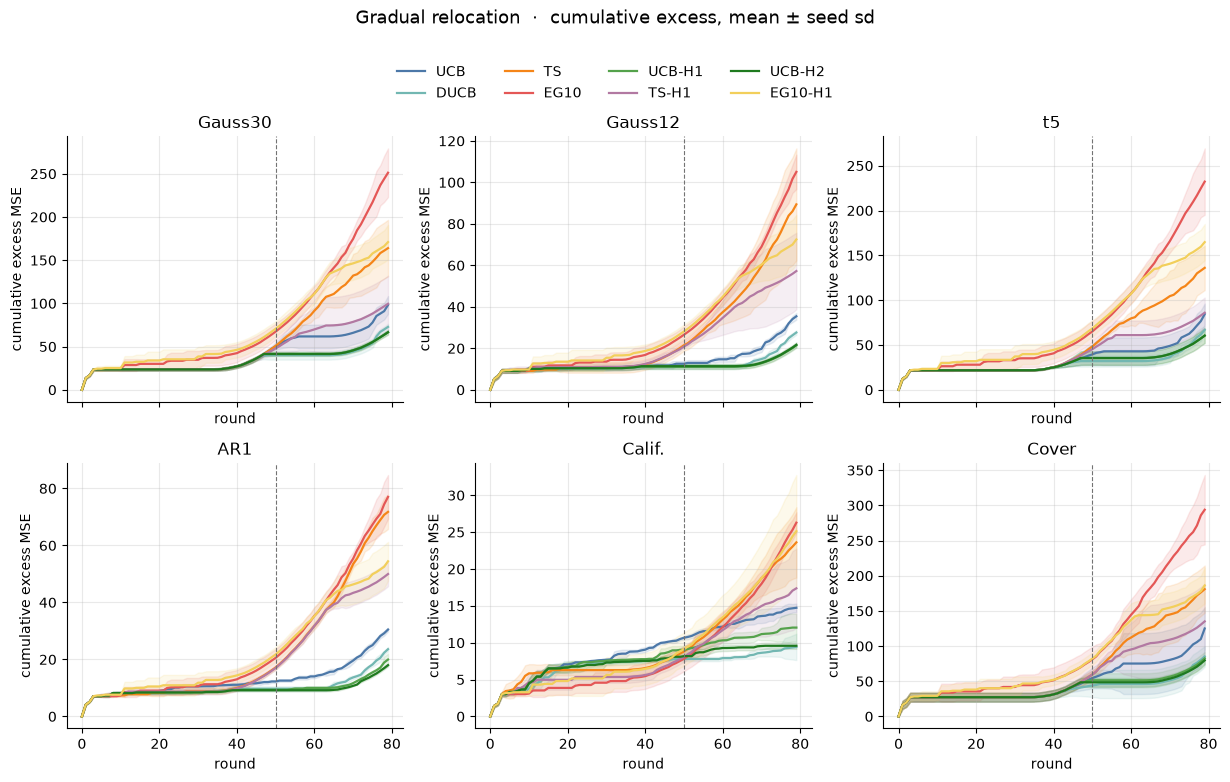
\includegraphics[width=\textwidth]{figures/cum_gradual_relocate.png}
\caption{Cumulative excess on a gradual relocation.
UCB with \(\eta=1\) or \(2\) stays flat after the dashed line.
Epsilon-greedy at \(10\%\), with or without the tax, keeps accumulating.
Thompson sampling without the tax tracks the exploring rules; with \(\eta=1\) it moves toward UCB.}
\end{figure}

\begin{figure}[ht]
\centering
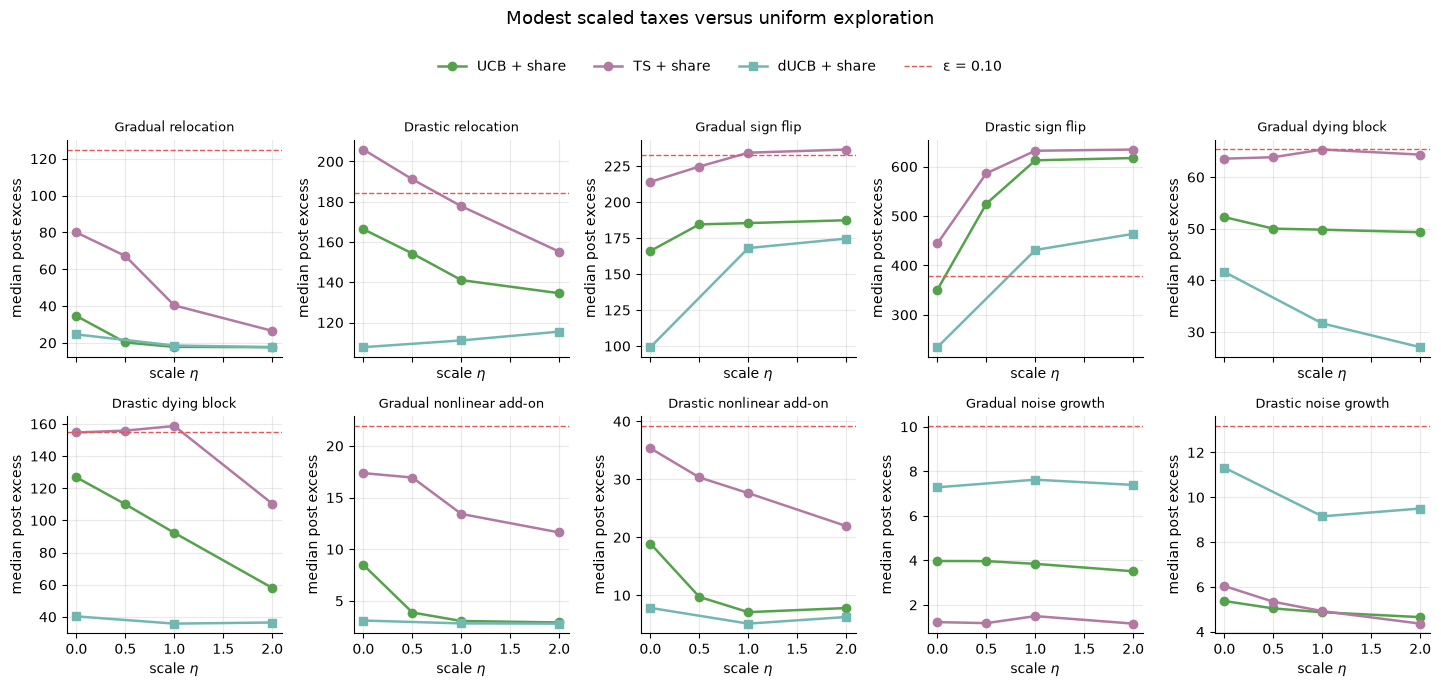
\includegraphics[width=\textwidth]{figures/eta_profile.png}
\caption{Median post-shift excess against the scale \(\eta\).
The dashed line is epsilon-greedy at \(10\%\).
Relocation, a dying block, and a nonlinear add-on slope down for UCB.
A sign flip slopes up: the tax is the wrong sensor there.
Noise growth is already small for Thompson sampling, and discounting sits above UCB because the best card never changes.}
\end{figure}

Three regimes show up on every pool.

\paragraph{The signal changes subspace.}
Gradual relocation, the nonlinear add-on, and a dying block are this case.
The median post-shift excess on gradual relocation is \(34.6\) for UCB, \(24.6\) for discounted UCB, \(80.0\) for Thompson sampling, and \(125.0\) for epsilon-greedy at \(10\%\).
UCB with \(\eta=2\) and discounted UCB with \(\eta=2\) both sit at \(17.6\).
That removes \(49\%\) of the UCB total and \(86\%\) of the epsilon-greedy total, and it is lower than discounting alone on all six pools.
The same ordering holds at \(\eta=1\) (\(17.8\)).
Epsilon at \(5\%\) is still \(100.6\), and epsilon at \(15\%\) is \(82.6\): a larger uniform share spends more whole batches on a wrong scorecard and does not locate the fresh block any faster.
On the nonlinear add-on the best median is discounted UCB at \(\eta=2\), \(2.80\), against \(8.48\) for UCB and \(21.9\) for epsilon at \(10\%\).
On a gradual death the same rule is \(27.1\), against \(41.6\) for discounting alone and \(52.2\) for UCB.

A drastic relocation is the boundary inside this regime.
Plain discounted UCB is best, at \(107.7\).
Adding \(\eta=1\) moves it to \(111.1\), and \(\eta=2\) to \(115.5\).
The share still separates (fresh near \(0.09\), stale near \(0.32\)), and the tax still beats plain UCB (\(166.3\) to \(134.6\) at \(\eta=2\)).
Once the index is already discounting, a jump of this size is carried by the reward, and the extra tax does not pay.

\paragraph{The signal flips sign.}
A within-window least squares absorbs the sign into the two window-specific slopes.
The residual then cannot prefer the flipped card.
On a drastic flip the two signed scores each hold about \(0.03\) of the share and the zero score holds about \(0.90\).
They are tied, so the tax has nothing to say about which sign is current.
What it does say is to avoid zero.
After the flip, predicting zero is the hedge: its mean squared error is on the order of the signal variance, while predicting the wrong sign is on the order of four times that variance.
UCB without the tax retreats toward zero.
UCB with \(\eta=1\) is forbidden from that retreat and stays on the stale sign.
The median post-shift excess goes from \(351\) for UCB and \(235\) for discounted UCB to \(613\) for UCB at \(\eta=1\), and from \(235\) to \(431\) for discounted UCB at \(\eta=1\).
The shut-off is visible in the share itself, before any regret is computed.
If one null score holds most of the mass and the remaining scores are tied, set \(\eta=0\) and discount the reward.
Discounting wins both the gradual flip (\(99.2\)) and the drastic flip (\(234.6\)).
It wins by hedging toward zero, not by discovering the flipped card: that card's pre-flip mean is terrible and it is almost never pulled.

\paragraph{Only the noise scale changes.}
The linear score stays correct, and its share stays small, about \(0.10\) to \(0.18\).
The tax lands on zero and on the irrelevant block.
Discounting discards a history that is still valid, so discounted UCB is worse than UCB (\(7.28\) against \(3.97\) on the gradual path, \(11.3\) against \(5.37\) on the drastic path).
Thompson sampling already concentrates on the unchanged arm.
A small tax on top of it is the best rule in the grid: absolute \(\lambda=5\) has median \(0.90\) (gradual) and \(4.21\) (drastic), with Thompson at \(\eta=2\) close behind at \(1.16\) and \(4.36\).

\section{How large the effect is}

The median is a summary. The claim that the tax works has to survive two stricter checks: it has to appear on each pool, and the gap has to be larger than the seed standard deviation of either rule. Table~\ref{tab:effect:reloc} and Table~\ref{tab:effect:clear} are those checks. Every raw mean, for every rule and every pool, is in the appendix.

\paragraph{Gradual relocation is the clean effect.}
UCB at \(\eta=2\) cuts the post-shift excess on all six pools, by \(46\%\) to \(65\%\):
Gaussian \(d=30\) from \(50.6\) to \(25.1\),
Gaussian \(d=12\) from \(22.9\) to \(10.3\),
Student-\(t_5\) from \(46.3\) to \(25.0\),
AR(1) from \(18.2\) to \(8.8\),
California housing from \(4.2\) to \(1.5\),
Covertype from \(73.1\) to \(31.2\).
On each pool the gap exceeds the larger seed standard deviation, and the taxed seed standard deviation is itself smaller (Covertype falls from \(20.7\) to \(1.2\)).
Against discounted UCB the same gap clears the seed noise on five pools.
California is the exception: discounting alone is already \(1.65\) with seed sd \(1.50\), and the tax moves the point estimate to \(1.49\).
That pool has only eight columns, so the two blocks are short and the share separates more slowly.
Against \(\varepsilon=0.10\) the removed fraction is \(85\%\) to \(92\%\) on every pool, and the gap is several times the seed noise.

The hit rate explains what kind of improvement this is.
On the four large synthetic pools, UCB's post-shift hit rate is about \(0.38\) to \(0.44\), and the taxed rule is about \(0.47\) to \(0.51\).
Excess falls by half while the fraction of rounds on the unique best card rises by only about ten points.
The tax is not finding a hidden optimum on every round.
It is refusing the stale card and the zero card.
The blend, which is close to the fresh block during the ramp, absorbs many of the remaining rounds, so the excess of those rounds is small.
Epsilon-greedy's hit rate on the same pools is about \(0.03\).
It almost never serves the best card after the shift, which is why its excess is \(57\) to \(217\).

The early window, mixing weight exactly zero, does not pay for this.
UCB and UCB at \(\eta=2\) have the same early total on Gaussian \(d=30\) (\(23.5\)), Gaussian \(d=12\) (\(10.4\)), Student-\(t_5\) (\(21.8\)), and Covertype (\(27.3\)).
AR(1) moves from \(8.95\) to \(8.43\), and California from \(7.06\) to \(6.62\).
Epsilon at \(10\%\) is already higher on five of the six pools before anything moves.

\paragraph{Where the same bar is cleared, and where it is not.}
Table~\ref{tab:effect:clear} counts a pool only when the candidate beats the baseline by more than the larger seed standard deviation.
Growing noise, with Thompson at \(\eta=2\), clears UCB on all six gradual pools and discounted UCB on all six.
The best card never changed, the share stays on the irrelevant scores, and the tax is a small push on top of a posterior that was already in the right place.
A drastic relocation clears UCB on five pools and discounted UCB on none.
The share still points at the stale block, and that is enough to beat a rule that keeps the whole history.
It is not enough to beat a rule that is already forgetting that history.
A sign flip clears nobody who matters.
Taxed UCB is worse than plain UCB on every pool, and on a drastic flip it is also worse than \(\varepsilon=0.10\) on every pool.
The negative gaps are larger than the seed noise: Gaussian \(d=30\) goes from \(508\) to \(916\), Covertype from \(648\) to \(1172\).
This is the tax removing the zero hedge, and it is repeatable.

A dying block and a nonlinear add-on sit between these.
Discounted UCB with a modest tax has the best median, but the per-pool gap over discounting alone often sits inside the seed noise.
The reliable piece is the comparison with UCB and with epsilon-greedy on the pools where the linear signal is large.
Gaussian \(d=12\) is the instructive small case for a dying block: plain UCB's post-shift excess is already about \(2\), and the tax cannot improve a problem that was almost solved.
California's nonlinear add-on is not evidence either way.
One squared housing coordinate makes the excess and the seed sd both enormous, which is why the headline number is a median.

\begin{table}[p]
\centering
\scriptsize
\caption{Gradual relocation, pool by pool. Post-shift excess MSE, mean over four seeds, seed sd in parentheses. The last two columns are the fraction removed by UCB at $\eta=2$.}
\label{tab:effect:reloc}
\resizebox{\textwidth}{!}{%
\begin{tabular}{lccccccccc}
\toprule
 & UCB & dUCB & UCB$_{\eta=2}$ & dUCB$_{\eta=2}$ & $\varepsilon$.10 & TS & TS$_{\eta=2}$ & cut UCB & cut $\varepsilon$ \\
\midrule
Gaussian $d=30$ & 50.61 (8.51) & 32.71 (6.18) & 25.12 (1.51) & 25.12 (1.51) & 187.11 (32.16) & 116.40 (30.74) & 37.17 (7.16) & 50\% & 87\% \\
Gaussian $d=12$ & 22.87 (0.43) & 16.43 (1.31) & 10.31 (0.13) & 10.31 (0.13) & 79.78 (9.26) & 69.17 (25.32) & 20.13 (7.30) & 55\% & 87\% \\
Student-$t_5$ & 46.29 (4.72) & 34.85 (3.66) & 24.98 (1.09) & 24.98 (1.09) & 170.17 (33.87) & 90.73 (25.06) & 32.91 (6.79) & 46\% & 85\% \\
AR(1) & 18.22 (1.10) & 13.86 (0.66) & 8.80 (0.52) & 8.34 (0.59) & 57.42 (9.38) & 55.57 (6.56) & 19.01 (7.32) & 52\% & 85\% \\
California & 4.23 (0.63) & 1.65 (1.50) & 1.49 (0.58) & 0.22 (0.35) & 18.75 (1.63) & 15.08 (4.61) & 7.76 (2.66) & 65\% & 92\% \\
Covertype & 73.10 (20.68) & 42.22 (0.64) & 31.17 (1.16) & 31.17 (1.16) & 216.59 (51.67) & 125.18 (31.74) & 35.15 (3.04) & 57\% & 86\% \\
\bottomrule
\end{tabular}}
\parbox{\textwidth}{\scriptsize A cut is $(\mathrm{baseline}-\mathrm{taxed})/\mathrm{baseline}$. On every pool the taxed rule also has the smaller seed sd.}
\end{table}
\clearpage

\begin{table}[p]
\centering
\scriptsize
\caption{Pools on which the candidate beats the baseline by more than the larger of the two seed standard deviations. A loss, or a gap inside the seed noise, is not counted.}
\label{tab:effect:clear}
\resizebox{\textwidth}{!}{%
\begin{tabular}{lcccc}
\toprule
 & candidate & beats UCB & beats dUCB & beats $\varepsilon$.10 \\
\midrule
Gradual relocation & UCB$_{\eta=2}$ & 6/6 & 5/6 & 6/6 \\
Drastic relocation & UCB$_{\eta=2}$ & 5/6 & 0/6 & 5/6 \\
Gradual dying block & dUCB$_{\eta=2}$ & 3/6 & 2/6 & 5/6 \\
Drastic dying block & dUCB$_{\eta=1}$ & 5/6 & 1/6 & 6/6 \\
Gradual nonlinear & dUCB$_{\eta=2}$ & 4/6 & 0/6 & 5/6 \\
Drastic nonlinear & dUCB$_{\eta=1}$ & 4/6 & 0/6 & 5/6 \\
Gradual sign flip & UCB$_{\eta=1}$ & 0/6 & 0/6 & 6/6 \\
Drastic sign flip & UCB$_{\eta=1}$ & 0/6 & 0/6 & 0/6 \\
Gradual noise & TS$_{\eta=2}$ & 6/6 & 6/6 & 4/6 \\
Drastic noise & TS$_{\eta=2}$ & 3/6 & 5/6 & 4/6 \\
\bottomrule
\end{tabular}}
\parbox{\textwidth}{\scriptsize California's nonlinear add-on has seed standard deviations in the thousands, so that pool rarely clears the bar. Median tables do not follow that one pool.}
\end{table}
\clearpage

\begin{table}[p]
\centering
\scriptsize
\caption{Post-shift hit rate, Gradual relocation. Fraction of rounds on the single best scorecard. Mean over four seeds.}
\label{tab:effect:hit:gradual_relocate}
\resizebox{\textwidth}{!}{%
\begin{tabular}{lccccccc}
\toprule
 & UCB & dUCB & UCB$_{\eta=2}$ & dUCB$_{\eta=2}$ & TS & TS$_{\eta=2}$ & $\varepsilon$.10 \\
\midrule
Gaussian $d=30$ & 0.38 (0.09) & 0.51 (0.02) & 0.51 (0.02) & 0.51 (0.02) & 0.07 (0.07) & 0.40 (0.05) & 0.03 (0.03) \\
Gaussian $d=12$ & 0.44 (0.02) & 0.49 (0.02) & 0.50 (0.03) & 0.50 (0.03) & 0.07 (0.13) & 0.30 (0.14) & 0.02 (0.03) \\
Student-$t_5$ & 0.42 (0.06) & 0.47 (0.00) & 0.47 (0.00) & 0.47 (0.00) & 0.13 (0.09) & 0.39 (0.07) & 0.03 (0.03) \\
AR(1) & 0.42 (0.02) & 0.48 (0.02) & 0.50 (0.03) & 0.50 (0.03) & 0.01 (0.02) & 0.23 (0.15) & 0.03 (0.03) \\
California & 0.52 (0.10) & 0.75 (0.17) & 0.73 (0.03) & 0.92 (0.08) & 0.03 (0.05) & 0.14 (0.17) & 0.03 (0.03) \\
Covertype & 0.38 (0.13) & 0.47 (0.06) & 0.50 (0.03) & 0.50 (0.03) & 0.14 (0.13) & 0.47 (0.05) & 0.03 (0.03) \\
\bottomrule
\end{tabular}}
\parbox{\textwidth}{\scriptsize Hit rate counts only the unique best card. Excess can fall while the hit rate stays near one half, when the screen stops serving the stale card and the blend is close.}
\end{table}
\clearpage

\begin{table}[p]
\centering
\scriptsize
\caption{Post-shift hit rate, Drastic relocation. Fraction of rounds on the single best scorecard. Mean over four seeds.}
\label{tab:effect:hit:drastic_relocate}
\resizebox{\textwidth}{!}{%
\begin{tabular}{lccccccc}
\toprule
 & UCB & dUCB & UCB$_{\eta=2}$ & dUCB$_{\eta=2}$ & TS & TS$_{\eta=2}$ & $\varepsilon$.10 \\
\midrule
Gaussian $d=30$ & 0.00 (0.00) & 0.00 (0.00) & 0.00 (0.00) & 0.00 (0.00) & 0.00 (0.00) & 0.00 (0.00) & 0.04 (0.01) \\
Gaussian $d=12$ & 0.00 (0.00) & 0.00 (0.00) & 0.10 (0.20) & 0.00 (0.00) & 0.00 (0.00) & 0.00 (0.00) & 0.04 (0.01) \\
Student-$t_5$ & 0.00 (0.00) & 0.00 (0.00) & 0.00 (0.00) & 0.00 (0.00) & 0.00 (0.00) & 0.00 (0.00) & 0.04 (0.01) \\
AR(1) & 0.00 (0.00) & 0.00 (0.00) & 0.07 (0.15) & 0.00 (0.00) & 0.00 (0.00) & 0.00 (0.00) & 0.04 (0.01) \\
California & 0.63 (0.15) & 0.62 (0.44) & 0.79 (0.01) & 0.84 (0.05) & 0.00 (0.00) & 0.12 (0.24) & 0.04 (0.01) \\
Covertype & 0.00 (0.00) & 0.00 (0.00) & 0.00 (0.00) & 0.00 (0.00) & 0.00 (0.00) & 0.00 (0.00) & 0.12 (0.15) \\
\bottomrule
\end{tabular}}
\parbox{\textwidth}{\scriptsize Hit rate counts only the unique best card. Excess can fall while the hit rate stays near one half, when the screen stops serving the stale card and the blend is close.}
\end{table}
\clearpage

\begin{table}[p]
\centering
\scriptsize
\caption{Post-shift hit rate, Drastic sign flip. Fraction of rounds on the single best scorecard. Mean over four seeds.}
\label{tab:effect:hit:drastic_flip}
\resizebox{\textwidth}{!}{%
\begin{tabular}{lccccccc}
\toprule
 & UCB & dUCB & UCB$_{\eta=2}$ & dUCB$_{\eta=2}$ & TS & TS$_{\eta=2}$ & $\varepsilon$.10 \\
\midrule
Gaussian $d=30$ & 0.00 (0.00) & 0.00 (0.00) & 0.00 (0.00) & 0.00 (0.00) & 0.00 (0.00) & 0.00 (0.00) & 0.04 (0.01) \\
Gaussian $d=12$ & 0.00 (0.00) & 0.00 (0.00) & 0.00 (0.00) & 0.00 (0.00) & 0.00 (0.00) & 0.00 (0.00) & 0.04 (0.01) \\
Student-$t_5$ & 0.00 (0.00) & 0.00 (0.00) & 0.00 (0.00) & 0.00 (0.00) & 0.00 (0.00) & 0.00 (0.00) & 0.04 (0.01) \\
AR(1) & 0.00 (0.00) & 0.00 (0.00) & 0.00 (0.00) & 0.00 (0.00) & 0.00 (0.00) & 0.00 (0.00) & 0.04 (0.01) \\
California & 0.00 (0.00) & 0.00 (0.00) & 0.00 (0.00) & 0.11 (0.21) & 0.00 (0.00) & 0.00 (0.00) & 0.04 (0.01) \\
Covertype & 0.00 (0.00) & 0.00 (0.00) & 0.00 (0.00) & 0.00 (0.00) & 0.00 (0.00) & 0.00 (0.00) & 0.04 (0.01) \\
\bottomrule
\end{tabular}}
\parbox{\textwidth}{\scriptsize Hit rate counts only the unique best card. Excess can fall while the hit rate stays near one half, when the screen stops serving the stale card and the blend is close.}
\end{table}
\clearpage

\begin{table}[p]
\centering
\scriptsize
\caption{Post-shift hit rate, Gradual noise growth. Fraction of rounds on the single best scorecard. Mean over four seeds.}
\label{tab:effect:hit:gradual_noise}
\resizebox{\textwidth}{!}{%
\begin{tabular}{lccccccc}
\toprule
 & UCB & dUCB & UCB$_{\eta=2}$ & dUCB$_{\eta=2}$ & TS & TS$_{\eta=2}$ & $\varepsilon$.10 \\
\midrule
Gaussian $d=30$ & 0.93 (0.00) & 0.88 (0.02) & 0.93 (0.00) & 0.88 (0.03) & 0.99 (0.02) & 1.00 (0.00) & 0.94 (0.03) \\
Gaussian $d=12$ & 0.82 (0.02) & 0.67 (0.00) & 0.83 (0.03) & 0.68 (0.02) & 0.88 (0.02) & 0.90 (0.03) & 0.89 (0.04) \\
Student-$t_5$ & 0.93 (0.03) & 0.88 (0.02) & 0.96 (0.02) & 0.87 (0.00) & 0.99 (0.02) & 0.99 (0.02) & 0.94 (0.03) \\
AR(1) & 0.76 (0.02) & 0.59 (0.02) & 0.77 (0.03) & 0.61 (0.02) & 0.87 (0.00) & 0.87 (0.03) & 0.89 (0.04) \\
California & 0.64 (0.02) & 0.50 (0.00) & 0.66 (0.02) & 0.52 (0.02) & 0.82 (0.06) & 0.84 (0.06) & 0.88 (0.06) \\
Covertype & 0.96 (0.02) & 0.90 (0.00) & 0.96 (0.02) & 0.92 (0.02) & 0.99 (0.02) & 1.00 (0.00) & 0.94 (0.03) \\
\bottomrule
\end{tabular}}
\parbox{\textwidth}{\scriptsize Hit rate counts only the unique best card. Excess can fall while the hit rate stays near one half, when the screen stops serving the stale card and the blend is close.}
\end{table}
\clearpage

\begin{table}[p]
\centering
\scriptsize
\caption{Post-shift hit rate, Gradual dying block. Fraction of rounds on the single best scorecard. Mean over four seeds.}
\label{tab:effect:hit:gradual_die}
\resizebox{\textwidth}{!}{%
\begin{tabular}{lccccccc}
\toprule
 & UCB & dUCB & UCB$_{\eta=2}$ & dUCB$_{\eta=2}$ & TS & TS$_{\eta=2}$ & $\varepsilon$.10 \\
\midrule
Gaussian $d=30$ & 0.01 (0.02) & 0.12 (0.08) & 0.01 (0.02) & 0.27 (0.02) & 0.01 (0.02) & 0.01 (0.02) & 0.05 (0.02) \\
Gaussian $d=12$ & 0.82 (0.10) & 0.71 (0.07) & 0.73 (0.08) & 0.67 (0.07) & 0.17 (0.17) & 0.14 (0.18) & 0.06 (0.02) \\
Student-$t_5$ & 0.00 (0.00) & 0.12 (0.11) & 0.01 (0.02) & 0.29 (0.07) & 0.00 (0.00) & 0.00 (0.00) & 0.04 (0.02) \\
AR(1) & 0.62 (0.31) & 0.90 (0.09) & 0.78 (0.17) & 0.86 (0.03) & 0.01 (0.02) & 0.10 (0.08) & 0.05 (0.02) \\
California & 0.76 (0.02) & 0.89 (0.05) & 0.84 (0.06) & 0.91 (0.05) & 0.03 (0.03) & 0.08 (0.08) & 0.07 (0.03) \\
Covertype & 0.05 (0.10) & 0.18 (0.28) & 0.12 (0.23) & 0.27 (0.31) & 0.01 (0.02) & 0.03 (0.07) & 0.04 (0.02) \\
\bottomrule
\end{tabular}}
\parbox{\textwidth}{\scriptsize Hit rate counts only the unique best card. Excess can fall while the hit rate stays near one half, when the screen stops serving the stale card and the blend is close.}
\end{table}
\clearpage


\section{Why epsilon-greedy loses at this batch size}

Epsilon-greedy buys robustness by spending a fixed fraction of every batch on a uniform draw.
That price is proportional to the batch size times the gap between a random scorecard and the best one.
At \(200\) rows the gap is paid in full on each exploratory round, before the shift and after it.
On gradual relocation the post-shift median rises from \(101\) at \(5\%\) to \(125\) at \(10\%\), and the \(15\%\) rule is \(83\) only because a few seeds stumbled onto the fresh block, not because the explore rate is well tuned.
None of the three is close to UCB, and putting the \(\eta=1\) tax on the \(10\%\) rule only brings the median from \(125\) to \(72.5\).
The uniform draws still fire after the share has already identified the stale block.

This does not contradict the small-batch finding that a few percent of exploration is useful when nothing else is watching the environment.
Here something else is watching.
The share is computed from logged predictions of every deployed score, on a window of \(1{,}200\) rows, and it does not consume a served batch.
Uniform traffic is then the expensive sensor, and the residual share is the cheap one.
The stationary period already shows the toll: epsilon at \(10\%\) has higher early excess on every family, while the tax does not.

The scale of the tax matters as much as its presence.
\(\eta\sigma w_k\) is in reward units.
A full share at \(\eta=1\) is one reference-window standard deviation, which nudges the index without erasing it.
Absolute \(\lambda=5\) matches that nudge on the Gaussian relocation, where \(\sigma\) is a few units, and it is too small on the California nonlinear add-on, where the same \(\lambda=5\) stays next to untaxed UCB while the scaled tax drops the excess.
One \(\eta\) travels across the six pools.
One raw \(\lambda\) does not.
Values \(\eta>2\) are not needed for the subspace moves, and they are actively harmful on a sign flip, which is the reason the grid stops at \(2\).

\section{The same share on policies}

Four linear policies, one per feature block plus a zero policy, run for four steps.
The environment coefficient drifts from the first block to the second, and in the double path onward to the third.
The scalar score of a policy is the return it would earn if the world matched its own coefficient.
The residual of that score is again the share.

\begin{figure}[ht]
\centering
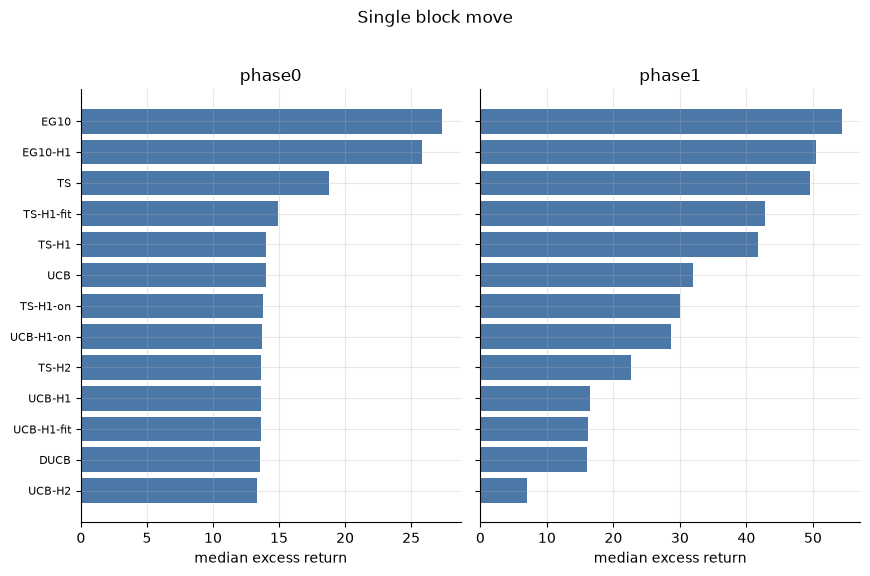
\includegraphics[width=\textwidth]{figures/policy_bar_single.png}
\caption{Single block move.
Phase 0, before the new block has majority weight, is essentially tied for every rule except epsilon-greedy.
Phase 1 median excess return is \(7.1\) for UCB at \(\eta=2\), \(16.0\) for discounted UCB, \(16.2\) for the fitted monitor at \(\eta=1\), \(32.0\) for plain UCB, and \(54.4\) for epsilon-greedy at \(10\%\).}
\end{figure}

Phase 0 is unaffected by the tax, as in the scorecard experiment.
After the move, UCB at \(\eta=2\) is the lowest median on all six pools in the single-shift path, and it is below discounted UCB.
Thompson sampling needs the larger tax: at \(\eta=2\) its phase-1 median falls from \(49.6\) to \(22.6\), still above discounted UCB.
Epsilon-greedy remains the most expensive rule in both phases.

The monitor is the practical question.
The oracle share uses every policy's realized return.
The fitted monitor does not.
It fits the reward coefficient by least squares on the transitions of the served policy, imagines every policy's return under that fit, and only then computes the residual share.
On the single move, UCB at \(\eta=1\) with the fitted monitor has median phase-1 excess \(16.2\), the same as the oracle tax at \(\eta=1\) and the same as discounted UCB.
On the second move of the double path the fitted monitor stays with the oracle: phase-2 medians are \(11.0\) for oracle UCB at \(\eta=2\), \(14.6\) for the fitted monitor at \(\eta=1\), \(16.4\) for discounted UCB, and \(42.6\) for plain UCB.
The on-policy monitor, which assigns residual \(1\) to any policy missing from a window, does not survive the second move.
Its phase-2 median is \(96\), worse than plain UCB.
A policy that was not served in the last four rounds is not a high-residual policy.
Treating missingness as risk taxes the arm one most needs to inspect.

So the deployable version of this horse-race is not ``log only what you served.''
It is ``fit the reward on what you served, imagine the other policies, and put the residual share on a discounted or undiscounted UCB index, with \(\eta\) at \(1\) or \(2\).''
Turn the tax off when the share collapses onto a single null score and the live scores are tied.
That pattern is the sign-flip failure, and it is readable from the weights alone.

\section{Operating summary}

\begin{center}
\begin{tabular}{p{0.30\textwidth}p{0.62\textwidth}}
\toprule
What the share does & Screen the score that no longer explains the batch. Release the score the batch has moved onto. \\
Relocation, gradual & UCB or discounted UCB at \(\eta=2\). Median post excess \(17.6\), against \(34.6\), \(24.6\), and \(125\) for UCB, discounted UCB, and \(\varepsilon=0.10\). \\
Relocation, drastic & Discounted UCB, tax off or very small. Median \(107.7\). The tax still beats plain UCB. \\
Dying block, nonlinear add-on & Discounted UCB at \(\eta=1\) or \(2\). Best medians \(27.1\), \(35.8\), \(2.80\), \(5.12\). \\
Sign flip & Tax off. Discount the reward. The share piles onto the zero score and the tax removes the hedge. \\
Noise growth & Thompson sampling, with a small tax. Do not discount. The best card did not change. \\
Before any shift & The tax is inert. Epsilon-greedy is not. \\
Policies & Same rule. Imagine unserved policies from a reward fit. Do not impute a residual of \(1\) for a policy you did not serve. \\
\bottomrule
\end{tabular}
\end{center}

Batch size \(200\) and pools of at least \(10{,}000\) rows are what make the comparison sharp.
The pseudo-outcome is estimated on \(1{,}200\) rows in each window, and an exploratory batch is too expensive to spend uniformly once that estimate is available.

\appendix
\section{Figures}
\graphicspath{{figures/}}

\subsection{Cumulative excess}
\newcommand{\cumfig}[2]{%
\begin{figure}[p]\centering
\includegraphics[width=\textwidth]{figures/cum_#1.png}
\caption{Cumulative excess MSE, #2. Mean across four seeds, band is the seed standard deviation. The dashed line is the first round with mixing weight at least \(1/2\).}
\end{figure}\clearpage}
\cumfig{gradual_relocate}{gradual relocation}
\cumfig{drastic_relocate}{drastic relocation}
\cumfig{gradual_flip}{gradual sign flip}
\cumfig{drastic_flip}{drastic sign flip}
\cumfig{gradual_die}{gradual dying block}
\cumfig{drastic_die}{drastic dying block}
\cumfig{gradual_nonlin}{gradual nonlinear add-on}
\cumfig{drastic_nonlin}{drastic nonlinear add-on}
\cumfig{gradual_noise}{gradual noise growth}
\cumfig{drastic_noise}{drastic noise growth}

\subsection{PO-risk shares}
\newcommand{\sharefig}[2]{%
\begin{figure}[p]\centering
\includegraphics[width=\textwidth]{figures/shares_#1.png}
\caption{PO-risk shares, #2. Mean across four seeds.}
\end{figure}\clearpage}
\sharefig{gradual_relocate}{gradual relocation}
\sharefig{drastic_relocate}{drastic relocation}
\sharefig{gradual_flip}{gradual sign flip}
\sharefig{drastic_flip}{drastic sign flip}
\sharefig{gradual_die}{gradual dying block}
\sharefig{drastic_die}{drastic dying block}
\sharefig{gradual_nonlin}{gradual nonlinear add-on}
\sharefig{drastic_nonlin}{drastic nonlinear add-on}
\sharefig{gradual_noise}{gradual noise growth}
\sharefig{drastic_noise}{drastic noise growth}

\subsection{Median rankings and the scale profile}
\newcommand{\barfig}[2]{%
\begin{figure}[p]\centering
\includegraphics[width=0.78\textwidth]{figures/bar_#1.png}
\caption{Median post-shift excess across the six pools, #2. Lower is better.}
\end{figure}\clearpage}
\barfig{gradual_relocate}{gradual relocation}
\barfig{drastic_relocate}{drastic relocation}
\barfig{gradual_flip}{gradual sign flip}
\barfig{drastic_flip}{drastic sign flip}
\barfig{gradual_die}{gradual dying block}
\barfig{drastic_die}{drastic dying block}
\barfig{gradual_nonlin}{gradual nonlinear add-on}
\barfig{drastic_nonlin}{drastic nonlinear add-on}
\barfig{gradual_noise}{gradual noise growth}
\barfig{drastic_noise}{drastic noise growth}

\begin{figure}[p]\centering
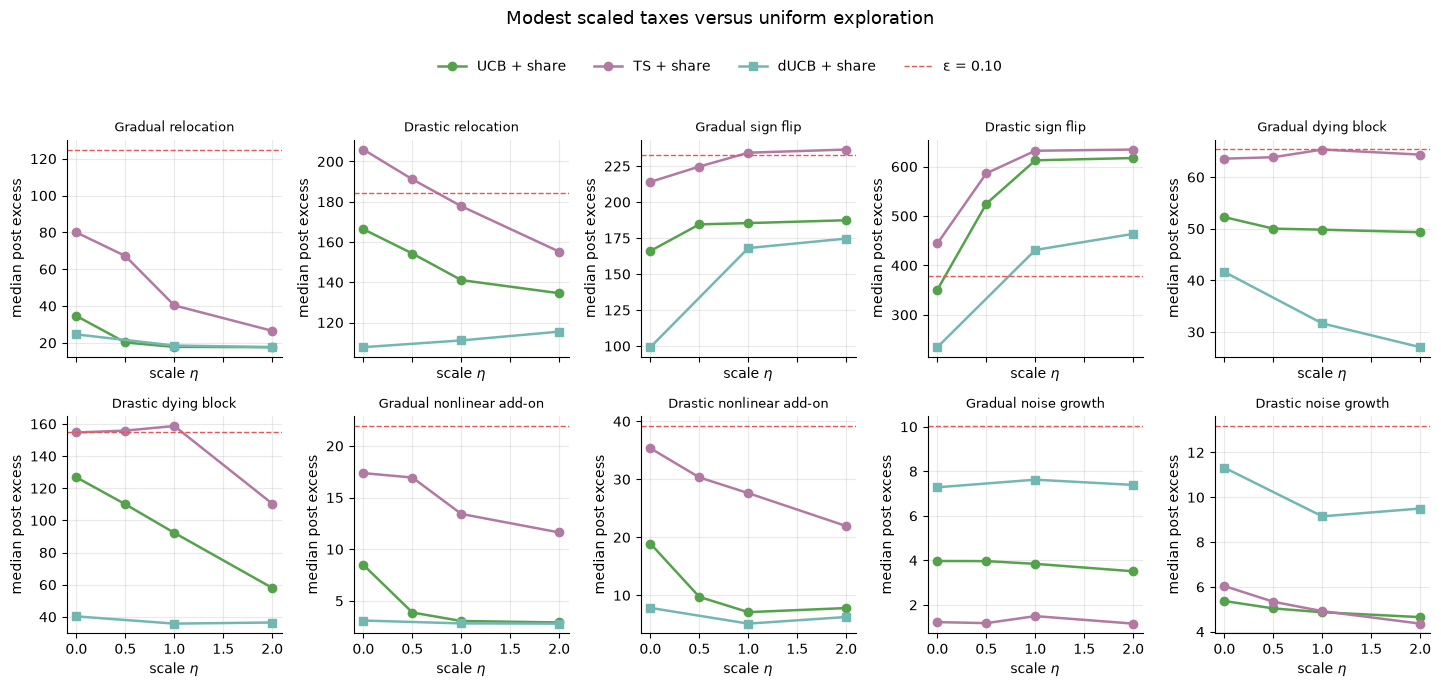
\includegraphics[width=\textwidth]{figures/eta_profile.png}
\caption{Post-shift excess against \(\eta\), median across pools.}
\end{figure}\clearpage

\subsection{Policy horse-race}
\begin{figure}[p]\centering
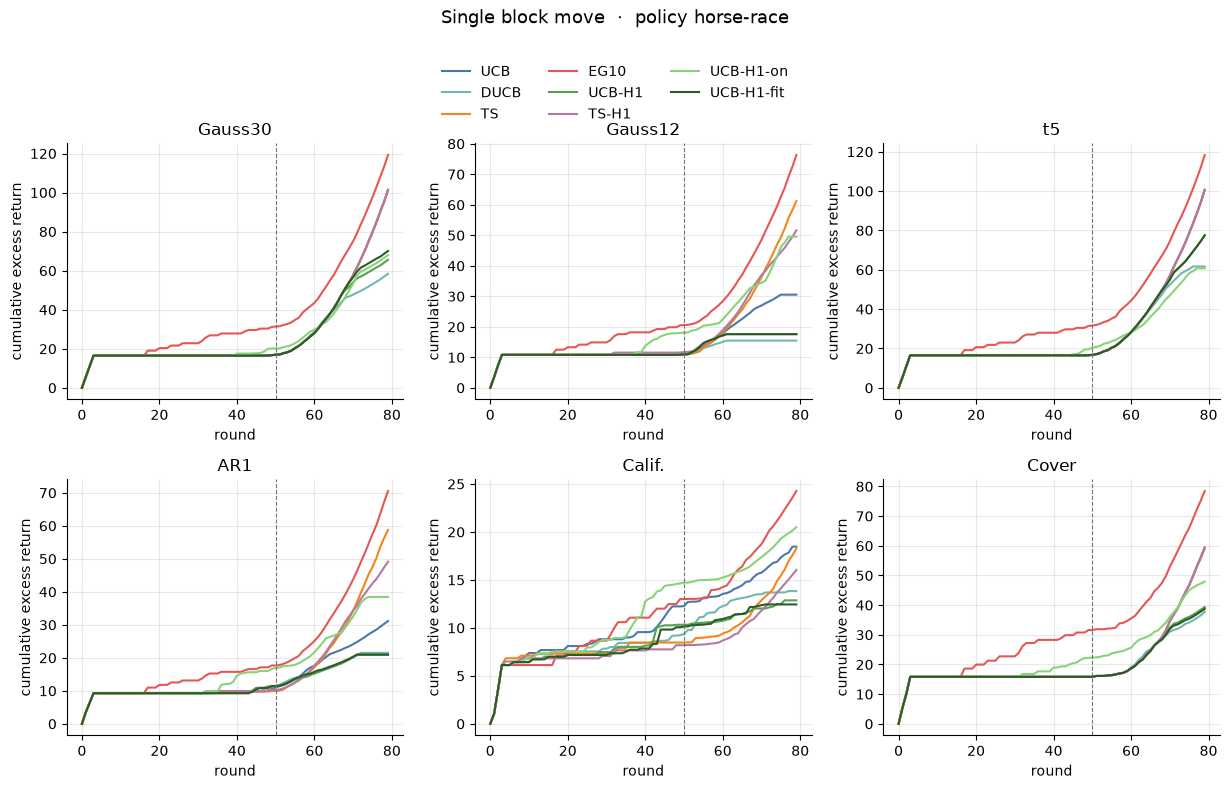
\includegraphics[width=\textwidth]{figures/policy_cum_single.png}
\caption{Cumulative excess return, single block move.}
\end{figure}\clearpage
\begin{figure}[p]\centering
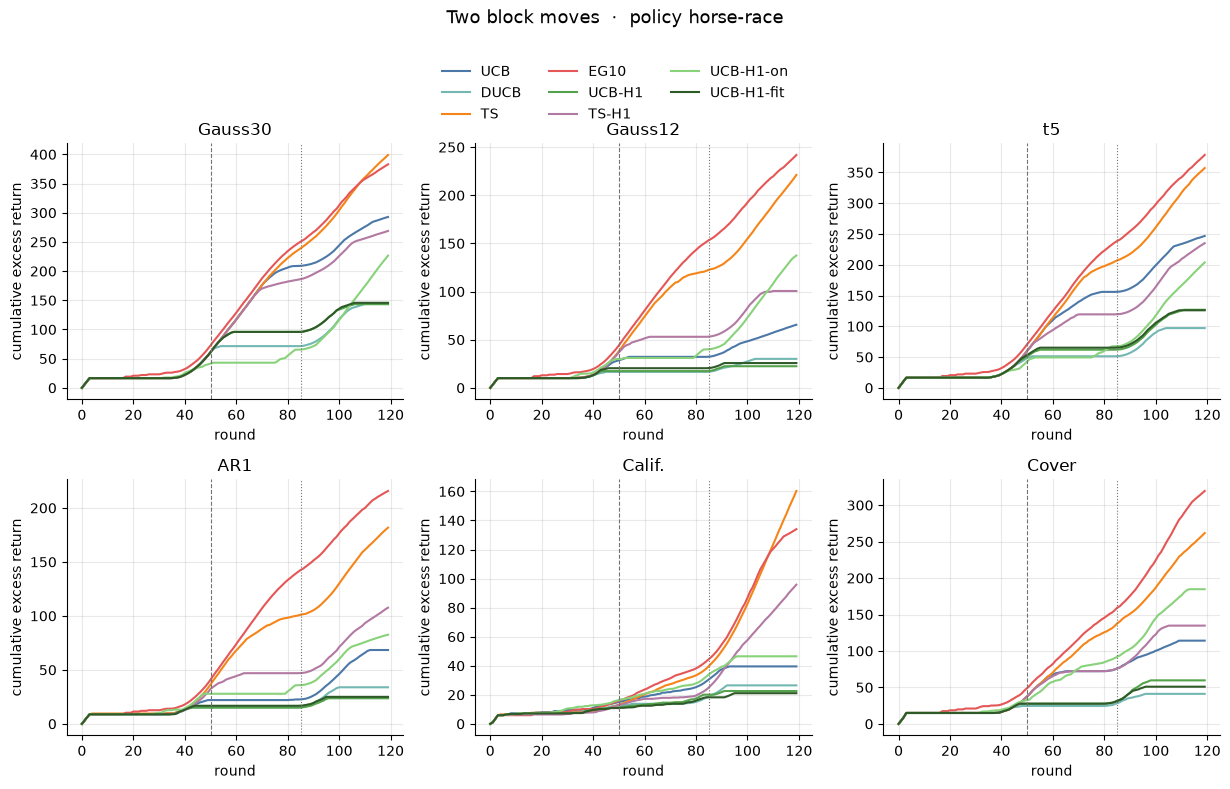
\includegraphics[width=\textwidth]{figures/policy_cum_double.png}
\caption{Cumulative excess return, two block moves. The second dashed line is the second phase.}
\end{figure}\clearpage
\begin{figure}[p]\centering
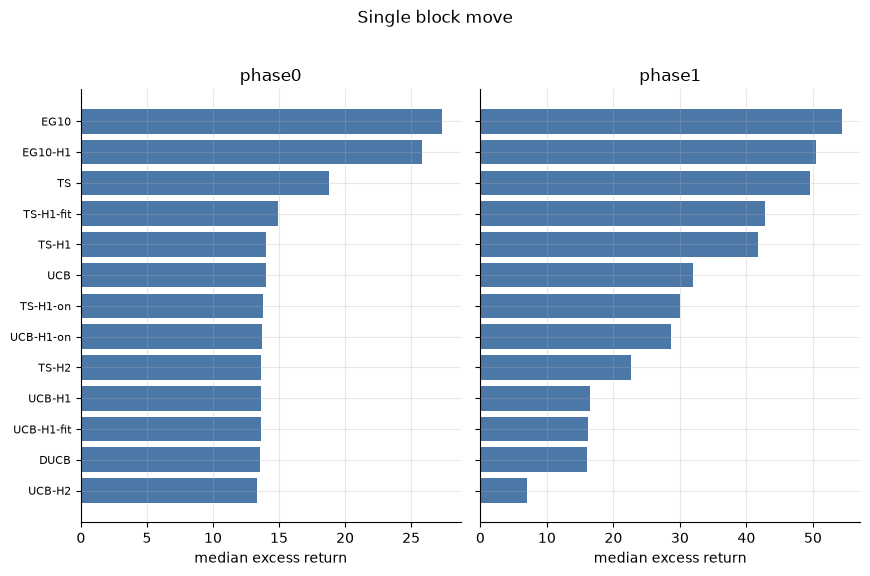
\includegraphics[width=\textwidth]{figures/policy_bar_single.png}
\caption{Median excess return, single block move.}
\end{figure}\clearpage
\begin{figure}[p]\centering
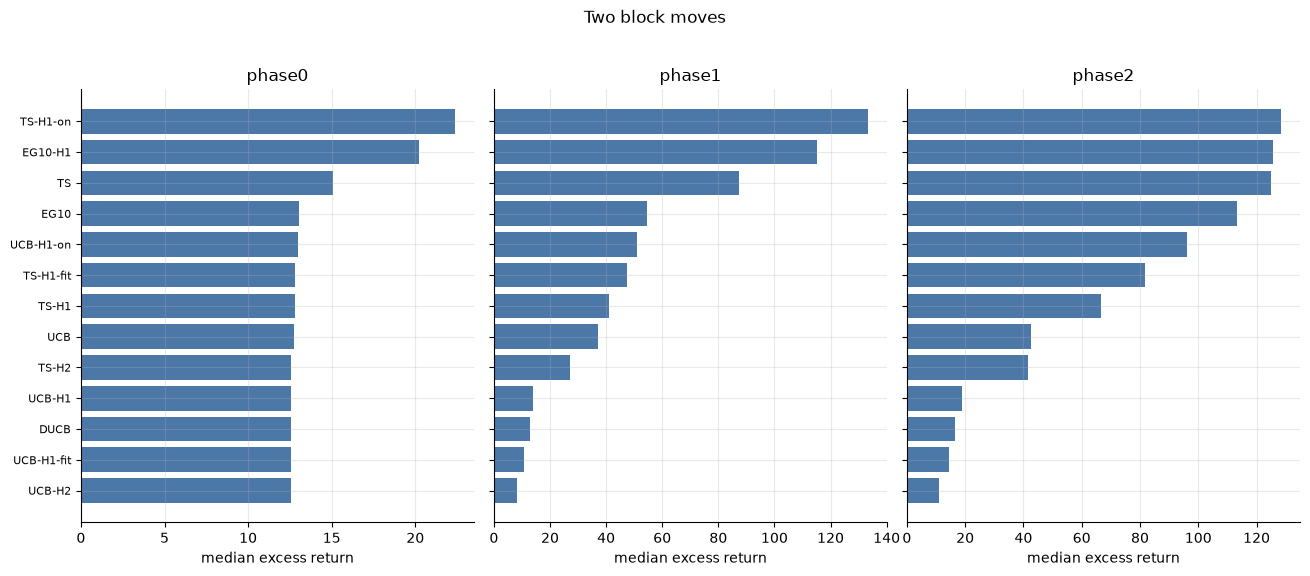
\includegraphics[width=\textwidth]{figures/policy_bar_double.png}
\caption{Median excess return, two block moves.}
\end{figure}\clearpage

\section{Tables}
\begin{table}[p]
\centering
\scriptsize
\caption{Median across covariate pools of the mean post-shift excess MSE. Each pool contributes the average over four seeds. Lower is better. The last column is the lowest median among all rules, not only the columns shown.}
\label{tab:headline}
\resizebox{\textwidth}{!}{%
\begin{tabular}{lccccccccccc}
\toprule
 & UCB & dUCB & dUCB$_{\eta=1}$ & dUCB$_{\eta=2}$ & TS & $\varepsilon$.10 & UCB$_{\eta=1}$ & UCB$_{\eta=2}$ & TS$_{\eta=2}$ & UCB$_{\lambda=5}$ & best \\
\midrule
Gradual relocation & 34.58 & 24.57 & 18.52 & 17.64 & 79.95 & 124.98 & 17.78 & 17.64 & 26.52 & 17.64 & UCB$_{\eta=2}$ \\
Drastic relocation & 166.35 & 107.75 & 111.10 & 115.47 & 205.94 & 184.12 & 141.07 & 134.55 & 155.20 & 132.39 & dUCB \\
Gradual sign flip & 166.08 & 99.25 & 168.07 & 174.65 & 214.02 & 232.78 & 185.41 & 187.38 & 236.48 & 188.67 & dUCB \\
Drastic sign flip & 350.98 & 234.64 & 431.29 & 463.92 & 444.62 & 377.94 & 612.73 & 617.39 & 634.52 & 535.59 & dUCB \\
Gradual dying block & 52.25 & 41.63 & 31.66 & 27.06 & 63.58 & 65.48 & 49.82 & 49.33 & 64.36 & 50.47 & dUCB$_{\eta=2}$ \\
Drastic dying block & 126.79 & 40.31 & 35.81 & 36.50 & 154.69 & 155.22 & 92.28 & 58.04 & 110.44 & 89.80 & dUCB$_{\eta=1}$ \\
Gradual nonlinear add-on & 8.48 & 3.10 & 2.82 & 2.80 & 17.37 & 21.93 & 3.06 & 2.91 & 11.63 & 3.15 & dUCB$_{\eta=2}$ \\
Drastic nonlinear add-on & 18.92 & 7.83 & 5.12 & 6.26 & 35.36 & 39.19 & 7.10 & 7.80 & 21.94 & 7.63 & dUCB$_{\eta=1}$ \\
Gradual noise growth & 3.97 & 7.28 & 7.62 & 7.39 & 1.23 & 10.04 & 3.84 & 3.51 & 1.16 & 3.94 & TS$_{\lambda=5}$ \\
Drastic noise growth & 5.37 & 11.32 & 9.15 & 9.50 & 6.04 & 13.18 & 4.87 & 4.65 & 4.36 & 5.16 & TS$_{\lambda=5}$ \\
\bottomrule
\end{tabular}}
\parbox{\textwidth}{\scriptsize $\eta$ multiplies the reference-window standard deviation of arm rewards. $\lambda=5$ is an absolute penalty on the share, not scaled.}
\end{table}
\clearpage

\begin{table}[p]
\centering
\scriptsize
\caption{Post-shift excess MSE: Gradual relocation. Mean over four seeds, seed standard deviation in parentheses.}
\label{tab:post:gradual_relocate}
\resizebox{\textwidth}{!}{%
\begin{tabular}{lcccccc}
\toprule
 & Gaussian $d=30$ & Gaussian $d=12$ & Student-$t_5$ & AR(1) Gaussian & California housing & Covertype \\
\midrule
UCB & 50.61 (8.51) & 22.87 (0.43) & 46.29 (4.72) & 18.22 (1.10) & 4.23 (0.63) & 73.10 (20.68) \\
dUCB & 32.71 (6.18) & 16.43 (1.31) & 34.85 (3.66) & 13.86 (0.66) & 1.65 (1.50) & 42.22 (0.64) \\
TS & 116.40 (30.74) & 69.17 (25.32) & 90.73 (25.06) & 55.57 (6.56) & 15.08 (4.61) & 125.18 (31.74) \\
$\varepsilon$.05 & 148.46 (64.87) & 61.53 (20.98) & 139.65 (66.59) & 44.88 (17.42) & 13.44 (4.51) & 164.54 (85.35) \\
$\varepsilon$.10 & 187.11 (32.16) & 79.78 (9.26) & 170.17 (33.87) & 57.42 (9.38) & 18.75 (1.63) & 216.59 (51.67) \\
$\varepsilon$.15 & 130.94 (28.90) & 49.64 (9.53) & 115.62 (21.78) & 38.70 (7.38) & 12.31 (3.73) & 135.13 (39.55) \\
UCB$_{\eta=.5}$ & 26.97 (2.90) & 15.43 (1.65) & 24.98 (1.09) & 15.01 (0.40) & 3.04 (1.27) & 37.92 (12.61) \\
UCB$_{\eta=1}$ & 25.12 (1.51) & 10.31 (0.13) & 24.98 (1.09) & 10.59 (2.12) & 3.03 (1.46) & 32.00 (1.05) \\
UCB$_{\eta=2}$ & 25.12 (1.51) & 10.31 (0.13) & 24.98 (1.09) & 8.80 (0.52) & 1.49 (0.58) & 31.17 (1.16) \\
TS$_{\eta=.5}$ & 76.00 (28.02) & 64.06 (15.24) & 70.23 (27.75) & 47.12 (7.38) & 12.91 (3.86) & 72.64 (20.20) \\
TS$_{\eta=1}$ & 54.18 (27.21) & 37.63 (18.19) & 43.02 (12.73) & 33.93 (4.65) & 9.57 (5.08) & 79.34 (49.36) \\
TS$_{\eta=2}$ & 37.17 (7.16) & 20.13 (7.30) & 32.91 (6.79) & 19.01 (7.32) & 7.76 (2.66) & 35.15 (3.04) \\
UCB$_{\lambda=5}$ & 25.12 (1.51) & 10.31 (0.13) & 24.98 (1.09) & 8.16 (0.42) & 0.23 (0.34) & 37.92 (12.61) \\
TS$_{\lambda=5}$ & 59.23 (20.17) & 18.62 (5.12) & 40.29 (9.48) & 15.45 (0.65) & 3.67 (1.41) & 75.60 (29.30) \\
$\varepsilon$.10$_{\eta=1}$ & 103.61 (15.10) & 45.62 (12.98) & 99.39 (17.96) & 33.64 (6.23) & 16.29 (5.91) & 107.87 (18.76) \\
dUCB$_{\eta=1}$ & 25.12 (1.51) & 12.06 (2.04) & 24.98 (1.09) & 11.53 (1.68) & 0.26 (0.18) & 31.17 (1.16) \\
dUCB$_{\eta=2}$ & 25.12 (1.51) & 10.31 (0.13) & 24.98 (1.09) & 8.34 (0.59) & 0.22 (0.35) & 31.17 (1.16) \\
\bottomrule
\end{tabular}}
\parbox{\textwidth}{\scriptsize Sum of per-round gaps to the best scorecard once the mixing weight reaches $1/2$.}
\end{table}
\clearpage

\begin{table}[p]
\centering
\scriptsize
\caption{Post-shift excess MSE: Drastic relocation. Mean over four seeds, seed standard deviation in parentheses.}
\label{tab:post:drastic_relocate}
\resizebox{\textwidth}{!}{%
\begin{tabular}{lcccccc}
\toprule
 & Gaussian $d=30$ & Gaussian $d=12$ & Student-$t_5$ & AR(1) Gaussian & California housing & Covertype \\
\midrule
UCB & 249.54 (8.01) & 94.33 (1.83) & 238.36 (6.20) & 75.01 (2.01) & 10.03 (2.94) & 314.64 (31.71) \\
dUCB & 161.70 (6.07) & 64.27 (1.86) & 151.22 (4.07) & 52.96 (1.23) & 6.82 (6.65) & 217.02 (28.16) \\
TS & 306.12 (7.78) & 120.61 (4.82) & 291.26 (4.01) & 95.62 (2.21) & 28.00 (1.22) & 406.47 (71.10) \\
$\varepsilon$.05 & 255.62 (5.81) & 104.08 (6.30) & 240.51 (13.15) & 82.54 (1.76) & 26.35 (3.85) & 376.86 (81.63) \\
$\varepsilon$.10 & 266.81 (10.88) & 108.43 (2.79) & 259.80 (9.02) & 85.33 (1.94) & 28.45 (5.92) & 352.51 (72.97) \\
$\varepsilon$.15 & 266.81 (13.16) & 107.10 (5.41) & 260.44 (12.15) & 85.54 (4.57) & 25.58 (2.89) & 372.09 (64.51) \\
UCB$_{\eta=.5}$ & 228.59 (5.70) & 90.53 (1.37) & 218.02 (6.87) & 72.06 (2.91) & 7.93 (1.98) & 309.14 (43.30) \\
UCB$_{\eta=1}$ & 209.62 (5.69) & 83.45 (1.63) & 198.69 (8.74) & 68.67 (2.31) & 5.57 (1.35) & 305.33 (55.07) \\
UCB$_{\eta=2}$ & 206.07 (5.29) & 72.48 (13.35) & 196.62 (9.99) & 58.78 (7.33) & 6.71 (0.88) & 286.96 (49.54) \\
TS$_{\eta=.5}$ & 280.12 (3.92) & 112.18 (2.62) & 270.12 (9.02) & 91.33 (2.74) & 25.73 (1.65) & 362.32 (42.53) \\
TS$_{\eta=1}$ & 268.78 (7.57) & 104.92 (6.31) & 250.64 (8.10) & 83.88 (4.08) & 22.89 (5.84) & 341.22 (51.00) \\
TS$_{\eta=2}$ & 224.97 (5.42) & 93.75 (4.36) & 216.64 (10.35) & 76.60 (3.77) & 20.60 (2.77) & 307.29 (55.09) \\
UCB$_{\lambda=5}$ & 208.95 (3.72) & 71.08 (16.60) & 193.70 (4.21) & 50.20 (9.99) & 7.84 (1.49) & 316.96 (65.68) \\
TS$_{\lambda=5}$ & 266.79 (5.96) & 87.36 (3.17) & 252.40 (15.42) & 63.73 (8.05) & 15.37 (6.29) & 366.06 (38.16) \\
$\varepsilon$.10$_{\eta=1}$ & 231.06 (14.03) & 94.03 (6.65) & 224.32 (19.04) & 74.73 (3.60) & 24.65 (1.99) & 342.49 (64.93) \\
dUCB$_{\eta=1}$ & 166.69 (4.55) & 63.45 (1.22) & 158.75 (5.35) & 51.09 (1.08) & 4.12 (2.41) & 216.30 (24.50) \\
dUCB$_{\eta=2}$ & 174.14 (6.29) & 66.89 (1.54) & 164.04 (9.31) & 52.56 (2.20) & 3.97 (0.34) & 232.18 (36.17) \\
\bottomrule
\end{tabular}}
\parbox{\textwidth}{\scriptsize Sum of per-round gaps to the best scorecard once the mixing weight reaches $1/2$.}
\end{table}
\clearpage

\begin{table}[p]
\centering
\scriptsize
\caption{Post-shift excess MSE: Gradual sign flip. Mean over four seeds, seed standard deviation in parentheses.}
\label{tab:post:gradual_flip}
\resizebox{\textwidth}{!}{%
\begin{tabular}{lcccccc}
\toprule
 & Gaussian $d=30$ & Gaussian $d=12$ & Student-$t_5$ & AR(1) Gaussian & California housing & Covertype \\
\midrule
UCB & 272.27 (14.77) & 63.51 (10.45) & 268.65 (20.49) & 39.79 (7.51) & 28.04 (2.94) & 349.63 (7.18) \\
dUCB & 148.69 (15.65) & 49.80 (7.16) & 155.78 (18.24) & 35.19 (2.40) & 22.40 (1.03) & 202.93 (17.80) \\
TS & 334.90 (14.05) & 97.15 (17.33) & 330.89 (10.39) & 89.30 (17.28) & 62.83 (14.16) & 423.23 (12.58) \\
$\varepsilon$.05 & 279.04 (98.84) & 122.11 (34.25) & 278.05 (102.37) & 82.59 (25.00) & 57.83 (23.55) & 353.18 (100.96) \\
$\varepsilon$.10 & 340.18 (29.58) & 138.03 (13.48) & 327.53 (23.94) & 101.38 (6.21) & 67.93 (11.21) & 430.32 (51.67) \\
$\varepsilon$.15 & 246.18 (42.88) & 107.22 (15.57) & 255.93 (31.79) & 81.21 (12.25) & 54.02 (13.24) & 329.84 (72.09) \\
UCB$_{\eta=.5}$ & 285.19 (14.86) & 94.69 (16.10) & 274.35 (13.55) & 57.24 (2.04) & 37.27 (0.78) & 370.06 (18.01) \\
UCB$_{\eta=1}$ & 287.78 (13.55) & 102.44 (10.03) & 268.38 (13.15) & 66.76 (2.50) & 44.65 (2.04) & 367.79 (20.64) \\
UCB$_{\eta=2}$ & 281.92 (19.04) & 104.33 (6.75) & 270.42 (15.66) & 67.63 (2.36) & 46.35 (1.96) & 364.21 (16.63) \\
TS$_{\eta=.5}$ & 333.78 (15.45) & 125.59 (19.74) & 323.77 (18.63) & 81.76 (9.99) & 70.13 (13.69) & 427.58 (25.12) \\
TS$_{\eta=1}$ & 337.07 (22.83) & 135.44 (11.26) & 333.18 (25.39) & 94.70 (5.86) & 67.34 (7.41) & 425.00 (24.94) \\
TS$_{\eta=2}$ & 349.34 (16.17) & 137.13 (5.55) & 335.84 (16.88) & 104.72 (4.80) & 67.54 (3.12) & 438.70 (17.82) \\
UCB$_{\lambda=5}$ & 284.25 (14.93) & 101.14 (10.13) & 276.20 (12.27) & 68.02 (1.51) & 46.54 (2.04) & 361.97 (12.23) \\
TS$_{\lambda=5}$ & 342.93 (13.39) & 134.76 (8.77) & 335.03 (10.33) & 100.24 (5.86) & 69.07 (3.23) & 424.18 (25.07) \\
$\varepsilon$.10$_{\eta=1}$ & 333.63 (33.37) & 136.04 (14.06) & 325.50 (42.42) & 100.79 (11.11) & 71.66 (7.19) & 431.92 (33.55) \\
dUCB$_{\eta=1}$ & 253.35 (10.32) & 87.75 (10.14) & 248.40 (14.26) & 55.12 (4.22) & 36.02 (1.96) & 329.53 (5.36) \\
dUCB$_{\eta=2}$ & 252.82 (9.36) & 99.89 (5.49) & 249.41 (13.03) & 66.71 (5.14) & 43.87 (3.71) & 328.25 (6.18) \\
\bottomrule
\end{tabular}}
\parbox{\textwidth}{\scriptsize Sum of per-round gaps to the best scorecard once the mixing weight reaches $1/2$.}
\end{table}
\clearpage

\begin{table}[p]
\centering
\scriptsize
\caption{Post-shift excess MSE: Drastic sign flip. Mean over four seeds, seed standard deviation in parentheses.}
\label{tab:post:drastic_flip}
\resizebox{\textwidth}{!}{%
\begin{tabular}{lcccccc}
\toprule
 & Gaussian $d=30$ & Gaussian $d=12$ & Student-$t_5$ & AR(1) Gaussian & California housing & Covertype \\
\midrule
UCB & 507.85 (14.60) & 203.27 (3.97) & 498.69 (16.25) & 147.99 (5.04) & 105.09 (3.81) & 647.66 (12.24) \\
dUCB & 331.12 (5.22) & 139.24 (2.43) & 330.04 (5.91) & 102.65 (3.62) & 75.33 (1.10) & 417.74 (11.44) \\
TS & 646.12 (15.71) & 259.37 (10.48) & 629.87 (13.88) & 191.04 (3.44) & 141.80 (4.87) & 795.40 (33.88) \\
$\varepsilon$.05 & 520.53 (5.66) & 215.25 (6.89) & 512.99 (31.75) & 161.26 (10.29) & 115.45 (4.37) & 652.30 (12.29) \\
$\varepsilon$.10 & 533.72 (1.26) & 225.03 (7.20) & 530.85 (7.06) & 162.73 (8.02) & 119.34 (5.13) & 669.45 (32.59) \\
$\varepsilon$.15 & 536.30 (17.01) & 218.68 (8.04) & 531.15 (36.12) & 166.43 (10.15) & 119.39 (4.53) & 678.69 (17.29) \\
UCB$_{\eta=.5}$ & 774.85 (28.16) & 283.24 (9.80) & 766.67 (50.32) & 195.71 (3.84) & 134.62 (2.09) & 1011.00 (52.31) \\
UCB$_{\eta=1}$ & 916.23 (11.19) & 325.52 (8.15) & 899.93 (31.79) & 228.49 (3.87) & 155.90 (3.31) & 1172.01 (21.49) \\
UCB$_{\eta=2}$ & 920.32 (13.18) & 332.46 (5.51) & 902.33 (26.14) & 239.85 (4.25) & 169.27 (4.32) & 1181.34 (23.95) \\
TS$_{\eta=.5}$ & 838.97 (35.07) & 334.04 (13.65) & 857.20 (37.11) & 235.38 (7.91) & 163.47 (5.20) & 1059.57 (14.66) \\
TS$_{\eta=1}$ & 916.51 (28.52) & 362.61 (6.56) & 901.57 (48.98) & 265.17 (3.19) & 193.77 (3.55) & 1179.96 (20.10) \\
TS$_{\eta=2}$ & 912.12 (15.54) & 367.67 (13.60) & 901.37 (16.18) & 268.20 (7.15) & 198.13 (8.84) & 1171.51 (27.73) \\
UCB$_{\lambda=5}$ & 765.75 (17.47) & 327.33 (5.89) & 743.84 (17.71) & 239.57 (4.72) & 168.99 (4.34) & 918.73 (24.42) \\
TS$_{\lambda=5}$ & 836.90 (31.88) & 364.22 (4.25) & 829.87 (36.54) & 265.65 (2.13) & 195.81 (5.37) & 1026.04 (18.49) \\
$\varepsilon$.10$_{\eta=1}$ & 911.76 (42.67) & 364.63 (20.63) & 883.02 (50.01) & 267.38 (14.50) & 192.86 (7.93) & 1151.46 (27.01) \\
dUCB$_{\eta=1}$ & 655.70 (0.90) & 228.52 (12.28) & 634.07 (32.12) & 159.66 (7.66) & 108.49 (3.46) & 788.12 (55.73) \\
dUCB$_{\eta=2}$ & 670.25 (9.12) & 270.46 (3.17) & 657.37 (16.06) & 197.05 (3.37) & 128.48 (26.53) & 860.77 (13.86) \\
\bottomrule
\end{tabular}}
\parbox{\textwidth}{\scriptsize Sum of per-round gaps to the best scorecard once the mixing weight reaches $1/2$.}
\end{table}
\clearpage

\begin{table}[p]
\centering
\scriptsize
\caption{Post-shift excess MSE: Gradual dying block. Mean over four seeds, seed standard deviation in parentheses.}
\label{tab:post:gradual_die}
\resizebox{\textwidth}{!}{%
\begin{tabular}{lcccccc}
\toprule
 & Gaussian $d=30$ & Gaussian $d=12$ & Student-$t_5$ & AR(1) Gaussian & California housing & Covertype \\
\midrule
UCB & 100.19 (2.92) & 1.95 (1.70) & 96.70 (0.57) & 7.80 (9.47) & 2.80 (1.39) & 145.04 (39.83) \\
dUCB & 82.27 (10.64) & 4.55 (2.68) & 78.70 (21.80) & 0.70 (0.96) & 0.43 (0.37) & 121.14 (70.19) \\
TS & 100.19 (2.92) & 30.45 (8.46) & 96.70 (0.57) & 30.28 (1.72) & 11.61 (0.95) & 156.07 (18.01) \\
$\varepsilon$.05 & 102.55 (5.01) & 38.98 (2.47) & 98.28 (7.28) & 30.83 (3.13) & 12.11 (2.01) & 161.70 (15.49) \\
$\varepsilon$.10 & 97.51 (8.25) & 36.84 (2.71) & 94.13 (4.53) & 28.93 (1.41) & 11.81 (1.21) & 153.59 (9.70) \\
$\varepsilon$.15 & 109.73 (8.63) & 42.03 (3.11) & 106.10 (11.36) & 32.75 (3.40) & 14.85 (3.45) & 164.01 (20.00) \\
UCB$_{\eta=.5}$ & 100.19 (2.92) & 3.16 (3.25) & 96.70 (0.57) & 3.34 (2.94) & 2.25 (0.71) & 141.53 (46.83) \\
UCB$_{\eta=1}$ & 100.19 (2.92) & 2.84 (1.75) & 96.70 (0.57) & 2.94 (4.03) & 0.72 (0.35) & 139.07 (51.73) \\
UCB$_{\eta=2}$ & 100.19 (2.92) & 3.60 (1.95) & 95.06 (3.65) & 2.53 (3.37) & 0.73 (0.61) & 132.97 (63.90) \\
TS$_{\eta=.5}$ & 100.19 (2.92) & 31.01 (8.60) & 96.70 (0.57) & 28.34 (3.95) & 11.61 (0.95) & 159.13 (12.12) \\
TS$_{\eta=1}$ & 100.19 (2.92) & 33.98 (8.30) & 96.70 (0.57) & 27.64 (4.83) & 11.79 (0.84) & 150.60 (28.79) \\
TS$_{\eta=2}$ & 100.19 (2.92) & 32.03 (10.55) & 96.70 (0.57) & 25.96 (4.27) & 10.67 (2.10) & 148.50 (32.95) \\
UCB$_{\lambda=5}$ & 100.19 (2.92) & 4.24 (2.28) & 96.70 (0.57) & 2.59 (3.33) & 0.99 (0.84) & 141.53 (46.83) \\
TS$_{\lambda=5}$ & 100.19 (2.92) & 30.20 (11.02) & 96.70 (0.57) & 26.97 (6.52) & 11.35 (1.08) & 159.13 (12.12) \\
$\varepsilon$.10$_{\eta=1}$ & 105.89 (2.11) & 40.61 (1.68) & 102.14 (4.15) & 31.57 (1.69) & 13.43 (2.61) & 161.84 (13.73) \\
dUCB$_{\eta=1}$ & 60.07 (9.11) & 4.18 (1.65) & 59.14 (15.82) & 0.40 (0.20) & 0.25 (0.15) & 109.06 (67.14) \\
dUCB$_{\eta=2}$ & 53.42 (1.17) & 4.99 (1.85) & 49.14 (10.26) & 1.39 (1.04) & 0.35 (0.15) & 100.40 (71.89) \\
\bottomrule
\end{tabular}}
\parbox{\textwidth}{\scriptsize Sum of per-round gaps to the best scorecard once the mixing weight reaches $1/2$.}
\end{table}
\clearpage

\begin{table}[p]
\centering
\scriptsize
\caption{Post-shift excess MSE: Drastic dying block. Mean over four seeds, seed standard deviation in parentheses.}
\label{tab:post:drastic_die}
\resizebox{\textwidth}{!}{%
\begin{tabular}{lcccccc}
\toprule
 & Gaussian $d=30$ & Gaussian $d=12$ & Student-$t_5$ & AR(1) Gaussian & California housing & Covertype \\
\midrule
UCB & 260.38 (8.77) & 14.39 (5.79) & 230.55 (37.96) & 23.02 (5.00) & 7.85 (3.66) & 350.17 (166.91) \\
dUCB & 73.71 (10.02) & 10.61 (3.27) & 70.02 (27.50) & 8.19 (6.73) & 1.54 (1.13) & 190.27 (164.61) \\
TS & 230.11 (61.06) & 72.54 (32.53) & 253.31 (5.46) & 79.27 (4.07) & 31.82 (2.81) & 325.72 (132.51) \\
$\varepsilon$.05 & 250.02 (22.39) & 98.82 (3.87) & 252.01 (9.17) & 77.43 (3.78) & 31.74 (3.52) & 409.33 (41.98) \\
$\varepsilon$.10 & 221.90 (38.75) & 88.54 (15.41) & 223.25 (38.27) & 68.79 (11.88) & 28.80 (6.57) & 327.10 (49.96) \\
$\varepsilon$.15 & 254.41 (23.74) & 99.34 (6.26) & 246.06 (28.21) & 75.23 (8.46) & 32.88 (4.77) & 368.30 (82.72) \\
UCB$_{\eta=.5}$ & 216.93 (26.52) & 19.92 (2.39) & 200.14 (51.67) & 18.62 (3.15) & 4.67 (1.59) & 308.90 (170.65) \\
UCB$_{\eta=1}$ & 174.07 (34.70) & 20.70 (2.07) & 163.86 (54.75) & 9.87 (7.17) & 4.04 (2.52) & 280.93 (179.90) \\
UCB$_{\eta=2}$ & 103.44 (31.15) & 20.02 (1.02) & 96.06 (32.73) & 12.30 (3.52) & 3.58 (1.99) & 265.37 (175.46) \\
TS$_{\eta=.5}$ & 262.48 (6.15) & 57.33 (16.03) & 241.52 (24.35) & 70.18 (18.17) & 31.82 (2.81) & 354.97 (148.53) \\
TS$_{\eta=1}$ & 256.88 (8.36) & 49.38 (17.32) & 248.44 (10.71) & 68.98 (19.34) & 26.54 (10.54) & 303.59 (155.57) \\
TS$_{\eta=2}$ & 202.80 (56.22) & 35.10 (9.51) & 180.97 (75.18) & 39.90 (29.18) & 19.66 (6.69) & 274.86 (166.23) \\
UCB$_{\lambda=5}$ & 170.52 (32.22) & 20.02 (1.02) & 159.58 (56.10) & 15.21 (0.42) & 6.79 (0.84) & 308.90 (170.65) \\
TS$_{\lambda=5}$ & 240.04 (45.91) & 34.14 (10.15) & 226.69 (41.78) & 27.78 (12.95) & 10.08 (4.38) & 312.93 (168.78) \\
$\varepsilon$.10$_{\eta=1}$ & 232.65 (55.69) & 93.37 (11.62) & 225.34 (42.81) & 69.04 (16.13) & 31.97 (5.18) & 313.40 (70.18) \\
dUCB$_{\eta=1}$ & 54.33 (1.91) & 17.60 (3.70) & 54.03 (4.91) & 5.24 (2.60) & 1.90 (0.98) & 157.25 (112.74) \\
dUCB$_{\eta=2}$ & 52.47 (2.00) & 20.70 (2.07) & 52.31 (2.16) & 9.70 (3.99) & 2.46 (0.60) & 132.65 (106.33) \\
\bottomrule
\end{tabular}}
\parbox{\textwidth}{\scriptsize Sum of per-round gaps to the best scorecard once the mixing weight reaches $1/2$.}
\end{table}
\clearpage

\begin{table}[p]
\centering
\scriptsize
\caption{Post-shift excess MSE: Gradual nonlinear add-on. Mean over four seeds, seed standard deviation in parentheses.}
\label{tab:post:gradual_nonlin}
\resizebox{\textwidth}{!}{%
\begin{tabular}{lcccccc}
\toprule
 & Gaussian $d=30$ & Gaussian $d=12$ & Student-$t_5$ & AR(1) Gaussian & California housing & Covertype \\
\midrule
UCB & 2.34 (0.28) & 2.27 (0.48) & 13.14 (11.69) & 3.82 (1.18) & 1745.25 (2817.19) & 228.43 (35.78) \\
dUCB & 0.28 (0.13) & 0.16 (0.15) & 5.92 (9.64) & 0.10 (0.03) & 1695.80 (2855.67) & 110.64 (110.75) \\
TS & 10.41 (0.69) & 11.18 (0.70) & 23.55 (2.92) & 10.82 (1.21) & 290.75 (200.52) & 226.84 (35.44) \\
$\varepsilon$.05 & 16.37 (8.45) & 12.73 (3.45) & 27.71 (13.57) & 12.27 (3.83) & 1669.34 (2873.04) & 234.10 (48.58) \\
$\varepsilon$.10 & 16.08 (12.24) & 12.23 (4.79) & 27.78 (12.81) & 11.71 (3.45) & 1719.57 (2825.33) & 225.68 (38.72) \\
$\varepsilon$.15 & 38.94 (16.69) & 20.82 (5.76) & 51.30 (15.82) & 18.07 (5.37) & 225.21 (158.71) & 258.15 (50.00) \\
UCB$_{\eta=.5}$ & 0.92 (0.27) & 1.05 (0.11) & 6.21 (9.48) & 1.54 (0.95) & 198.69 (191.21) & 208.56 (19.91) \\
UCB$_{\eta=1}$ & 0.47 (0.09) & 0.53 (0.14) & 5.58 (9.88) & 0.41 (0.17) & 200.73 (194.17) & 161.24 (70.04) \\
UCB$_{\eta=2}$ & 0.43 (0.18) & 0.37 (0.10) & 5.40 (10.00) & 0.32 (0.08) & 180.34 (209.10) & 94.76 (83.06) \\
TS$_{\eta=.5}$ & 10.41 (0.69) & 10.59 (0.64) & 23.13 (3.86) & 10.75 (1.22) & 192.72 (191.70) & 226.84 (35.44) \\
TS$_{\eta=1}$ & 10.41 (0.69) & 10.59 (0.64) & 16.24 (3.55) & 10.37 (0.55) & 182.45 (205.13) & 211.62 (18.82) \\
TS$_{\eta=2}$ & 9.52 (1.92) & 9.77 (2.22) & 12.50 (7.64) & 10.75 (1.22) & 170.26 (213.06) & 140.07 (97.89) \\
UCB$_{\lambda=5}$ & 0.64 (0.28) & 0.19 (0.12) & 5.67 (9.81) & 0.29 (0.01) & 1732.79 (2836.28) & 208.56 (19.91) \\
TS$_{\lambda=5}$ & 10.41 (0.69) & 10.59 (0.64) & 17.23 (3.21) & 10.79 (0.93) & 266.52 (236.04) & 226.84 (35.44) \\
$\varepsilon$.10$_{\eta=1}$ & 28.93 (17.23) & 16.77 (4.71) & 40.74 (14.47) & 16.28 (5.58) & 192.49 (191.80) & 239.38 (28.46) \\
dUCB$_{\eta=1}$ & 0.27 (0.06) & 0.13 (0.08) & 5.38 (10.01) & 0.19 (0.10) & 183.81 (205.39) & 88.84 (102.20) \\
dUCB$_{\eta=2}$ & 0.30 (0.11) & 0.13 (0.07) & 5.30 (10.05) & 0.25 (0.09) & 176.81 (213.17) & 56.02 (48.53) \\
\bottomrule
\end{tabular}}
\parbox{\textwidth}{\scriptsize Sum of per-round gaps to the best scorecard once the mixing weight reaches $1/2$.}
\end{table}
\clearpage

\begin{table}[p]
\centering
\scriptsize
\caption{Post-shift excess MSE: Drastic nonlinear add-on. Mean over four seeds, seed standard deviation in parentheses.}
\label{tab:post:drastic_nonlin}
\resizebox{\textwidth}{!}{%
\begin{tabular}{lcccccc}
\toprule
 & Gaussian $d=30$ & Gaussian $d=12$ & Student-$t_5$ & AR(1) Gaussian & California housing & Covertype \\
\midrule
UCB & 4.69 (0.52) & 5.35 (1.85) & 31.74 (25.27) & 6.09 (1.31) & 6881.65 (8936.77) & 359.45 (170.25) \\
dUCB & 1.75 (0.26) & 1.70 (0.81) & 13.91 (25.84) & 1.34 (0.16) & 5289.18 (9742.23) & 128.53 (66.51) \\
TS & 24.64 (5.43) & 28.26 (1.07) & 42.46 (10.26) & 24.82 (4.64) & 5576.16 (9369.74) & 442.39 (128.64) \\
$\varepsilon$.05 & 33.15 (8.38) & 29.37 (3.17) & 54.93 (20.19) & 26.92 (5.45) & 5102.50 (9676.15) & 535.73 (93.55) \\
$\varepsilon$.10 & 29.50 (14.98) & 26.34 (7.39) & 48.88 (10.97) & 23.82 (6.56) & 6709.47 (9080.82) & 439.94 (78.74) \\
$\varepsilon$.15 & 54.11 (19.54) & 36.76 (7.14) & 76.64 (24.35) & 32.85 (6.54) & 5300.45 (9558.91) & 484.08 (161.92) \\
UCB$_{\eta=.5}$ & 1.53 (0.19) & 2.04 (0.33) & 16.51 (24.41) & 2.93 (1.26) & 4995.11 (9759.41) & 286.82 (217.37) \\
UCB$_{\eta=1}$ & 2.00 (1.07) & 2.33 (0.69) & 11.27 (17.35) & 2.92 (1.51) & 4995.05 (9761.10) & 250.04 (243.91) \\
UCB$_{\eta=2}$ & 3.38 (0.92) & 3.39 (0.78) & 12.21 (5.53) & 2.99 (0.44) & 4993.54 (9757.37) & 215.55 (175.16) \\
TS$_{\eta=.5}$ & 26.99 (0.47) & 28.29 (2.45) & 32.37 (16.01) & 27.96 (0.79) & 4995.24 (9750.92) & 360.84 (189.26) \\
TS$_{\eta=1}$ & 23.99 (6.72) & 27.65 (1.30) & 27.58 (16.99) & 23.46 (6.79) & 4993.10 (9755.40) & 293.36 (222.07) \\
TS$_{\eta=2}$ & 13.51 (8.27) & 14.15 (3.21) & 24.50 (19.20) & 19.38 (5.17) & 4991.48 (9754.37) & 262.87 (237.63) \\
UCB$_{\lambda=5}$ & 2.02 (0.85) & 4.74 (0.30) & 10.52 (16.79) & 3.48 (0.38) & 5269.94 (9578.09) & 281.62 (221.39) \\
TS$_{\lambda=5}$ & 24.85 (5.01) & 11.87 (5.06) & 25.45 (18.86) & 11.40 (1.89) & 5333.57 (9524.38) & 303.08 (221.35) \\
$\varepsilon$.10$_{\eta=1}$ & 51.90 (17.10) & 33.34 (6.62) & 63.37 (23.17) & 32.36 (6.48) & 5053.59 (9716.62) & 503.13 (143.42) \\
dUCB$_{\eta=1}$ & 1.50 (0.31) & 1.91 (0.70) & 8.33 (12.25) & 1.56 (1.13) & 4992.45 (9757.10) & 123.65 (60.02) \\
dUCB$_{\eta=2}$ & 3.57 (0.81) & 3.38 (1.34) & 8.95 (7.15) & 2.21 (0.32) & 4994.98 (9756.30) & 131.83 (34.99) \\
\bottomrule
\end{tabular}}
\parbox{\textwidth}{\scriptsize Sum of per-round gaps to the best scorecard once the mixing weight reaches $1/2$.}
\end{table}
\clearpage

\begin{table}[p]
\centering
\scriptsize
\caption{Post-shift excess MSE: Gradual noise growth. Mean over four seeds, seed standard deviation in parentheses.}
\label{tab:post:gradual_noise}
\resizebox{\textwidth}{!}{%
\begin{tabular}{lcccccc}
\toprule
 & Gaussian $d=30$ & Gaussian $d=12$ & Student-$t_5$ & AR(1) Gaussian & California housing & Covertype \\
\midrule
UCB & 3.00 (0.54) & 5.02 (1.26) & 3.09 (1.35) & 4.85 (0.78) & 7.81 (0.63) & 2.86 (1.18) \\
dUCB & 6.22 (0.92) & 8.34 (0.74) & 5.44 (0.79) & 11.12 (3.45) & 11.76 (0.55) & 6.20 (0.63) \\
TS & 0.36 (0.73) & 3.41 (1.77) & 0.35 (0.71) & 1.90 (0.27) & 3.69 (1.85) & 0.55 (1.10) \\
$\varepsilon$.05 & 7.86 (5.96) & 3.04 (2.28) & 6.61 (6.34) & 2.90 (2.44) & 2.26 (1.15) & 10.04 (8.62) \\
$\varepsilon$.10 & 14.46 (12.59) & 6.87 (3.92) & 13.20 (11.69) & 4.96 (3.91) & 3.47 (1.13) & 18.51 (15.75) \\
$\varepsilon$.15 & 31.47 (12.47) & 12.53 (4.46) & 29.34 (10.63) & 9.69 (3.86) & 4.90 (0.89) & 39.38 (13.40) \\
UCB$_{\eta=.5}$ & 3.15 (0.53) & 5.56 (0.76) & 2.96 (1.04) & 4.78 (0.28) & 7.33 (0.89) & 2.68 (1.34) \\
UCB$_{\eta=1}$ & 3.18 (0.22) & 4.31 (1.92) & 2.48 (1.09) & 4.86 (0.58) & 7.33 (0.72) & 3.38 (1.44) \\
UCB$_{\eta=2}$ & 2.79 (0.09) & 4.95 (1.66) & 1.81 (0.54) & 4.09 (1.46) & 7.84 (1.50) & 2.93 (1.44) \\
TS$_{\eta=.5}$ & 0.00 (0.00) & 2.36 (0.67) & 0.00 (0.00) & 2.49 (1.14) & 2.99 (1.07) & 0.00 (0.00) \\
TS$_{\eta=1}$ & 0.00 (0.00) & 3.63 (2.05) & 0.00 (0.00) & 3.30 (1.84) & 2.99 (1.73) & 0.00 (0.00) \\
TS$_{\eta=2}$ & 0.00 (0.00) & 2.15 (0.49) & 0.25 (0.50) & 2.07 (0.84) & 3.05 (1.83) & 0.00 (0.00) \\
UCB$_{\lambda=5}$ & 3.18 (0.22) & 5.06 (1.66) & 2.48 (1.09) & 4.60 (0.23) & 6.42 (0.31) & 3.28 (1.57) \\
TS$_{\lambda=5}$ & 0.00 (0.00) & 2.06 (0.52) & 0.36 (0.72) & 1.39 (0.54) & 1.90 (0.71) & 0.42 (0.84) \\
$\varepsilon$.10$_{\eta=1}$ & 23.16 (19.45) & 8.40 (6.70) & 19.95 (17.99) & 8.73 (7.14) & 3.53 (2.38) & 38.65 (39.72) \\
dUCB$_{\eta=1}$ & 5.92 (0.60) & 9.03 (1.14) & 6.22 (0.90) & 9.23 (3.35) & 11.33 (0.49) & 5.73 (0.94) \\
dUCB$_{\eta=2}$ & 5.62 (1.24) & 8.49 (1.13) & 6.29 (0.47) & 8.72 (2.66) & 10.73 (1.04) & 4.88 (0.91) \\
\bottomrule
\end{tabular}}
\parbox{\textwidth}{\scriptsize Sum of per-round gaps to the best scorecard once the mixing weight reaches $1/2$.}
\end{table}
\clearpage

\begin{table}[p]
\centering
\scriptsize
\caption{Post-shift excess MSE: Drastic noise growth. Mean over four seeds, seed standard deviation in parentheses.}
\label{tab:post:drastic_noise}
\resizebox{\textwidth}{!}{%
\begin{tabular}{lcccccc}
\toprule
 & Gaussian $d=30$ & Gaussian $d=12$ & Student-$t_5$ & AR(1) Gaussian & California housing & Covertype \\
\midrule
UCB & 3.48 (0.54) & 7.09 (1.18) & 3.63 (1.00) & 10.31 (3.18) & 10.57 (0.90) & 3.66 (0.23) \\
dUCB & 7.94 (2.27) & 15.65 (1.69) & 6.72 (3.06) & 14.69 (2.71) & 15.06 (0.46) & 6.12 (0.66) \\
TS & 3.97 (0.77) & 7.72 (2.49) & 3.87 (1.58) & 7.02 (1.79) & 10.55 (1.35) & 5.06 (0.95) \\
$\varepsilon$.05 & 10.28 (2.82) & 3.90 (1.78) & 8.85 (4.13) & 3.45 (2.21) & 4.11 (0.83) & 12.78 (5.51) \\
$\varepsilon$.10 & 19.05 (10.53) & 8.38 (3.30) & 17.97 (9.67) & 6.14 (3.05) & 5.43 (0.64) & 24.78 (12.44) \\
$\varepsilon$.15 & 35.66 (16.35) & 14.40 (6.34) & 33.39 (14.27) & 11.59 (4.79) & 7.71 (2.18) & 44.01 (18.56) \\
UCB$_{\eta=.5}$ & 3.45 (0.49) & 5.94 (0.47) & 3.54 (0.87) & 9.15 (4.33) & 10.01 (0.33) & 4.15 (0.65) \\
UCB$_{\eta=1}$ & 3.38 (0.55) & 6.33 (0.68) & 3.30 (0.49) & 8.23 (2.75) & 9.62 (0.37) & 3.41 (0.83) \\
UCB$_{\eta=2}$ & 3.13 (0.16) & 6.17 (0.75) & 3.13 (0.66) & 7.20 (1.80) & 8.83 (1.11) & 2.64 (0.57) \\
TS$_{\eta=.5}$ & 3.27 (1.09) & 6.62 (2.22) & 3.34 (0.81) & 7.21 (3.15) & 9.56 (1.66) & 4.05 (0.46) \\
TS$_{\eta=1}$ & 4.45 (0.84) & 7.51 (3.33) & 4.53 (1.12) & 5.31 (1.59) & 7.94 (1.25) & 4.26 (0.81) \\
TS$_{\eta=2}$ & 3.87 (0.41) & 4.62 (1.36) & 4.10 (1.18) & 4.68 (2.10) & 8.22 (1.05) & 3.89 (0.76) \\
UCB$_{\lambda=5}$ & 3.19 (0.20) & 6.18 (0.70) & 3.30 (0.49) & 6.79 (2.45) & 8.27 (0.81) & 4.15 (0.65) \\
TS$_{\lambda=5}$ & 3.78 (1.30) & 3.65 (1.54) & 3.79 (1.00) & 4.62 (2.05) & 8.50 (1.70) & 5.20 (1.12) \\
$\varepsilon$.10$_{\eta=1}$ & 35.39 (19.28) & 12.98 (6.61) & 31.75 (17.23) & 12.43 (7.39) & 6.17 (2.43) & 53.75 (42.59) \\
dUCB$_{\eta=1}$ & 6.70 (0.32) & 11.60 (3.76) & 5.84 (0.51) & 13.35 (1.86) & 13.56 (1.11) & 5.81 (0.72) \\
dUCB$_{\eta=2}$ & 6.89 (0.56) & 12.10 (3.32) & 5.90 (0.73) & 12.25 (2.17) & 13.27 (0.65) & 5.85 (0.66) \\
\bottomrule
\end{tabular}}
\parbox{\textwidth}{\scriptsize Sum of per-round gaps to the best scorecard once the mixing weight reaches $1/2$.}
\end{table}
\clearpage

\begin{table}[p]
\centering
\scriptsize
\caption{Ramp excess MSE: Gradual relocation. Rounds with mixing weight in $(0,1/2)$.}
\label{tab:ramp:gradual_relocate}
\resizebox{\textwidth}{!}{%
\begin{tabular}{lcccccc}
\toprule
 & Gaussian $d=30$ & Gaussian $d=12$ & Student-$t_5$ & AR(1) Gaussian & California housing & Covertype \\
\midrule
UCB & 24.03 (0.74) & 2.16 (0.51) & 16.27 (10.05) & 3.32 (0.57) & 3.44 (0.17) & 24.58 (7.75) \\
dUCB & 16.55 (3.94) & 0.90 (0.78) & 10.18 (6.00) & 1.29 (0.71) & 1.11 (0.61) & 15.72 (9.72) \\
TS & 24.03 (0.74) & 9.43 (0.32) & 23.48 (0.85) & 7.97 (0.95) & 2.25 (0.11) & 28.42 (0.36) \\
$\varepsilon$.05 & 30.26 (5.36) & 12.23 (2.18) & 29.63 (4.44) & 9.23 (1.72) & 2.94 (0.47) & 36.53 (6.31) \\
$\varepsilon$.10 & 34.07 (6.10) & 13.56 (2.34) & 34.07 (7.79) & 10.57 (2.18) & 3.67 (1.04) & 41.62 (8.92) \\
$\varepsilon$.15 & 41.75 (10.06) & 16.84 (5.26) & 39.31 (9.36) & 13.15 (3.19) & 4.20 (1.44) & 50.18 (13.80) \\
UCB$_{\eta=.5}$ & 20.26 (3.36) & 0.97 (0.36) & 13.83 (7.69) & 2.02 (0.55) & 2.74 (0.69) & 22.41 (4.67) \\
UCB$_{\eta=1}$ & 17.92 (0.95) & 0.72 (0.23) & 13.62 (7.21) & 0.94 (0.37) & 2.29 (0.43) & 23.21 (3.85) \\
UCB$_{\eta=2}$ & 17.92 (0.95) & 0.97 (0.13) & 13.62 (7.21) & 0.76 (0.29) & 1.47 (0.43) & 21.19 (0.37) \\
TS$_{\eta=.5}$ & 24.03 (0.74) & 9.43 (0.32) & 23.48 (0.85) & 7.41 (0.26) & 2.71 (0.90) & 25.15 (6.61) \\
TS$_{\eta=1}$ & 21.82 (4.71) & 8.73 (1.29) & 21.14 (4.67) & 7.34 (0.38) & 2.83 (0.70) & 28.42 (0.36) \\
TS$_{\eta=2}$ & 24.03 (0.74) & 8.58 (1.97) & 21.29 (3.78) & 7.47 (0.54) & 2.62 (0.76) & 25.13 (6.73) \\
UCB$_{\lambda=5}$ & 17.92 (0.95) & 1.04 (0.08) & 13.04 (6.98) & 0.79 (0.05) & 0.34 (0.14) & 22.41 (4.67) \\
TS$_{\lambda=5}$ & 24.03 (0.74) & 9.02 (0.66) & 22.77 (2.20) & 7.34 (0.38) & 2.27 (0.34) & 27.73 (1.60) \\
$\varepsilon$.10$_{\eta=1}$ & 33.45 (3.05) & 13.32 (1.71) & 33.44 (1.75) & 10.28 (1.33) & 4.04 (0.54) & 40.10 (4.22) \\
dUCB$_{\eta=1}$ & 15.84 (2.77) & 0.90 (0.33) & 10.18 (6.00) & 0.46 (0.34) & 1.59 (0.70) & 14.37 (5.22) \\
dUCB$_{\eta=2}$ & 16.58 (1.73) & 0.96 (0.25) & 10.18 (6.00) & 0.79 (0.05) & 1.15 (0.74) & 12.96 (5.56) \\
\bottomrule
\end{tabular}}
\parbox{\textwidth}{\scriptsize The ramp is where a historical mean is already stale and the fresh arm is not yet dominant.}
\end{table}
\clearpage

\begin{table}[p]
\centering
\scriptsize
\caption{Ramp excess MSE: Gradual sign flip. Rounds with mixing weight in $(0,1/2)$.}
\label{tab:ramp:gradual_flip}
\resizebox{\textwidth}{!}{%
\begin{tabular}{lcccccc}
\toprule
 & Gaussian $d=30$ & Gaussian $d=12$ & Student-$t_5$ & AR(1) Gaussian & California housing & Covertype \\
\midrule
UCB & 16.76 (2.60) & 6.37 (1.98) & 16.71 (1.71) & 5.42 (0.76) & 3.99 (1.62) & 20.53 (2.63) \\
dUCB & 13.02 (3.19) & 4.49 (0.45) & 13.17 (1.77) & 4.29 (1.03) & 4.10 (0.78) & 14.04 (2.42) \\
TS & 55.63 (5.75) & 23.63 (0.71) & 58.30 (2.37) & 16.24 (1.40) & 12.97 (0.52) & 63.73 (10.80) \\
$\varepsilon$.05 & 70.56 (9.51) & 29.39 (4.29) & 72.75 (11.38) & 20.98 (2.99) & 16.15 (2.51) & 90.73 (12.42) \\
$\varepsilon$.10 & 68.13 (9.79) & 27.68 (4.77) & 71.93 (10.24) & 19.96 (2.67) & 14.68 (2.18) & 85.44 (14.75) \\
$\varepsilon$.15 & 85.02 (12.21) & 35.00 (6.03) & 85.88 (14.38) & 25.81 (4.03) & 19.62 (2.90) & 109.85 (19.10) \\
UCB$_{\eta=.5}$ & 15.97 (3.76) & 7.45 (0.95) & 15.84 (2.53) & 4.89 (0.98) & 3.82 (0.48) & 23.49 (1.12) \\
UCB$_{\eta=1}$ & 16.41 (3.82) & 6.70 (0.69) & 16.34 (4.00) & 5.31 (0.55) & 3.51 (0.56) & 22.45 (0.70) \\
UCB$_{\eta=2}$ & 14.27 (1.97) & 6.37 (0.48) & 16.25 (4.09) & 5.09 (0.41) & 4.16 (0.71) & 23.21 (3.36) \\
TS$_{\eta=.5}$ & 46.26 (6.33) & 21.10 (3.43) & 45.70 (8.40) & 14.19 (2.03) & 12.02 (1.81) & 63.19 (8.06) \\
TS$_{\eta=1}$ & 51.43 (10.74) & 21.14 (3.64) & 53.83 (9.00) & 16.17 (1.64) & 11.87 (1.61) & 60.44 (7.27) \\
TS$_{\eta=2}$ & 56.45 (3.55) & 21.77 (1.78) & 54.64 (6.20) & 16.84 (0.60) & 10.98 (1.13) & 64.67 (8.42) \\
UCB$_{\lambda=5}$ & 16.94 (2.97) & 7.32 (0.59) & 15.84 (2.53) & 5.30 (0.34) & 4.19 (0.78) & 22.20 (2.98) \\
TS$_{\lambda=5}$ & 53.18 (2.44) & 21.80 (1.39) & 56.54 (3.52) & 16.23 (1.08) & 10.00 (2.60) & 64.70 (5.36) \\
$\varepsilon$.10$_{\eta=1}$ & 60.74 (20.25) & 24.60 (8.05) & 62.27 (22.48) & 17.68 (6.28) & 13.67 (4.57) & 78.70 (26.95) \\
dUCB$_{\eta=1}$ & 10.82 (0.89) & 4.84 (0.71) & 13.82 (1.62) & 3.01 (0.95) & 2.52 (0.62) & 14.32 (1.82) \\
dUCB$_{\eta=2}$ & 10.97 (1.73) & 4.01 (0.26) & 12.18 (1.63) & 3.38 (0.35) & 2.38 (0.69) & 14.10 (3.44) \\
\bottomrule
\end{tabular}}
\parbox{\textwidth}{\scriptsize The ramp is where a historical mean is already stale and the fresh arm is not yet dominant.}
\end{table}
\clearpage

\begin{table}[p]
\centering
\scriptsize
\caption{Ramp excess MSE: Gradual dying block. Rounds with mixing weight in $(0,1/2)$.}
\label{tab:ramp:gradual_die}
\resizebox{\textwidth}{!}{%
\begin{tabular}{lcccccc}
\toprule
 & Gaussian $d=30$ & Gaussian $d=12$ & Student-$t_5$ & AR(1) Gaussian & California housing & Covertype \\
\midrule
UCB & 0.01 (0.02) & 0.61 (1.20) & 0.00 (0.00) & 1.70 (1.50) & 2.30 (0.62) & 0.07 (0.13) \\
dUCB & 0.01 (0.02) & 0.01 (0.01) & 0.00 (0.00) & 1.74 (1.74) & 1.27 (0.82) & 0.07 (0.13) \\
TS & 0.01 (0.02) & 0.01 (0.01) & 0.00 (0.00) & 0.32 (0.63) & 0.75 (0.85) & 0.07 (0.13) \\
$\varepsilon$.05 & 4.72 (3.47) & 2.09 (1.71) & 4.49 (3.55) & 1.56 (1.15) & 0.67 (0.69) & 8.04 (5.42) \\
$\varepsilon$.10 & 11.69 (10.04) & 4.82 (4.09) & 11.80 (10.21) & 3.65 (3.17) & 2.53 (2.36) & 17.15 (15.15) \\
$\varepsilon$.15 & 16.24 (10.02) & 6.89 (4.68) & 15.05 (10.48) & 4.82 (3.39) & 2.92 (2.16) & 23.46 (16.05) \\
UCB$_{\eta=.5}$ & 0.01 (0.02) & 0.01 (0.01) & 0.00 (0.00) & 1.35 (0.40) & 1.43 (0.78) & 0.07 (0.13) \\
UCB$_{\eta=1}$ & 0.01 (0.02) & 0.01 (0.01) & 0.00 (0.00) & 0.65 (0.47) & 1.63 (1.10) & 0.07 (0.13) \\
UCB$_{\eta=2}$ & 0.01 (0.02) & 0.01 (0.01) & 0.00 (0.00) & 0.31 (0.29) & 0.94 (0.88) & 0.07 (0.13) \\
TS$_{\eta=.5}$ & 0.01 (0.02) & 0.66 (1.30) & 0.00 (0.00) & 0.85 (0.98) & 0.71 (0.78) & 0.07 (0.13) \\
TS$_{\eta=1}$ & 0.01 (0.02) & 0.06 (0.11) & 0.00 (0.00) & 0.50 (1.00) & 0.48 (0.65) & 0.07 (0.13) \\
TS$_{\eta=2}$ & 0.01 (0.02) & 0.08 (0.16) & 0.00 (0.00) & 0.68 (0.99) & 0.75 (0.65) & 0.07 (0.13) \\
UCB$_{\lambda=5}$ & 0.01 (0.02) & 0.01 (0.01) & 0.00 (0.00) & 0.05 (0.06) & 0.30 (0.28) & 0.07 (0.13) \\
TS$_{\lambda=5}$ & 0.01 (0.02) & 0.01 (0.01) & 0.00 (0.00) & 0.00 (0.00) & 0.04 (0.03) & 0.07 (0.13) \\
$\varepsilon$.10$_{\eta=1}$ & 17.07 (10.59) & 6.52 (3.90) & 17.48 (10.64) & 4.81 (2.85) & 3.79 (2.68) & 23.07 (15.92) \\
dUCB$_{\eta=1}$ & 0.01 (0.02) & 0.01 (0.01) & 0.00 (0.00) & 1.34 (1.07) & 1.20 (0.59) & 0.07 (0.13) \\
dUCB$_{\eta=2}$ & 0.01 (0.02) & 0.01 (0.01) & 0.00 (0.00) & 0.16 (0.27) & 0.41 (0.15) & 0.07 (0.13) \\
\bottomrule
\end{tabular}}
\parbox{\textwidth}{\scriptsize The ramp is where a historical mean is already stale and the fresh arm is not yet dominant.}
\end{table}
\clearpage

\begin{table}[p]
\centering
\scriptsize
\caption{Ramp excess MSE: Gradual nonlinear add-on. Rounds with mixing weight in $(0,1/2)$.}
\label{tab:ramp:gradual_nonlin}
\resizebox{\textwidth}{!}{%
\begin{tabular}{lcccccc}
\toprule
 & Gaussian $d=30$ & Gaussian $d=12$ & Student-$t_5$ & AR(1) Gaussian & California housing & Covertype \\
\midrule
UCB & 1.45 (0.12) & 2.30 (1.36) & 1.74 (1.41) & 1.93 (0.81) & 43.69 (71.87) & 0.00 (0.00) \\
dUCB & 0.72 (0.21) & 0.40 (0.45) & 0.80 (0.52) & 1.25 (1.16) & 20.88 (11.22) & 0.00 (0.00) \\
TS & 0.03 (0.02) & 0.05 (0.04) & 0.17 (0.22) & 0.01 (0.01) & 115.44 (150.41) & 0.00 (0.00) \\
$\varepsilon$.05 & 1.78 (2.73) & 1.15 (1.44) & 2.09 (2.96) & 0.77 (0.91) & 8.05 (9.38) & 7.36 (8.50) \\
$\varepsilon$.10 & 9.94 (10.98) & 4.18 (4.34) & 10.13 (10.69) & 3.44 (3.68) & 108.43 (206.84) & 19.27 (15.25) \\
$\varepsilon$.15 & 10.51 (9.84) & 4.61 (3.56) & 9.93 (8.28) & 3.62 (2.97) & 1309.60 (2599.51) & 29.94 (27.60) \\
UCB$_{\eta=.5}$ & 1.49 (0.26) & 1.42 (0.24) & 1.09 (0.73) & 1.85 (0.94) & 7.00 (12.75) & 0.00 (0.00) \\
UCB$_{\eta=1}$ & 1.59 (0.23) & 1.55 (0.34) & 0.95 (0.64) & 2.14 (0.94) & 6.73 (13.20) & 0.00 (0.00) \\
UCB$_{\eta=2}$ & 1.15 (0.18) & 1.12 (0.31) & 0.49 (0.41) & 1.29 (0.18) & 6.32 (12.44) & 0.00 (0.00) \\
TS$_{\eta=.5}$ & 0.20 (0.33) & 0.79 (1.16) & 0.05 (0.10) & 0.98 (0.79) & 6.69 (11.86) & 0.00 (0.00) \\
TS$_{\eta=1}$ & 0.21 (0.37) & 0.21 (0.31) & 0.18 (0.15) & 0.60 (0.92) & 6.75 (12.50) & 0.00 (0.00) \\
TS$_{\eta=2}$ & 0.11 (0.16) & 0.10 (0.11) & 0.17 (0.22) & 0.13 (0.24) & 5.38 (10.57) & 0.00 (0.00) \\
UCB$_{\lambda=5}$ & 1.54 (0.30) & 0.98 (0.32) & 0.98 (0.62) & 1.02 (0.20) & 9.89 (10.92) & 0.00 (0.00) \\
TS$_{\lambda=5}$ & 0.03 (0.02) & 0.05 (0.04) & 0.05 (0.10) & 0.01 (0.01) & 7.70 (9.73) & 0.00 (0.00) \\
$\varepsilon$.10$_{\eta=1}$ & 19.63 (16.53) & 7.48 (5.89) & 18.71 (16.38) & 6.49 (5.08) & 8.90 (11.85) & 30.31 (18.79) \\
dUCB$_{\eta=1}$ & 0.40 (0.27) & 0.65 (0.36) & 0.62 (0.35) & 0.66 (0.15) & 7.09 (12.64) & 0.00 (0.00) \\
dUCB$_{\eta=2}$ & 0.17 (0.23) & 0.38 (0.32) & 0.30 (0.09) & 0.42 (0.10) & 6.55 (12.89) & 0.00 (0.00) \\
\bottomrule
\end{tabular}}
\parbox{\textwidth}{\scriptsize The ramp is where a historical mean is already stale and the fresh arm is not yet dominant.}
\end{table}
\clearpage

\begin{table}[p]
\centering
\scriptsize
\caption{Ramp excess MSE: Gradual noise growth. Rounds with mixing weight in $(0,1/2)$.}
\label{tab:ramp:gradual_noise}
\resizebox{\textwidth}{!}{%
\begin{tabular}{lcccccc}
\toprule
 & Gaussian $d=30$ & Gaussian $d=12$ & Student-$t_5$ & AR(1) Gaussian & California housing & Covertype \\
\midrule
UCB & 1.56 (0.11) & 4.22 (1.47) & 1.86 (0.79) & 5.42 (0.54) & 6.08 (0.65) & 1.97 (0.05) \\
dUCB & 1.85 (0.81) & 4.12 (1.71) & 2.53 (0.84) & 4.92 (0.54) & 5.48 (0.62) & 2.26 (0.22) \\
TS & 0.00 (0.00) & 0.18 (0.36) & 0.00 (0.00) & 0.53 (1.06) & 0.40 (0.46) & 0.44 (0.88) \\
$\varepsilon$.05 & 6.38 (5.14) & 2.92 (2.50) & 6.74 (4.93) & 1.92 (1.43) & 1.70 (1.21) & 8.22 (5.96) \\
$\varepsilon$.10 & 14.59 (7.28) & 6.13 (2.71) & 15.32 (7.14) & 4.94 (2.16) & 2.60 (0.47) & 19.50 (8.91) \\
$\varepsilon$.15 & 19.46 (10.27) & 7.63 (3.93) & 18.19 (8.80) & 5.79 (2.93) & 4.01 (1.70) & 23.27 (10.61) \\
UCB$_{\eta=.5}$ & 1.56 (0.11) & 3.60 (1.34) & 1.86 (0.79) & 4.75 (0.39) & 5.87 (0.81) & 1.97 (0.05) \\
UCB$_{\eta=1}$ & 1.59 (0.06) & 3.53 (1.16) & 1.93 (0.74) & 4.67 (0.46) & 5.44 (0.43) & 2.05 (0.14) \\
UCB$_{\eta=2}$ & 1.59 (0.07) & 3.01 (0.08) & 2.10 (0.68) & 4.34 (1.07) & 4.88 (0.73) & 2.15 (0.22) \\
TS$_{\eta=.5}$ & 0.33 (0.66) & 0.67 (1.34) & 0.73 (0.87) & 0.00 (0.00) & 1.44 (1.33) & 1.56 (1.04) \\
TS$_{\eta=1}$ & 0.00 (0.00) & 0.00 (0.00) & 0.47 (0.94) & 0.15 (0.29) & 1.01 (0.89) & 1.04 (1.21) \\
TS$_{\eta=2}$ & 0.86 (0.99) & 0.00 (0.00) & 0.90 (1.05) & 0.16 (0.32) & 1.21 (0.97) & 1.42 (0.97) \\
UCB$_{\lambda=5}$ & 1.59 (0.06) & 2.93 (0.20) & 1.93 (0.74) & 2.80 (0.25) & 3.05 (0.63) & 2.00 (0.05) \\
TS$_{\lambda=5}$ & 0.76 (0.89) & 0.00 (0.00) & 0.83 (0.97) & 0.42 (0.56) & 0.59 (0.26) & 1.00 (1.16) \\
$\varepsilon$.10$_{\eta=1}$ & 25.99 (13.96) & 9.97 (5.24) & 25.26 (13.67) & 8.37 (4.80) & 3.44 (1.73) & 32.85 (16.65) \\
dUCB$_{\eta=1}$ & 1.83 (0.81) & 3.58 (1.48) & 2.12 (0.81) & 4.84 (0.48) & 5.46 (0.91) & 2.26 (0.22) \\
dUCB$_{\eta=2}$ & 2.10 (0.72) & 3.06 (0.33) & 2.12 (0.80) & 4.25 (0.89) & 5.33 (0.54) & 2.68 (0.86) \\
\bottomrule
\end{tabular}}
\parbox{\textwidth}{\scriptsize The ramp is where a historical mean is already stale and the fresh arm is not yet dominant.}
\end{table}
\clearpage

\begin{table}[p]
\centering
\scriptsize
\caption{Excess MSE before the shift starts: Gradual relocation. Mean over four seeds, seed standard deviation in parentheses.}
\label{tab:early:gradual_relocate}
\resizebox{\textwidth}{!}{%
\begin{tabular}{lcccccc}
\toprule
 & Gaussian $d=30$ & Gaussian $d=12$ & Student-$t_5$ & AR(1) Gaussian & California housing & Covertype \\
\midrule
UCB & 23.54 (1.47) & 10.42 (1.06) & 21.82 (0.54) & 8.95 (0.37) & 7.06 (0.03) & 27.33 (6.33) \\
dUCB & 23.54 (1.47) & 10.29 (1.03) & 21.82 (0.54) & 8.44 (0.56) & 6.67 (0.84) & 27.33 (6.33) \\
TS & 23.54 (1.47) & 10.79 (2.56) & 21.82 (0.54) & 8.25 (1.12) & 6.28 (0.71) & 27.33 (6.33) \\
$\varepsilon$.05 & 25.21 (4.21) & 9.94 (0.98) & 23.48 (3.19) & 7.56 (0.65) & 3.37 (0.68) & 28.89 (4.54) \\
$\varepsilon$.10 & 30.03 (5.39) & 11.73 (2.26) & 27.99 (4.88) & 9.03 (1.50) & 3.87 (0.95) & 35.60 (12.84) \\
$\varepsilon$.15 & 31.77 (8.47) & 12.39 (2.57) & 29.81 (8.15) & 9.71 (2.28) & 4.29 (1.18) & 36.09 (8.44) \\
UCB$_{\eta=.5}$ & 23.54 (1.47) & 10.42 (1.06) & 21.82 (0.54) & 8.43 (0.54) & 6.82 (0.59) & 27.33 (6.33) \\
UCB$_{\eta=1}$ & 23.54 (1.47) & 10.42 (1.06) & 21.82 (0.54) & 8.43 (0.54) & 6.74 (0.71) & 27.33 (6.33) \\
UCB$_{\eta=2}$ & 23.54 (1.47) & 10.42 (1.06) & 21.82 (0.54) & 8.43 (0.54) & 6.62 (0.67) & 27.33 (6.33) \\
TS$_{\eta=.5}$ & 23.54 (1.47) & 11.10 (0.77) & 21.82 (0.54) & 8.66 (0.75) & 5.12 (1.63) & 27.33 (6.33) \\
TS$_{\eta=1}$ & 23.54 (1.47) & 10.89 (1.45) & 21.82 (0.54) & 8.70 (0.96) & 4.97 (1.36) & 27.33 (6.33) \\
TS$_{\eta=2}$ & 23.54 (1.47) & 10.78 (1.16) & 21.82 (0.54) & 8.41 (0.47) & 5.43 (1.33) & 27.33 (6.33) \\
UCB$_{\lambda=5}$ & 23.54 (1.47) & 10.42 (1.06) & 21.82 (0.54) & 8.43 (0.54) & 6.51 (0.56) & 27.33 (6.33) \\
TS$_{\lambda=5}$ & 23.54 (1.47) & 10.13 (1.15) & 21.82 (0.54) & 8.15 (0.27) & 5.45 (0.76) & 27.33 (6.33) \\
$\varepsilon$.10$_{\eta=1}$ & 33.90 (10.22) & 13.53 (4.36) & 31.91 (10.57) & 10.51 (3.15) & 4.80 (1.87) & 38.16 (10.57) \\
dUCB$_{\eta=1}$ & 23.54 (1.47) & 9.97 (1.14) & 21.82 (0.54) & 8.20 (0.36) & 5.64 (0.59) & 27.33 (6.33) \\
dUCB$_{\eta=2}$ & 23.54 (1.47) & 9.97 (1.14) & 21.82 (0.54) & 8.20 (0.36) & 5.45 (0.76) & 27.33 (6.33) \\
\bottomrule
\end{tabular}}
\parbox{\textwidth}{\scriptsize Rounds with mixing weight exactly zero. The share is still refreshed from round 16, so a tax can already be active on a gradual path's later reference window.}
\end{table}
\clearpage

\begin{table}[p]
\centering
\scriptsize
\caption{Excess MSE before the shift starts: Drastic relocation. Mean over four seeds, seed standard deviation in parentheses.}
\label{tab:early:drastic_relocate}
\resizebox{\textwidth}{!}{%
\begin{tabular}{lcccccc}
\toprule
 & Gaussian $d=30$ & Gaussian $d=12$ & Student-$t_5$ & AR(1) Gaussian & California housing & Covertype \\
\midrule
UCB & 23.54 (1.47) & 11.65 (1.09) & 21.82 (0.54) & 12.03 (0.08) & 10.18 (0.60) & 27.33 (6.33) \\
dUCB & 23.54 (1.47) & 10.61 (0.61) & 21.82 (0.54) & 9.00 (0.34) & 7.65 (0.30) & 27.33 (6.33) \\
TS & 23.54 (1.47) & 10.79 (2.56) & 21.82 (0.54) & 9.04 (1.09) & 6.28 (0.71) & 27.33 (6.33) \\
$\varepsilon$.05 & 34.98 (9.12) & 14.36 (3.30) & 32.90 (7.18) & 10.67 (2.44) & 4.43 (1.11) & 41.95 (8.67) \\
$\varepsilon$.10 & 43.94 (14.76) & 17.52 (6.04) & 42.25 (14.96) & 13.69 (4.65) & 5.75 (2.14) & 54.54 (25.08) \\
$\varepsilon$.15 & 58.75 (4.45) & 23.25 (3.97) & 53.22 (4.42) & 18.10 (1.87) & 7.13 (1.37) & 67.69 (12.07) \\
UCB$_{\eta=.5}$ & 23.54 (1.47) & 10.74 (0.65) & 21.82 (0.54) & 11.05 (1.30) & 9.66 (0.59) & 27.33 (6.33) \\
UCB$_{\eta=1}$ & 23.54 (1.47) & 10.69 (0.69) & 21.82 (0.54) & 9.25 (0.39) & 8.33 (0.30) & 27.33 (6.33) \\
UCB$_{\eta=2}$ & 23.54 (1.47) & 10.42 (1.06) & 21.82 (0.54) & 8.43 (0.54) & 8.13 (0.20) & 27.33 (6.33) \\
TS$_{\eta=.5}$ & 23.54 (1.47) & 11.10 (0.77) & 21.82 (0.54) & 8.66 (0.75) & 5.76 (0.73) & 27.33 (6.33) \\
TS$_{\eta=1}$ & 23.54 (1.47) & 11.16 (1.94) & 21.82 (0.54) & 8.70 (0.96) & 5.36 (0.76) & 27.33 (6.33) \\
TS$_{\eta=2}$ & 23.54 (1.47) & 10.78 (1.16) & 21.82 (0.54) & 8.67 (0.96) & 5.82 (0.57) & 27.33 (6.33) \\
UCB$_{\lambda=5}$ & 23.54 (1.47) & 10.42 (1.06) & 21.82 (0.54) & 8.43 (0.54) & 6.88 (0.50) & 27.33 (6.33) \\
TS$_{\lambda=5}$ & 23.54 (1.47) & 10.13 (1.15) & 21.82 (0.54) & 8.15 (0.27) & 5.45 (0.76) & 27.33 (6.33) \\
$\varepsilon$.10$_{\eta=1}$ & 48.60 (8.62) & 19.57 (2.67) & 46.56 (8.78) & 15.10 (2.52) & 6.72 (1.87) & 53.79 (4.05) \\
dUCB$_{\eta=1}$ & 23.54 (1.47) & 9.97 (1.14) & 21.82 (0.54) & 8.20 (0.36) & 7.14 (0.70) & 27.33 (6.33) \\
dUCB$_{\eta=2}$ & 23.54 (1.47) & 9.97 (1.14) & 21.82 (0.54) & 8.20 (0.36) & 6.21 (0.86) & 27.33 (6.33) \\
\bottomrule
\end{tabular}}
\parbox{\textwidth}{\scriptsize Rounds with mixing weight exactly zero. The share is still refreshed from round 16, so a tax can already be active on a gradual path's later reference window.}
\end{table}
\clearpage

\begin{table}[p]
\centering
\scriptsize
\caption{Excess MSE before the shift starts: Gradual sign flip. Mean over four seeds, seed standard deviation in parentheses.}
\label{tab:early:gradual_flip}
\resizebox{\textwidth}{!}{%
\begin{tabular}{lcccccc}
\toprule
 & Gaussian $d=30$ & Gaussian $d=12$ & Student-$t_5$ & AR(1) Gaussian & California housing & Covertype \\
\midrule
UCB & 35.57 (4.14) & 16.32 (2.32) & 34.30 (3.53) & 12.74 (1.28) & 10.52 (0.61) & 39.63 (3.61) \\
dUCB & 34.41 (3.48) & 15.70 (2.39) & 33.09 (3.36) & 11.85 (0.79) & 9.46 (0.91) & 38.86 (3.01) \\
TS & 35.16 (4.25) & 15.97 (2.86) & 34.24 (3.52) & 12.15 (1.42) & 8.90 (0.86) & 39.28 (3.41) \\
$\varepsilon$.05 & 34.42 (4.15) & 14.48 (2.22) & 33.50 (3.54) & 9.86 (0.34) & 7.25 (0.77) & 39.26 (2.23) \\
$\varepsilon$.10 & 44.48 (14.52) & 18.05 (5.35) & 42.32 (12.71) & 12.61 (3.21) & 9.26 (2.58) & 52.87 (17.25) \\
$\varepsilon$.15 & 44.89 (11.68) & 19.09 (6.60) & 43.72 (14.50) & 12.74 (3.19) & 9.33 (2.96) & 50.37 (10.59) \\
UCB$_{\eta=.5}$ & 35.57 (4.14) & 16.31 (2.34) & 34.30 (3.53) & 12.17 (0.64) & 9.71 (0.89) & 39.28 (3.41) \\
UCB$_{\eta=1}$ & 35.67 (4.28) & 16.31 (2.34) & 34.30 (3.53) & 12.15 (0.64) & 9.71 (0.89) & 39.28 (3.41) \\
UCB$_{\eta=2}$ & 35.59 (4.18) & 16.37 (2.23) & 34.30 (3.53) & 12.15 (0.64) & 9.65 (0.81) & 39.28 (3.41) \\
TS$_{\eta=.5}$ & 34.41 (4.15) & 15.26 (2.71) & 33.46 (3.52) & 10.87 (0.70) & 8.67 (0.43) & 39.36 (2.02) \\
TS$_{\eta=1}$ & 34.77 (4.01) & 14.89 (2.49) & 33.75 (3.07) & 10.91 (1.31) & 8.28 (0.87) & 39.34 (3.49) \\
TS$_{\eta=2}$ & 35.29 (4.95) & 14.75 (2.09) & 33.93 (3.09) & 10.75 (0.84) & 8.30 (1.45) & 39.74 (3.67) \\
UCB$_{\lambda=5}$ & 35.57 (4.14) & 16.31 (2.34) & 34.30 (3.53) & 12.15 (0.64) & 9.65 (0.81) & 39.63 (3.61) \\
TS$_{\lambda=5}$ & 35.12 (4.50) & 14.90 (2.27) & 34.31 (3.39) & 10.25 (0.33) & 8.55 (1.12) & 39.65 (3.62) \\
$\varepsilon$.10$_{\eta=1}$ & 52.29 (14.90) & 22.11 (8.80) & 50.08 (18.65) & 15.37 (5.17) & 11.20 (4.24) & 64.77 (24.48) \\
dUCB$_{\eta=1}$ & 34.41 (3.48) & 15.85 (2.57) & 33.09 (3.36) & 11.33 (0.40) & 9.44 (0.89) & 38.86 (3.01) \\
dUCB$_{\eta=2}$ & 34.43 (3.46) & 15.85 (2.57) & 33.09 (3.36) & 11.37 (0.43) & 9.39 (0.92) & 38.86 (3.01) \\
\bottomrule
\end{tabular}}
\parbox{\textwidth}{\scriptsize Rounds with mixing weight exactly zero. The share is still refreshed from round 16, so a tax can already be active on a gradual path's later reference window.}
\end{table}
\clearpage

\begin{table}[p]
\centering
\scriptsize
\caption{Excess MSE before the shift starts: Drastic sign flip. Mean over four seeds, seed standard deviation in parentheses.}
\label{tab:early:drastic_flip}
\resizebox{\textwidth}{!}{%
\begin{tabular}{lcccccc}
\toprule
 & Gaussian $d=30$ & Gaussian $d=12$ & Student-$t_5$ & AR(1) Gaussian & California housing & Covertype \\
\midrule
UCB & 35.57 (4.14) & 17.69 (2.44) & 34.72 (3.52) & 14.67 (1.23) & 12.64 (0.77) & 40.59 (2.95) \\
dUCB & 35.43 (4.02) & 16.19 (2.24) & 34.20 (3.48) & 12.98 (1.00) & 10.92 (0.59) & 39.30 (3.43) \\
TS & 35.50 (4.11) & 15.97 (2.86) & 34.24 (3.52) & 12.15 (1.42) & 9.67 (0.29) & 39.76 (3.72) \\
$\varepsilon$.05 & 53.49 (16.87) & 23.42 (5.29) & 53.64 (13.00) & 16.11 (4.73) & 12.09 (3.64) & 65.68 (18.34) \\
$\varepsilon$.10 & 66.04 (24.57) & 27.71 (11.54) & 65.77 (27.14) & 19.83 (7.43) & 14.31 (5.62) & 83.19 (34.58) \\
$\varepsilon$.15 & 92.98 (5.99) & 38.77 (6.14) & 90.46 (7.60) & 27.60 (3.17) & 21.05 (2.11) & 114.48 (19.72) \\
UCB$_{\eta=.5}$ & 35.57 (4.14) & 17.57 (2.22) & 34.72 (3.52) & 13.54 (0.71) & 11.17 (0.88) & 40.74 (3.03) \\
UCB$_{\eta=1}$ & 35.67 (4.28) & 17.63 (2.25) & 34.72 (3.52) & 13.57 (0.77) & 11.14 (0.85) & 40.74 (3.03) \\
UCB$_{\eta=2}$ & 35.59 (4.18) & 17.68 (2.15) & 34.64 (3.50) & 13.46 (0.56) & 11.20 (1.09) & 40.80 (3.07) \\
TS$_{\eta=.5}$ & 34.77 (4.63) & 15.26 (2.71) & 33.79 (2.86) & 10.87 (0.70) & 8.67 (0.43) & 39.92 (2.57) \\
TS$_{\eta=1}$ & 35.17 (3.91) & 15.04 (2.39) & 34.20 (3.17) & 10.91 (1.31) & 8.28 (0.87) & 39.81 (2.62) \\
TS$_{\eta=2}$ & 35.71 (4.21) & 14.90 (2.29) & 34.34 (3.42) & 10.75 (0.84) & 8.30 (1.45) & 40.20 (3.92) \\
UCB$_{\lambda=5}$ & 35.57 (4.14) & 17.63 (2.25) & 34.72 (3.52) & 13.47 (0.57) & 11.21 (1.10) & 40.59 (2.95) \\
TS$_{\lambda=5}$ & 35.52 (4.37) & 14.90 (2.27) & 34.76 (3.38) & 10.25 (0.33) & 8.55 (1.12) & 40.11 (2.73) \\
$\varepsilon$.10$_{\eta=1}$ & 73.57 (12.40) & 30.44 (1.63) & 72.12 (5.69) & 21.37 (2.71) & 15.87 (2.60) & 91.39 (12.01) \\
dUCB$_{\eta=1}$ & 35.41 (4.02) & 16.16 (2.22) & 34.28 (3.35) & 11.97 (0.33) & 10.11 (1.11) & 39.39 (3.49) \\
dUCB$_{\eta=2}$ & 35.53 (3.98) & 16.16 (2.22) & 34.26 (3.33) & 12.04 (0.41) & 10.09 (1.12) & 39.43 (3.54) \\
\bottomrule
\end{tabular}}
\parbox{\textwidth}{\scriptsize Rounds with mixing weight exactly zero. The share is still refreshed from round 16, so a tax can already be active on a gradual path's later reference window.}
\end{table}
\clearpage

\begin{table}[p]
\centering
\scriptsize
\caption{Excess MSE before the shift starts: Gradual dying block. Mean over four seeds, seed standard deviation in parentheses.}
\label{tab:early:gradual_die}
\resizebox{\textwidth}{!}{%
\begin{tabular}{lcccccc}
\toprule
 & Gaussian $d=30$ & Gaussian $d=12$ & Student-$t_5$ & AR(1) Gaussian & California housing & Covertype \\
\midrule
UCB & 26.06 (1.74) & 10.41 (0.20) & 26.36 (0.61) & 9.57 (1.50) & 8.56 (0.30) & 41.31 (10.81) \\
dUCB & 26.06 (1.74) & 10.41 (0.20) & 26.36 (0.61) & 7.78 (0.70) & 7.59 (0.56) & 41.31 (10.81) \\
TS & 26.06 (1.74) & 10.41 (0.20) & 26.36 (0.61) & 9.68 (0.68) & 7.69 (1.13) & 41.31 (10.81) \\
$\varepsilon$.05 & 29.02 (5.63) & 12.16 (3.30) & 29.62 (6.72) & 8.19 (2.24) & 5.73 (1.57) & 46.07 (7.89) \\
$\varepsilon$.10 & 34.18 (4.08) & 13.49 (2.28) & 33.71 (6.53) & 9.74 (2.23) & 6.87 (1.76) & 53.50 (16.12) \\
$\varepsilon$.15 & 36.93 (6.20) & 15.15 (3.26) & 37.48 (8.86) & 10.65 (2.65) & 7.49 (1.82) & 65.33 (25.43) \\
UCB$_{\eta=.5}$ & 26.06 (1.74) & 10.41 (0.20) & 26.36 (0.61) & 8.98 (0.62) & 8.53 (0.32) & 41.31 (10.81) \\
UCB$_{\eta=1}$ & 26.06 (1.74) & 10.41 (0.20) & 26.36 (0.61) & 8.98 (0.62) & 8.03 (0.92) & 41.31 (10.81) \\
UCB$_{\eta=2}$ & 26.06 (1.74) & 10.41 (0.20) & 26.36 (0.61) & 8.98 (0.62) & 8.03 (0.92) & 41.31 (10.81) \\
TS$_{\eta=.5}$ & 26.06 (1.74) & 10.41 (0.20) & 26.36 (0.61) & 9.31 (1.57) & 7.57 (1.31) & 41.31 (10.81) \\
TS$_{\eta=1}$ & 26.06 (1.74) & 10.41 (0.20) & 26.36 (0.61) & 10.14 (1.62) & 6.90 (1.32) & 41.31 (10.81) \\
TS$_{\eta=2}$ & 26.06 (1.74) & 10.41 (0.20) & 26.36 (0.61) & 8.33 (0.98) & 6.69 (1.55) & 41.31 (10.81) \\
UCB$_{\lambda=5}$ & 26.06 (1.74) & 10.41 (0.20) & 26.36 (0.61) & 8.98 (0.62) & 8.03 (0.92) & 41.31 (10.81) \\
TS$_{\lambda=5}$ & 26.06 (1.74) & 10.41 (0.20) & 26.36 (0.61) & 8.40 (1.18) & 6.69 (0.73) & 41.31 (10.81) \\
$\varepsilon$.10$_{\eta=1}$ & 37.82 (10.45) & 14.59 (3.76) & 37.00 (11.44) & 10.51 (3.38) & 7.67 (2.63) & 56.03 (14.92) \\
dUCB$_{\eta=1}$ & 26.06 (1.74) & 10.41 (0.20) & 26.36 (0.61) & 7.35 (0.60) & 6.92 (0.83) & 41.31 (10.81) \\
dUCB$_{\eta=2}$ & 26.06 (1.74) & 10.41 (0.20) & 26.36 (0.61) & 7.35 (0.60) & 6.92 (0.83) & 41.31 (10.81) \\
\bottomrule
\end{tabular}}
\parbox{\textwidth}{\scriptsize Rounds with mixing weight exactly zero. The share is still refreshed from round 16, so a tax can already be active on a gradual path's later reference window.}
\end{table}
\clearpage

\begin{table}[p]
\centering
\scriptsize
\caption{Excess MSE before the shift starts: Drastic dying block. Mean over four seeds, seed standard deviation in parentheses.}
\label{tab:early:drastic_die}
\resizebox{\textwidth}{!}{%
\begin{tabular}{lcccccc}
\toprule
 & Gaussian $d=30$ & Gaussian $d=12$ & Student-$t_5$ & AR(1) Gaussian & California housing & Covertype \\
\midrule
UCB & 26.06 (1.74) & 10.41 (0.20) & 26.36 (0.61) & 10.98 (0.79) & 10.40 (0.77) & 41.31 (10.81) \\
dUCB & 26.06 (1.74) & 10.41 (0.20) & 26.36 (0.61) & 9.21 (1.23) & 8.33 (0.26) & 41.31 (10.81) \\
TS & 26.06 (1.74) & 10.41 (0.20) & 26.36 (0.61) & 10.23 (0.73) & 8.46 (1.76) & 41.31 (10.81) \\
$\varepsilon$.05 & 35.11 (8.02) & 14.84 (3.93) & 35.53 (8.03) & 10.10 (2.75) & 6.70 (1.88) & 56.51 (10.38) \\
$\varepsilon$.10 & 48.04 (15.68) & 19.29 (6.74) & 47.85 (16.69) & 14.10 (5.65) & 9.79 (3.76) & 74.37 (28.08) \\
$\varepsilon$.15 & 56.06 (7.40) & 22.94 (4.45) & 55.02 (9.55) & 16.19 (2.97) & 10.73 (2.10) & 92.52 (26.58) \\
UCB$_{\eta=.5}$ & 26.06 (1.74) & 10.41 (0.20) & 26.36 (0.61) & 10.45 (0.73) & 9.86 (1.10) & 41.31 (10.81) \\
UCB$_{\eta=1}$ & 26.06 (1.74) & 10.41 (0.20) & 26.36 (0.61) & 9.43 (1.24) & 9.13 (0.32) & 41.31 (10.81) \\
UCB$_{\eta=2}$ & 26.06 (1.74) & 10.41 (0.20) & 26.36 (0.61) & 8.98 (0.62) & 8.63 (0.22) & 41.31 (10.81) \\
TS$_{\eta=.5}$ & 26.06 (1.74) & 10.41 (0.20) & 26.36 (0.61) & 9.31 (1.57) & 8.31 (1.90) & 41.31 (10.81) \\
TS$_{\eta=1}$ & 26.06 (1.74) & 10.41 (0.20) & 26.36 (0.61) & 10.62 (2.36) & 7.46 (1.68) & 41.31 (10.81) \\
TS$_{\eta=2}$ & 26.06 (1.74) & 10.41 (0.20) & 26.36 (0.61) & 8.33 (0.98) & 7.59 (1.77) & 41.31 (10.81) \\
UCB$_{\lambda=5}$ & 26.06 (1.74) & 10.41 (0.20) & 26.36 (0.61) & 8.98 (0.62) & 8.03 (0.92) & 41.31 (10.81) \\
TS$_{\lambda=5}$ & 26.06 (1.74) & 10.41 (0.20) & 26.36 (0.61) & 8.40 (1.18) & 6.69 (0.73) & 41.31 (10.81) \\
$\varepsilon$.10$_{\eta=1}$ & 52.79 (18.35) & 20.32 (6.54) & 52.28 (19.95) & 14.65 (5.48) & 10.37 (4.44) & 75.37 (23.87) \\
dUCB$_{\eta=1}$ & 26.06 (1.74) & 10.41 (0.20) & 26.36 (0.61) & 7.82 (0.76) & 7.71 (0.60) & 41.31 (10.81) \\
dUCB$_{\eta=2}$ & 26.06 (1.74) & 10.41 (0.20) & 26.36 (0.61) & 7.35 (0.60) & 6.92 (0.83) & 41.31 (10.81) \\
\bottomrule
\end{tabular}}
\parbox{\textwidth}{\scriptsize Rounds with mixing weight exactly zero. The share is still refreshed from round 16, so a tax can already be active on a gradual path's later reference window.}
\end{table}
\clearpage

\begin{table}[p]
\centering
\scriptsize
\caption{Excess MSE before the shift starts: Gradual nonlinear add-on. Mean over four seeds, seed standard deviation in parentheses.}
\label{tab:early:gradual_nonlin}
\resizebox{\textwidth}{!}{%
\begin{tabular}{lcccccc}
\toprule
 & Gaussian $d=30$ & Gaussian $d=12$ & Student-$t_5$ & AR(1) Gaussian & California housing & Covertype \\
\midrule
UCB & 21.11 (0.65) & 10.70 (0.74) & 22.78 (0.54) & 9.85 (1.10) & 42.57 (51.44) & 33.32 (4.30) \\
dUCB & 20.51 (0.59) & 10.48 (0.70) & 22.40 (0.85) & 8.97 (0.79) & 42.07 (51.73) & 33.32 (4.30) \\
TS & 19.63 (0.57) & 9.49 (0.57) & 21.99 (0.50) & 8.72 (1.24) & 57.83 (50.58) & 33.32 (4.30) \\
$\varepsilon$.05 & 22.45 (7.03) & 9.92 (1.91) & 24.56 (6.89) & 8.06 (2.24) & 33.32 (55.45) & 36.55 (4.06) \\
$\varepsilon$.10 & 25.30 (7.50) & 11.88 (3.05) & 28.38 (6.91) & 9.30 (2.18) & 60.51 (60.88) & 46.60 (10.67) \\
$\varepsilon$.15 & 28.70 (6.88) & 12.94 (3.07) & 30.66 (5.68) & 10.39 (2.11) & 34.24 (56.71) & 57.13 (21.15) \\
UCB$_{\eta=.5}$ & 20.81 (0.40) & 10.59 (0.50) & 22.61 (0.40) & 9.23 (1.08) & 42.57 (51.44) & 33.32 (4.30) \\
UCB$_{\eta=1}$ & 20.34 (0.56) & 10.23 (0.62) & 22.61 (0.40) & 8.84 (0.70) & 42.57 (51.44) & 33.32 (4.30) \\
UCB$_{\eta=2}$ & 20.34 (0.56) & 10.23 (0.62) & 22.61 (0.40) & 8.84 (0.70) & 42.57 (51.44) & 33.32 (4.30) \\
TS$_{\eta=.5}$ & 19.61 (0.83) & 9.33 (0.90) & 21.95 (0.97) & 7.97 (0.82) & 43.13 (52.41) & 33.32 (4.30) \\
TS$_{\eta=1}$ & 19.58 (0.49) & 9.32 (0.90) & 23.06 (1.47) & 8.15 (1.43) & 42.59 (50.40) & 33.32 (4.30) \\
TS$_{\eta=2}$ & 19.61 (0.47) & 9.38 (0.62) & 22.14 (1.66) & 8.04 (0.48) & 40.32 (51.41) & 33.32 (4.30) \\
UCB$_{\lambda=5}$ & 20.48 (0.50) & 10.23 (0.62) & 22.61 (0.40) & 8.84 (0.70) & 42.57 (51.44) & 33.32 (4.30) \\
TS$_{\lambda=5}$ & 19.74 (0.73) & 9.45 (0.56) & 21.84 (0.93) & 7.71 (0.35) & 40.07 (52.30) & 33.32 (4.30) \\
$\varepsilon$.10$_{\eta=1}$ & 27.08 (8.42) & 12.24 (3.16) & 29.16 (7.43) & 9.67 (2.73) & 36.33 (55.60) & 57.94 (24.77) \\
dUCB$_{\eta=1}$ & 20.51 (0.59) & 9.98 (0.70) & 22.04 (0.52) & 8.33 (0.20) & 41.74 (51.09) & 33.32 (4.30) \\
dUCB$_{\eta=2}$ & 20.51 (0.59) & 9.98 (0.70) & 22.04 (0.52) & 8.33 (0.20) & 41.74 (51.09) & 33.32 (4.30) \\
\bottomrule
\end{tabular}}
\parbox{\textwidth}{\scriptsize Rounds with mixing weight exactly zero. The share is still refreshed from round 16, so a tax can already be active on a gradual path's later reference window.}
\end{table}
\clearpage

\begin{table}[p]
\centering
\scriptsize
\caption{Excess MSE before the shift starts: Drastic nonlinear add-on. Mean over four seeds, seed standard deviation in parentheses.}
\label{tab:early:drastic_nonlin}
\resizebox{\textwidth}{!}{%
\begin{tabular}{lcccccc}
\toprule
 & Gaussian $d=30$ & Gaussian $d=12$ & Student-$t_5$ & AR(1) Gaussian & California housing & Covertype \\
\midrule
UCB & 22.46 (0.77) & 12.16 (0.80) & 24.91 (2.55) & 11.57 (0.94) & 44.63 (51.13) & 33.33 (4.30) \\
dUCB & 21.32 (0.49) & 10.94 (0.77) & 22.55 (0.60) & 10.19 (1.14) & 42.36 (51.50) & 33.33 (4.30) \\
TS & 19.63 (0.57) & 9.49 (0.57) & 22.19 (0.09) & 8.72 (1.24) & 174.46 (249.12) & 33.33 (4.30) \\
$\varepsilon$.05 & 24.34 (6.70) & 11.22 (2.31) & 26.86 (6.95) & 8.96 (2.34) & 34.05 (54.93) & 47.44 (14.38) \\
$\varepsilon$.10 & 35.48 (13.77) & 16.15 (5.85) & 38.68 (13.41) & 12.97 (4.66) & 227.20 (366.19) & 67.09 (24.60) \\
$\varepsilon$.15 & 38.08 (12.28) & 17.27 (4.11) & 39.68 (8.38) & 13.99 (2.86) & 1483.01 (2946.89) & 88.42 (35.39) \\
UCB$_{\eta=.5}$ & 21.72 (0.39) & 11.66 (0.57) & 23.22 (1.12) & 10.60 (0.91) & 42.57 (51.44) & 33.33 (4.30) \\
UCB$_{\eta=1}$ & 21.42 (0.56) & 11.28 (0.60) & 22.61 (0.40) & 10.09 (0.63) & 42.57 (51.44) & 33.33 (4.30) \\
UCB$_{\eta=2}$ & 20.77 (0.47) & 10.70 (0.63) & 22.61 (0.40) & 9.53 (0.76) & 42.57 (51.44) & 33.33 (4.30) \\
TS$_{\eta=.5}$ & 19.79 (0.49) & 9.48 (0.74) & 21.95 (0.97) & 8.17 (0.69) & 43.13 (52.41) & 33.33 (4.30) \\
TS$_{\eta=1}$ & 19.78 (0.58) & 9.51 (0.60) & 23.28 (1.24) & 8.26 (1.34) & 42.59 (50.40) & 33.33 (4.30) \\
TS$_{\eta=2}$ & 19.80 (0.64) & 9.52 (0.66) & 22.45 (1.14) & 8.18 (0.74) & 40.32 (51.41) & 33.33 (4.30) \\
UCB$_{\lambda=5}$ & 21.43 (0.62) & 10.85 (0.81) & 22.61 (0.40) & 8.96 (0.58) & 42.57 (51.44) & 33.33 (4.30) \\
TS$_{\lambda=5}$ & 19.74 (0.73) & 9.45 (0.56) & 21.84 (0.93) & 7.71 (0.35) & 41.37 (51.86) & 33.33 (4.30) \\
$\varepsilon$.10$_{\eta=1}$ & 37.66 (20.67) & 16.47 (6.95) & 39.27 (18.57) & 13.65 (6.27) & 38.85 (54.92) & 76.43 (30.07) \\
dUCB$_{\eta=1}$ & 20.51 (0.59) & 10.44 (0.42) & 22.04 (0.52) & 8.72 (0.61) & 41.74 (51.09) & 33.33 (4.30) \\
dUCB$_{\eta=2}$ & 20.51 (0.59) & 10.23 (0.89) & 22.04 (0.52) & 8.33 (0.20) & 41.74 (51.09) & 33.33 (4.30) \\
\bottomrule
\end{tabular}}
\parbox{\textwidth}{\scriptsize Rounds with mixing weight exactly zero. The share is still refreshed from round 16, so a tax can already be active on a gradual path's later reference window.}
\end{table}
\clearpage

\begin{table}[p]
\centering
\scriptsize
\caption{Excess MSE before the shift starts: Gradual noise growth. Mean over four seeds, seed standard deviation in parentheses.}
\label{tab:early:gradual_noise}
\resizebox{\textwidth}{!}{%
\begin{tabular}{lcccccc}
\toprule
 & Gaussian $d=30$ & Gaussian $d=12$ & Student-$t_5$ & AR(1) Gaussian & California housing & Covertype \\
\midrule
UCB & 21.98 (0.65) & 10.59 (0.91) & 22.33 (1.27) & 9.06 (0.82) & 7.31 (0.46) & 27.46 (6.64) \\
dUCB & 21.72 (1.22) & 10.01 (0.90) & 21.86 (0.87) & 8.28 (0.64) & 7.11 (0.23) & 27.03 (5.95) \\
TS & 21.74 (1.26) & 9.88 (1.13) & 22.37 (1.32) & 8.59 (1.13) & 6.04 (0.40) & 27.59 (5.18) \\
$\varepsilon$.05 & 23.84 (7.13) & 9.81 (2.11) & 24.51 (7.08) & 7.74 (1.95) & 3.11 (0.72) & 29.84 (6.97) \\
$\varepsilon$.10 & 25.97 (4.63) & 11.03 (3.37) & 27.03 (6.92) & 8.45 (1.71) & 3.54 (0.58) & 33.89 (12.96) \\
$\varepsilon$.15 & 29.12 (8.61) & 12.45 (3.83) & 29.78 (9.10) & 9.54 (2.27) & 3.81 (1.09) & 45.32 (24.12) \\
UCB$_{\eta=.5}$ & 21.98 (0.65) & 10.59 (0.91) & 22.33 (1.27) & 8.65 (0.67) & 7.24 (0.34) & 27.46 (6.64) \\
UCB$_{\eta=1}$ & 21.98 (0.65) & 10.59 (0.91) & 22.33 (1.27) & 8.65 (0.67) & 7.29 (0.42) & 27.49 (6.70) \\
UCB$_{\eta=2}$ & 21.98 (0.65) & 10.59 (0.91) & 22.33 (1.27) & 8.65 (0.67) & 7.29 (0.42) & 27.49 (6.70) \\
TS$_{\eta=.5}$ & 21.64 (0.58) & 9.50 (1.03) & 22.06 (1.12) & 8.71 (0.55) & 5.05 (1.48) & 27.27 (7.38) \\
TS$_{\eta=1}$ & 21.99 (0.56) & 9.38 (0.89) & 22.29 (1.00) & 8.11 (0.88) & 5.05 (1.31) & 27.69 (5.81) \\
TS$_{\eta=2}$ & 21.25 (1.02) & 9.33 (0.98) & 21.95 (1.79) & 8.14 (0.83) & 4.76 (1.34) & 27.22 (5.86) \\
UCB$_{\lambda=5}$ & 21.98 (0.65) & 10.59 (0.91) & 22.33 (1.27) & 8.65 (0.67) & 7.22 (0.30) & 27.46 (6.64) \\
TS$_{\lambda=5}$ & 21.14 (1.01) & 9.97 (0.91) & 22.01 (1.74) & 8.08 (1.37) & 5.47 (0.70) & 27.48 (6.11) \\
$\varepsilon$.10$_{\eta=1}$ & 27.83 (9.43) & 11.75 (3.83) & 28.28 (9.47) & 9.13 (2.90) & 4.11 (1.49) & 37.35 (14.49) \\
dUCB$_{\eta=1}$ & 21.72 (1.22) & 10.01 (0.90) & 21.86 (0.87) & 8.28 (0.64) & 6.43 (0.74) & 27.03 (5.95) \\
dUCB$_{\eta=2}$ & 21.72 (1.22) & 10.01 (0.90) & 21.91 (0.97) & 8.28 (0.64) & 6.43 (0.74) & 27.03 (5.95) \\
\bottomrule
\end{tabular}}
\parbox{\textwidth}{\scriptsize Rounds with mixing weight exactly zero. The share is still refreshed from round 16, so a tax can already be active on a gradual path's later reference window.}
\end{table}
\clearpage

\begin{table}[p]
\centering
\scriptsize
\caption{Excess MSE before the shift starts: Drastic noise growth. Mean over four seeds, seed standard deviation in parentheses.}
\label{tab:early:drastic_noise}
\resizebox{\textwidth}{!}{%
\begin{tabular}{lcccccc}
\toprule
 & Gaussian $d=30$ & Gaussian $d=12$ & Student-$t_5$ & AR(1) Gaussian & California housing & Covertype \\
\midrule
UCB & 21.98 (0.65) & 12.59 (0.91) & 23.08 (0.47) & 11.97 (0.92) & 10.54 (0.79) & 28.47 (6.15) \\
dUCB & 22.04 (0.66) & 10.62 (0.88) & 22.25 (1.16) & 9.88 (0.69) & 7.87 (0.26) & 27.53 (6.80) \\
TS & 21.74 (1.26) & 10.06 (1.03) & 22.37 (1.32) & 9.14 (0.62) & 6.04 (0.40) & 28.03 (5.95) \\
$\varepsilon$.05 & 28.59 (8.60) & 12.05 (2.89) & 29.55 (7.71) & 9.31 (2.36) & 4.31 (1.24) & 36.43 (6.23) \\
$\varepsilon$.10 & 37.65 (11.80) & 15.90 (5.50) & 39.02 (13.05) & 12.39 (3.35) & 5.36 (1.96) & 49.19 (19.61) \\
$\varepsilon$.15 & 45.24 (8.04) & 18.51 (3.27) & 44.44 (6.37) & 14.28 (1.91) & 6.97 (0.68) & 63.78 (23.36) \\
UCB$_{\eta=.5}$ & 21.98 (0.65) & 11.99 (0.92) & 23.08 (0.47) & 11.03 (0.73) & 9.40 (0.51) & 28.47 (6.15) \\
UCB$_{\eta=1}$ & 21.98 (0.65) & 11.87 (0.92) & 23.08 (0.47) & 10.06 (0.75) & 9.27 (0.41) & 28.50 (6.21) \\
UCB$_{\eta=2}$ & 21.98 (0.65) & 11.87 (0.92) & 23.08 (0.47) & 10.08 (0.75) & 8.82 (0.45) & 28.56 (6.14) \\
TS$_{\eta=.5}$ & 21.97 (0.41) & 9.50 (1.03) & 22.83 (1.15) & 8.71 (0.55) & 5.32 (1.06) & 28.29 (7.19) \\
TS$_{\eta=1}$ & 21.99 (0.56) & 9.38 (0.89) & 22.29 (1.00) & 8.11 (0.88) & 5.36 (0.85) & 28.74 (6.21) \\
TS$_{\eta=2}$ & 22.10 (0.60) & 9.33 (0.98) & 22.84 (0.89) & 8.14 (0.83) & 5.49 (0.77) & 28.17 (5.54) \\
UCB$_{\lambda=5}$ & 21.98 (0.65) & 11.87 (0.92) & 23.08 (0.47) & 10.09 (0.74) & 8.76 (0.33) & 28.47 (6.15) \\
TS$_{\lambda=5}$ & 21.51 (0.56) & 9.97 (0.91) & 22.39 (1.86) & 8.08 (1.37) & 5.47 (0.70) & 27.97 (6.88) \\
$\varepsilon$.10$_{\eta=1}$ & 42.88 (17.83) & 17.42 (6.33) & 42.68 (16.79) & 13.81 (5.91) & 6.18 (1.56) & 55.27 (21.33) \\
dUCB$_{\eta=1}$ & 22.04 (0.66) & 10.65 (0.90) & 22.25 (1.16) & 8.96 (0.67) & 7.82 (0.25) & 27.55 (6.84) \\
dUCB$_{\eta=2}$ & 22.04 (0.66) & 10.65 (0.90) & 22.30 (1.21) & 8.95 (0.70) & 7.12 (0.76) & 27.55 (6.84) \\
\bottomrule
\end{tabular}}
\parbox{\textwidth}{\scriptsize Rounds with mixing weight exactly zero. The share is still refreshed from round 16, so a tax can already be active on a gradual path's later reference window.}
\end{table}
\clearpage

\begin{table}[p]
\centering
\scriptsize
\caption{Post-shift hit rate: Gradual relocation. Mean over four seeds, seed standard deviation in parentheses.}
\label{tab:hit:gradual_relocate}
\resizebox{\textwidth}{!}{%
\begin{tabular}{lcccccc}
\toprule
 & Gaussian $d=30$ & Gaussian $d=12$ & Student-$t_5$ & AR(1) Gaussian & California housing & Covertype \\
\midrule
UCB & 0.38 (0.09) & 0.44 (0.02) & 0.42 (0.06) & 0.42 (0.02) & 0.52 (0.10) & 0.38 (0.13) \\
dUCB & 0.51 (0.02) & 0.49 (0.02) & 0.47 (0.00) & 0.48 (0.02) & 0.75 (0.17) & 0.47 (0.06) \\
TS & 0.07 (0.07) & 0.07 (0.13) & 0.13 (0.09) & 0.01 (0.02) & 0.03 (0.05) & 0.14 (0.13) \\
$\varepsilon$.05 & 0.05 (0.04) & 0.04 (0.04) & 0.07 (0.07) & 0.06 (0.06) & 0.03 (0.03) & 0.12 (0.12) \\
$\varepsilon$.10 & 0.03 (0.03) & 0.02 (0.03) & 0.03 (0.03) & 0.03 (0.03) & 0.03 (0.03) & 0.03 (0.03) \\
$\varepsilon$.15 & 0.06 (0.06) & 0.05 (0.04) & 0.07 (0.07) & 0.06 (0.06) & 0.05 (0.03) & 0.12 (0.13) \\
UCB$_{\eta=.5}$ & 0.49 (0.02) & 0.50 (0.03) & 0.47 (0.00) & 0.49 (0.03) & 0.67 (0.14) & 0.45 (0.10) \\
UCB$_{\eta=1}$ & 0.51 (0.02) & 0.50 (0.03) & 0.47 (0.00) & 0.47 (0.03) & 0.59 (0.07) & 0.49 (0.03) \\
UCB$_{\eta=2}$ & 0.51 (0.02) & 0.50 (0.03) & 0.47 (0.00) & 0.50 (0.03) & 0.73 (0.03) & 0.50 (0.03) \\
TS$_{\eta=.5}$ & 0.17 (0.12) & 0.00 (0.00) & 0.16 (0.12) & 0.00 (0.00) & 0.01 (0.02) & 0.31 (0.11) \\
TS$_{\eta=1}$ & 0.28 (0.18) & 0.12 (0.21) & 0.31 (0.11) & 0.01 (0.02) & 0.13 (0.17) & 0.27 (0.18) \\
TS$_{\eta=2}$ & 0.40 (0.05) & 0.30 (0.14) & 0.39 (0.07) & 0.23 (0.15) & 0.14 (0.17) & 0.47 (0.05) \\
UCB$_{\lambda=5}$ & 0.51 (0.02) & 0.50 (0.03) & 0.47 (0.00) & 0.50 (0.03) & 0.92 (0.08) & 0.45 (0.10) \\
TS$_{\lambda=5}$ & 0.24 (0.15) & 0.32 (0.13) & 0.33 (0.07) & 0.31 (0.03) & 0.40 (0.12) & 0.28 (0.15) \\
$\varepsilon$.10$_{\eta=1}$ & 0.03 (0.03) & 0.03 (0.03) & 0.01 (0.02) & 0.02 (0.02) & 0.02 (0.02) & 0.13 (0.07) \\
dUCB$_{\eta=1}$ & 0.51 (0.02) & 0.50 (0.03) & 0.47 (0.00) & 0.50 (0.03) & 0.87 (0.08) & 0.50 (0.03) \\
dUCB$_{\eta=2}$ & 0.51 (0.02) & 0.50 (0.03) & 0.47 (0.00) & 0.50 (0.03) & 0.92 (0.08) & 0.50 (0.03) \\
\bottomrule
\end{tabular}}
\parbox{\textwidth}{\scriptsize Fraction of post-shift rounds on the single best scorecard. A blend can have low excess and a low hit rate.}
\end{table}
\clearpage

\begin{table}[p]
\centering
\scriptsize
\caption{Post-shift hit rate: Drastic relocation. Mean over four seeds, seed standard deviation in parentheses.}
\label{tab:hit:drastic_relocate}
\resizebox{\textwidth}{!}{%
\begin{tabular}{lcccccc}
\toprule
 & Gaussian $d=30$ & Gaussian $d=12$ & Student-$t_5$ & AR(1) Gaussian & California housing & Covertype \\
\midrule
UCB & 0.00 (0.00) & 0.00 (0.00) & 0.00 (0.00) & 0.00 (0.00) & 0.63 (0.15) & 0.00 (0.00) \\
dUCB & 0.00 (0.00) & 0.00 (0.00) & 0.00 (0.00) & 0.00 (0.00) & 0.62 (0.44) & 0.00 (0.00) \\
TS & 0.00 (0.00) & 0.00 (0.00) & 0.00 (0.00) & 0.00 (0.00) & 0.00 (0.00) & 0.00 (0.00) \\
$\varepsilon$.05 & 0.02 (0.01) & 0.02 (0.01) & 0.02 (0.01) & 0.02 (0.01) & 0.02 (0.01) & 0.02 (0.01) \\
$\varepsilon$.10 & 0.04 (0.01) & 0.04 (0.01) & 0.04 (0.01) & 0.04 (0.01) & 0.04 (0.01) & 0.12 (0.15) \\
$\varepsilon$.15 & 0.04 (0.03) & 0.04 (0.03) & 0.04 (0.03) & 0.04 (0.03) & 0.04 (0.03) & 0.04 (0.03) \\
UCB$_{\eta=.5}$ & 0.00 (0.00) & 0.00 (0.00) & 0.00 (0.00) & 0.00 (0.00) & 0.71 (0.06) & 0.00 (0.00) \\
UCB$_{\eta=1}$ & 0.00 (0.00) & 0.00 (0.00) & 0.00 (0.00) & 0.00 (0.00) & 0.79 (0.03) & 0.00 (0.00) \\
UCB$_{\eta=2}$ & 0.00 (0.00) & 0.10 (0.20) & 0.00 (0.00) & 0.07 (0.15) & 0.79 (0.01) & 0.00 (0.00) \\
TS$_{\eta=.5}$ & 0.00 (0.00) & 0.00 (0.00) & 0.00 (0.00) & 0.00 (0.00) & 0.00 (0.00) & 0.00 (0.00) \\
TS$_{\eta=1}$ & 0.00 (0.00) & 0.00 (0.00) & 0.00 (0.00) & 0.00 (0.00) & 0.12 (0.25) & 0.00 (0.00) \\
TS$_{\eta=2}$ & 0.00 (0.00) & 0.00 (0.00) & 0.00 (0.00) & 0.00 (0.00) & 0.12 (0.24) & 0.00 (0.00) \\
UCB$_{\lambda=5}$ & 0.00 (0.00) & 0.14 (0.29) & 0.00 (0.00) & 0.30 (0.26) & 0.80 (0.00) & 0.00 (0.00) \\
TS$_{\lambda=5}$ & 0.00 (0.00) & 0.00 (0.00) & 0.00 (0.00) & 0.07 (0.15) & 0.39 (0.45) & 0.00 (0.00) \\
$\varepsilon$.10$_{\eta=1}$ & 0.03 (0.04) & 0.03 (0.04) & 0.03 (0.04) & 0.03 (0.04) & 0.03 (0.04) & 0.03 (0.04) \\
dUCB$_{\eta=1}$ & 0.00 (0.00) & 0.00 (0.00) & 0.00 (0.00) & 0.00 (0.00) & 0.84 (0.08) & 0.00 (0.00) \\
dUCB$_{\eta=2}$ & 0.00 (0.00) & 0.00 (0.00) & 0.00 (0.00) & 0.00 (0.00) & 0.84 (0.05) & 0.00 (0.00) \\
\bottomrule
\end{tabular}}
\parbox{\textwidth}{\scriptsize Fraction of post-shift rounds on the single best scorecard. A blend can have low excess and a low hit rate.}
\end{table}
\clearpage

\begin{table}[p]
\centering
\scriptsize
\caption{Post-shift hit rate: Gradual sign flip. Mean over four seeds, seed standard deviation in parentheses.}
\label{tab:hit:gradual_flip}
\resizebox{\textwidth}{!}{%
\begin{tabular}{lcccccc}
\toprule
 & Gaussian $d=30$ & Gaussian $d=12$ & Student-$t_5$ & AR(1) Gaussian & California housing & Covertype \\
\midrule
UCB & 0.00 (0.00) & 0.18 (0.18) & 0.00 (0.00) & 0.31 (0.18) & 0.35 (0.06) & 0.00 (0.00) \\
dUCB & 0.00 (0.00) & 0.17 (0.12) & 0.00 (0.00) & 0.26 (0.11) & 0.37 (0.09) & 0.00 (0.00) \\
TS & 0.00 (0.00) & 0.06 (0.06) & 0.00 (0.00) & 0.03 (0.05) & 0.03 (0.07) & 0.00 (0.00) \\
$\varepsilon$.05 & 0.03 (0.03) & 0.03 (0.03) & 0.03 (0.03) & 0.04 (0.04) & 0.08 (0.08) & 0.03 (0.03) \\
$\varepsilon$.10 & 0.03 (0.03) & 0.03 (0.03) & 0.03 (0.03) & 0.03 (0.03) & 0.03 (0.03) & 0.03 (0.03) \\
$\varepsilon$.15 & 0.05 (0.04) & 0.03 (0.03) & 0.03 (0.03) & 0.03 (0.03) & 0.07 (0.09) & 0.06 (0.06) \\
UCB$_{\eta=.5}$ & 0.00 (0.00) & 0.12 (0.19) & 0.00 (0.00) & 0.38 (0.07) & 0.41 (0.03) & 0.00 (0.00) \\
UCB$_{\eta=1}$ & 0.00 (0.00) & 0.08 (0.13) & 0.00 (0.00) & 0.36 (0.10) & 0.43 (0.03) & 0.00 (0.00) \\
UCB$_{\eta=2}$ & 0.00 (0.00) & 0.07 (0.11) & 0.00 (0.00) & 0.31 (0.09) & 0.42 (0.06) & 0.00 (0.00) \\
TS$_{\eta=.5}$ & 0.00 (0.00) & 0.09 (0.11) & 0.00 (0.00) & 0.14 (0.10) & 0.04 (0.08) & 0.00 (0.00) \\
TS$_{\eta=1}$ & 0.00 (0.00) & 0.01 (0.02) & 0.00 (0.00) & 0.10 (0.08) & 0.08 (0.10) & 0.00 (0.00) \\
TS$_{\eta=2}$ & 0.00 (0.00) & 0.03 (0.05) & 0.00 (0.00) & 0.03 (0.05) & 0.08 (0.10) & 0.00 (0.00) \\
UCB$_{\lambda=5}$ & 0.00 (0.00) & 0.08 (0.13) & 0.00 (0.00) & 0.33 (0.08) & 0.42 (0.06) & 0.00 (0.00) \\
TS$_{\lambda=5}$ & 0.00 (0.00) & 0.03 (0.07) & 0.00 (0.00) & 0.08 (0.10) & 0.03 (0.07) & 0.00 (0.00) \\
$\varepsilon$.10$_{\eta=1}$ & 0.02 (0.02) & 0.02 (0.02) & 0.02 (0.02) & 0.02 (0.02) & 0.02 (0.02) & 0.02 (0.02) \\
dUCB$_{\eta=1}$ & 0.00 (0.00) & 0.09 (0.10) & 0.00 (0.00) & 0.33 (0.14) & 0.36 (0.11) & 0.00 (0.00) \\
dUCB$_{\eta=2}$ & 0.00 (0.00) & 0.06 (0.08) & 0.00 (0.00) & 0.25 (0.13) & 0.32 (0.12) & 0.00 (0.00) \\
\bottomrule
\end{tabular}}
\parbox{\textwidth}{\scriptsize Fraction of post-shift rounds on the single best scorecard. A blend can have low excess and a low hit rate.}
\end{table}
\clearpage

\begin{table}[p]
\centering
\scriptsize
\caption{Post-shift hit rate: Drastic sign flip. Mean over four seeds, seed standard deviation in parentheses.}
\label{tab:hit:drastic_flip}
\resizebox{\textwidth}{!}{%
\begin{tabular}{lcccccc}
\toprule
 & Gaussian $d=30$ & Gaussian $d=12$ & Student-$t_5$ & AR(1) Gaussian & California housing & Covertype \\
\midrule
UCB & 0.00 (0.00) & 0.00 (0.00) & 0.00 (0.00) & 0.00 (0.00) & 0.00 (0.00) & 0.00 (0.00) \\
dUCB & 0.00 (0.00) & 0.00 (0.00) & 0.00 (0.00) & 0.00 (0.00) & 0.00 (0.00) & 0.00 (0.00) \\
TS & 0.00 (0.00) & 0.00 (0.00) & 0.00 (0.00) & 0.00 (0.00) & 0.00 (0.00) & 0.00 (0.00) \\
$\varepsilon$.05 & 0.02 (0.01) & 0.02 (0.01) & 0.02 (0.01) & 0.02 (0.01) & 0.02 (0.01) & 0.02 (0.01) \\
$\varepsilon$.10 & 0.04 (0.01) & 0.04 (0.01) & 0.04 (0.01) & 0.04 (0.01) & 0.04 (0.01) & 0.04 (0.01) \\
$\varepsilon$.15 & 0.04 (0.03) & 0.04 (0.03) & 0.04 (0.03) & 0.04 (0.03) & 0.04 (0.03) & 0.04 (0.03) \\
UCB$_{\eta=.5}$ & 0.00 (0.00) & 0.00 (0.00) & 0.00 (0.00) & 0.00 (0.00) & 0.00 (0.00) & 0.00 (0.00) \\
UCB$_{\eta=1}$ & 0.00 (0.00) & 0.00 (0.00) & 0.00 (0.00) & 0.00 (0.00) & 0.00 (0.00) & 0.00 (0.00) \\
UCB$_{\eta=2}$ & 0.00 (0.00) & 0.00 (0.00) & 0.00 (0.00) & 0.00 (0.00) & 0.00 (0.00) & 0.00 (0.00) \\
TS$_{\eta=.5}$ & 0.00 (0.00) & 0.00 (0.00) & 0.00 (0.00) & 0.00 (0.00) & 0.00 (0.00) & 0.00 (0.00) \\
TS$_{\eta=1}$ & 0.00 (0.00) & 0.00 (0.00) & 0.00 (0.00) & 0.00 (0.00) & 0.00 (0.00) & 0.00 (0.00) \\
TS$_{\eta=2}$ & 0.00 (0.00) & 0.00 (0.00) & 0.00 (0.00) & 0.00 (0.00) & 0.00 (0.00) & 0.00 (0.00) \\
UCB$_{\lambda=5}$ & 0.00 (0.00) & 0.00 (0.00) & 0.00 (0.00) & 0.00 (0.00) & 0.00 (0.00) & 0.00 (0.00) \\
TS$_{\lambda=5}$ & 0.00 (0.00) & 0.00 (0.00) & 0.00 (0.00) & 0.00 (0.00) & 0.00 (0.00) & 0.00 (0.00) \\
$\varepsilon$.10$_{\eta=1}$ & 0.03 (0.04) & 0.03 (0.04) & 0.03 (0.04) & 0.03 (0.04) & 0.03 (0.04) & 0.03 (0.04) \\
dUCB$_{\eta=1}$ & 0.00 (0.00) & 0.00 (0.00) & 0.00 (0.00) & 0.00 (0.00) & 0.01 (0.03) & 0.00 (0.00) \\
dUCB$_{\eta=2}$ & 0.00 (0.00) & 0.00 (0.00) & 0.00 (0.00) & 0.00 (0.00) & 0.11 (0.21) & 0.00 (0.00) \\
\bottomrule
\end{tabular}}
\parbox{\textwidth}{\scriptsize Fraction of post-shift rounds on the single best scorecard. A blend can have low excess and a low hit rate.}
\end{table}
\clearpage

\begin{table}[p]
\centering
\scriptsize
\caption{Post-shift hit rate: Gradual dying block. Mean over four seeds, seed standard deviation in parentheses.}
\label{tab:hit:gradual_die}
\resizebox{\textwidth}{!}{%
\begin{tabular}{lcccccc}
\toprule
 & Gaussian $d=30$ & Gaussian $d=12$ & Student-$t_5$ & AR(1) Gaussian & California housing & Covertype \\
\midrule
UCB & 0.01 (0.02) & 0.82 (0.10) & 0.00 (0.00) & 0.62 (0.31) & 0.76 (0.02) & 0.05 (0.10) \\
dUCB & 0.12 (0.08) & 0.71 (0.07) & 0.12 (0.11) & 0.90 (0.09) & 0.89 (0.05) & 0.18 (0.28) \\
TS & 0.01 (0.02) & 0.17 (0.17) & 0.00 (0.00) & 0.01 (0.02) & 0.03 (0.03) & 0.01 (0.02) \\
$\varepsilon$.05 & 0.03 (0.03) & 0.03 (0.03) & 0.02 (0.02) & 0.03 (0.03) & 0.05 (0.02) & 0.02 (0.02) \\
$\varepsilon$.10 & 0.05 (0.02) & 0.06 (0.02) & 0.04 (0.02) & 0.05 (0.02) & 0.07 (0.03) & 0.04 (0.02) \\
$\varepsilon$.15 & 0.04 (0.03) & 0.05 (0.04) & 0.03 (0.04) & 0.04 (0.05) & 0.05 (0.06) & 0.03 (0.04) \\
UCB$_{\eta=.5}$ & 0.01 (0.02) & 0.78 (0.10) & 0.00 (0.00) & 0.78 (0.16) & 0.77 (0.07) & 0.07 (0.13) \\
UCB$_{\eta=1}$ & 0.01 (0.02) & 0.76 (0.07) & 0.00 (0.00) & 0.79 (0.17) & 0.84 (0.06) & 0.08 (0.17) \\
UCB$_{\eta=2}$ & 0.01 (0.02) & 0.73 (0.08) & 0.01 (0.02) & 0.78 (0.17) & 0.84 (0.06) & 0.12 (0.23) \\
TS$_{\eta=.5}$ & 0.01 (0.02) & 0.14 (0.17) & 0.00 (0.00) & 0.06 (0.12) & 0.03 (0.03) & 0.00 (0.00) \\
TS$_{\eta=1}$ & 0.01 (0.02) & 0.10 (0.18) & 0.00 (0.00) & 0.06 (0.10) & 0.03 (0.03) & 0.03 (0.05) \\
TS$_{\eta=2}$ & 0.01 (0.02) & 0.14 (0.18) & 0.00 (0.00) & 0.10 (0.08) & 0.08 (0.08) & 0.03 (0.07) \\
UCB$_{\lambda=5}$ & 0.01 (0.02) & 0.70 (0.10) & 0.00 (0.00) & 0.78 (0.16) & 0.81 (0.07) & 0.07 (0.13) \\
TS$_{\lambda=5}$ & 0.01 (0.02) & 0.14 (0.18) & 0.00 (0.00) & 0.08 (0.10) & 0.05 (0.02) & 0.00 (0.00) \\
$\varepsilon$.10$_{\eta=1}$ & 0.03 (0.04) & 0.04 (0.03) & 0.03 (0.03) & 0.03 (0.05) & 0.06 (0.03) & 0.03 (0.03) \\
dUCB$_{\eta=1}$ & 0.23 (0.07) & 0.70 (0.07) & 0.22 (0.10) & 0.94 (0.02) & 0.93 (0.03) & 0.22 (0.27) \\
dUCB$_{\eta=2}$ & 0.27 (0.02) & 0.67 (0.07) & 0.29 (0.07) & 0.86 (0.03) & 0.91 (0.05) & 0.27 (0.31) \\
\bottomrule
\end{tabular}}
\parbox{\textwidth}{\scriptsize Fraction of post-shift rounds on the single best scorecard. A blend can have low excess and a low hit rate.}
\end{table}
\clearpage

\begin{table}[p]
\centering
\scriptsize
\caption{Post-shift hit rate: Drastic dying block. Mean over four seeds, seed standard deviation in parentheses.}
\label{tab:hit:drastic_die}
\resizebox{\textwidth}{!}{%
\begin{tabular}{lcccccc}
\toprule
 & Gaussian $d=30$ & Gaussian $d=12$ & Student-$t_5$ & AR(1) Gaussian & California housing & Covertype \\
\midrule
UCB & 0.02 (0.02) & 0.86 (0.04) & 0.10 (0.14) & 0.72 (0.06) & 0.78 (0.12) & 0.19 (0.35) \\
dUCB & 0.73 (0.04) & 0.90 (0.02) & 0.74 (0.09) & 0.90 (0.08) & 0.96 (0.04) & 0.56 (0.40) \\
TS & 0.12 (0.23) & 0.30 (0.32) & 0.01 (0.01) & 0.00 (0.00) & 0.00 (0.00) & 0.23 (0.27) \\
$\varepsilon$.05 & 0.06 (0.08) & 0.03 (0.03) & 0.02 (0.01) & 0.02 (0.01) & 0.02 (0.01) & 0.03 (0.03) \\
$\varepsilon$.10 & 0.15 (0.15) & 0.12 (0.15) & 0.12 (0.15) & 0.12 (0.15) & 0.12 (0.15) & 0.21 (0.20) \\
$\varepsilon$.15 & 0.06 (0.07) & 0.04 (0.04) & 0.06 (0.08) & 0.06 (0.08) & 0.04 (0.03) & 0.11 (0.18) \\
UCB$_{\eta=.5}$ & 0.17 (0.12) & 0.81 (0.01) & 0.22 (0.21) & 0.77 (0.04) & 0.88 (0.02) & 0.30 (0.38) \\
UCB$_{\eta=1}$ & 0.33 (0.15) & 0.80 (0.00) & 0.36 (0.22) & 0.88 (0.09) & 0.91 (0.03) & 0.35 (0.41) \\
UCB$_{\eta=2}$ & 0.61 (0.13) & 0.80 (0.00) & 0.62 (0.13) & 0.84 (0.04) & 0.89 (0.05) & 0.39 (0.41) \\
TS$_{\eta=.5}$ & 0.00 (0.00) & 0.44 (0.17) & 0.06 (0.11) & 0.12 (0.25) & 0.00 (0.00) & 0.17 (0.30) \\
TS$_{\eta=1}$ & 0.02 (0.04) & 0.52 (0.18) & 0.03 (0.04) & 0.12 (0.25) & 0.17 (0.34) & 0.29 (0.34) \\
TS$_{\eta=2}$ & 0.22 (0.22) & 0.66 (0.09) & 0.29 (0.30) & 0.51 (0.35) & 0.42 (0.28) & 0.36 (0.38) \\
UCB$_{\lambda=5}$ & 0.34 (0.14) & 0.80 (0.00) & 0.38 (0.22) & 0.80 (0.00) & 0.81 (0.02) & 0.30 (0.38) \\
TS$_{\lambda=5}$ & 0.09 (0.17) & 0.66 (0.10) & 0.11 (0.17) & 0.66 (0.16) & 0.70 (0.17) & 0.29 (0.38) \\
$\varepsilon$.10$_{\eta=1}$ & 0.12 (0.23) & 0.09 (0.14) & 0.13 (0.19) & 0.12 (0.23) & 0.06 (0.10) & 0.22 (0.20) \\
dUCB$_{\eta=1}$ & 0.79 (0.01) & 0.83 (0.02) & 0.79 (0.01) & 0.94 (0.02) & 0.94 (0.02) & 0.62 (0.26) \\
dUCB$_{\eta=2}$ & 0.80 (0.00) & 0.80 (0.00) & 0.80 (0.00) & 0.89 (0.04) & 0.93 (0.03) & 0.67 (0.26) \\
\bottomrule
\end{tabular}}
\parbox{\textwidth}{\scriptsize Fraction of post-shift rounds on the single best scorecard. A blend can have low excess and a low hit rate.}
\end{table}
\clearpage

\begin{table}[p]
\centering
\scriptsize
\caption{Post-shift hit rate: Gradual nonlinear add-on. Mean over four seeds, seed standard deviation in parentheses.}
\label{tab:hit:gradual_nonlin}
\resizebox{\textwidth}{!}{%
\begin{tabular}{lcccccc}
\toprule
 & Gaussian $d=30$ & Gaussian $d=12$ & Student-$t_5$ & AR(1) Gaussian & California housing & Covertype \\
\midrule
UCB & 0.71 (0.05) & 0.72 (0.02) & 0.34 (0.38) & 0.68 (0.02) & 0.03 (0.05) & 0.05 (0.03) \\
dUCB & 0.89 (0.02) & 0.93 (0.06) & 0.62 (0.40) & 0.94 (0.03) & 0.26 (0.30) & 0.42 (0.28) \\
TS & 0.04 (0.02) & 0.05 (0.06) & 0.03 (0.03) & 0.04 (0.02) & 0.15 (0.16) & 0.05 (0.03) \\
$\varepsilon$.05 & 0.06 (0.03) & 0.07 (0.06) & 0.07 (0.07) & 0.06 (0.02) & 0.22 (0.35) & 0.07 (0.05) \\
$\varepsilon$.10 & 0.08 (0.02) & 0.08 (0.04) & 0.06 (0.02) & 0.08 (0.03) & 0.16 (0.19) & 0.09 (0.03) \\
$\varepsilon$.15 & 0.07 (0.06) & 0.08 (0.10) & 0.05 (0.06) & 0.07 (0.05) & 0.25 (0.27) & 0.08 (0.03) \\
UCB$_{\eta=.5}$ & 0.84 (0.03) & 0.80 (0.04) & 0.62 (0.39) & 0.81 (0.02) & 0.41 (0.34) & 0.08 (0.06) \\
UCB$_{\eta=1}$ & 0.88 (0.03) & 0.88 (0.02) & 0.67 (0.43) & 0.86 (0.05) & 0.41 (0.34) & 0.21 (0.18) \\
UCB$_{\eta=2}$ & 0.87 (0.00) & 0.89 (0.06) & 0.72 (0.46) & 0.88 (0.02) & 0.52 (0.35) & 0.42 (0.26) \\
TS$_{\eta=.5}$ & 0.04 (0.02) & 0.05 (0.06) & 0.03 (0.02) & 0.04 (0.02) & 0.45 (0.32) & 0.05 (0.03) \\
TS$_{\eta=1}$ & 0.04 (0.02) & 0.05 (0.06) & 0.21 (0.13) & 0.04 (0.02) & 0.51 (0.36) & 0.07 (0.05) \\
TS$_{\eta=2}$ & 0.09 (0.10) & 0.11 (0.10) & 0.31 (0.25) & 0.04 (0.02) & 0.58 (0.41) & 0.28 (0.29) \\
UCB$_{\lambda=5}$ & 0.84 (0.05) & 0.91 (0.06) & 0.65 (0.41) & 0.90 (0.03) & 0.10 (0.16) & 0.08 (0.06) \\
TS$_{\lambda=5}$ & 0.04 (0.02) & 0.05 (0.06) & 0.16 (0.10) & 0.04 (0.02) & 0.26 (0.29) & 0.05 (0.03) \\
$\varepsilon$.10$_{\eta=1}$ & 0.12 (0.16) & 0.07 (0.07) & 0.04 (0.04) & 0.07 (0.03) & 0.49 (0.31) & 0.11 (0.06) \\
dUCB$_{\eta=1}$ & 0.88 (0.03) & 0.92 (0.04) & 0.70 (0.45) & 0.91 (0.04) & 0.50 (0.33) & 0.46 (0.31) \\
dUCB$_{\eta=2}$ & 0.91 (0.04) & 0.92 (0.03) & 0.72 (0.46) & 0.91 (0.03) & 0.56 (0.38) & 0.56 (0.26) \\
\bottomrule
\end{tabular}}
\parbox{\textwidth}{\scriptsize Fraction of post-shift rounds on the single best scorecard. A blend can have low excess and a low hit rate.}
\end{table}
\clearpage

\begin{table}[p]
\centering
\scriptsize
\caption{Post-shift hit rate: Drastic nonlinear add-on. Mean over four seeds, seed standard deviation in parentheses.}
\label{tab:hit:drastic_nonlin}
\resizebox{\textwidth}{!}{%
\begin{tabular}{lcccccc}
\toprule
 & Gaussian $d=30$ & Gaussian $d=12$ & Student-$t_5$ & AR(1) Gaussian & California housing & Covertype \\
\midrule
UCB & 0.82 (0.01) & 0.83 (0.01) & 0.45 (0.43) & 0.82 (0.02) & 0.31 (0.37) & 0.38 (0.22) \\
dUCB & 0.93 (0.01) & 0.93 (0.04) & 0.73 (0.49) & 0.95 (0.00) & 0.48 (0.34) & 0.82 (0.05) \\
TS & 0.10 (0.20) & 0.00 (0.00) & 0.25 (0.07) & 0.08 (0.16) & 0.16 (0.16) & 0.26 (0.17) \\
$\varepsilon$.05 & 0.02 (0.01) & 0.02 (0.01) & 0.14 (0.17) & 0.08 (0.12) & 0.55 (0.37) & 0.12 (0.12) \\
$\varepsilon$.10 & 0.14 (0.19) & 0.12 (0.15) & 0.20 (0.10) & 0.17 (0.16) & 0.34 (0.37) & 0.25 (0.09) \\
$\varepsilon$.15 & 0.11 (0.18) & 0.06 (0.07) & 0.17 (0.17) & 0.07 (0.09) & 0.47 (0.34) & 0.23 (0.30) \\
UCB$_{\eta=.5}$ & 0.94 (0.01) & 0.92 (0.01) & 0.68 (0.46) & 0.91 (0.01) & 0.59 (0.40) & 0.54 (0.33) \\
UCB$_{\eta=1}$ & 0.93 (0.04) & 0.91 (0.03) & 0.78 (0.31) & 0.91 (0.02) & 0.60 (0.40) & 0.60 (0.37) \\
UCB$_{\eta=2}$ & 0.88 (0.03) & 0.87 (0.04) & 0.76 (0.12) & 0.89 (0.01) & 0.60 (0.40) & 0.65 (0.27) \\
TS$_{\eta=.5}$ & 0.03 (0.04) & 0.00 (0.00) & 0.41 (0.30) & 0.00 (0.00) & 0.58 (0.39) & 0.39 (0.24) \\
TS$_{\eta=1}$ & 0.12 (0.24) & 0.00 (0.00) & 0.48 (0.33) & 0.14 (0.23) & 0.60 (0.40) & 0.52 (0.32) \\
TS$_{\eta=2}$ & 0.51 (0.30) & 0.49 (0.11) & 0.53 (0.36) & 0.29 (0.21) & 0.60 (0.40) & 0.58 (0.36) \\
UCB$_{\lambda=5}$ & 0.93 (0.04) & 0.82 (0.02) & 0.79 (0.30) & 0.87 (0.01) & 0.36 (0.37) & 0.55 (0.34) \\
TS$_{\lambda=5}$ & 0.09 (0.17) & 0.57 (0.19) & 0.54 (0.37) & 0.58 (0.10) & 0.39 (0.30) & 0.49 (0.32) \\
$\varepsilon$.10$_{\eta=1}$ & 0.14 (0.23) & 0.12 (0.20) & 0.34 (0.25) & 0.11 (0.14) & 0.53 (0.34) & 0.24 (0.23) \\
dUCB$_{\eta=1}$ & 0.94 (0.01) & 0.92 (0.02) & 0.84 (0.23) & 0.94 (0.05) & 0.60 (0.40) & 0.81 (0.06) \\
dUCB$_{\eta=2}$ & 0.86 (0.03) & 0.87 (0.06) & 0.81 (0.15) & 0.92 (0.01) & 0.60 (0.40) & 0.80 (0.05) \\
\bottomrule
\end{tabular}}
\parbox{\textwidth}{\scriptsize Fraction of post-shift rounds on the single best scorecard. A blend can have low excess and a low hit rate.}
\end{table}
\clearpage

\begin{table}[p]
\centering
\scriptsize
\caption{Post-shift hit rate: Gradual noise growth. Mean over four seeds, seed standard deviation in parentheses.}
\label{tab:hit:gradual_noise}
\resizebox{\textwidth}{!}{%
\begin{tabular}{lcccccc}
\toprule
 & Gaussian $d=30$ & Gaussian $d=12$ & Student-$t_5$ & AR(1) Gaussian & California housing & Covertype \\
\midrule
UCB & 0.93 (0.00) & 0.82 (0.02) & 0.93 (0.03) & 0.76 (0.02) & 0.64 (0.02) & 0.96 (0.02) \\
dUCB & 0.88 (0.02) & 0.67 (0.00) & 0.88 (0.02) & 0.59 (0.02) & 0.50 (0.00) & 0.90 (0.00) \\
TS & 0.99 (0.02) & 0.88 (0.02) & 0.99 (0.02) & 0.87 (0.00) & 0.82 (0.06) & 0.99 (0.02) \\
$\varepsilon$.05 & 0.96 (0.03) & 0.93 (0.03) & 0.96 (0.03) & 0.93 (0.03) & 0.91 (0.03) & 0.96 (0.03) \\
$\varepsilon$.10 & 0.94 (0.03) & 0.89 (0.04) & 0.94 (0.03) & 0.89 (0.04) & 0.88 (0.06) & 0.94 (0.03) \\
$\varepsilon$.15 & 0.88 (0.02) & 0.84 (0.03) & 0.88 (0.02) & 0.84 (0.03) & 0.82 (0.03) & 0.88 (0.02) \\
UCB$_{\eta=.5}$ & 0.93 (0.00) & 0.82 (0.02) & 0.94 (0.02) & 0.77 (0.00) & 0.66 (0.02) & 0.96 (0.02) \\
UCB$_{\eta=1}$ & 0.93 (0.00) & 0.83 (0.03) & 0.95 (0.02) & 0.77 (0.00) & 0.65 (0.02) & 0.95 (0.02) \\
UCB$_{\eta=2}$ & 0.93 (0.00) & 0.83 (0.03) & 0.96 (0.02) & 0.77 (0.03) & 0.66 (0.02) & 0.96 (0.02) \\
TS$_{\eta=.5}$ & 1.00 (0.00) & 0.91 (0.02) & 1.00 (0.00) & 0.86 (0.05) & 0.84 (0.03) & 1.00 (0.00) \\
TS$_{\eta=1}$ & 1.00 (0.00) & 0.87 (0.04) & 1.00 (0.00) & 0.84 (0.05) & 0.82 (0.05) & 1.00 (0.00) \\
TS$_{\eta=2}$ & 1.00 (0.00) & 0.90 (0.03) & 0.99 (0.02) & 0.87 (0.03) & 0.84 (0.06) & 1.00 (0.00) \\
UCB$_{\lambda=5}$ & 0.93 (0.00) & 0.82 (0.03) & 0.95 (0.02) & 0.77 (0.03) & 0.68 (0.03) & 0.95 (0.02) \\
TS$_{\lambda=5}$ & 1.00 (0.00) & 0.90 (0.03) & 0.99 (0.02) & 0.88 (0.03) & 0.88 (0.02) & 0.99 (0.02) \\
$\varepsilon$.10$_{\eta=1}$ & 0.92 (0.06) & 0.88 (0.06) & 0.92 (0.06) & 0.86 (0.06) & 0.87 (0.06) & 0.92 (0.06) \\
dUCB$_{\eta=1}$ & 0.88 (0.02) & 0.67 (0.03) & 0.87 (0.00) & 0.62 (0.02) & 0.50 (0.00) & 0.91 (0.02) \\
dUCB$_{\eta=2}$ & 0.88 (0.03) & 0.68 (0.02) & 0.87 (0.00) & 0.61 (0.02) & 0.52 (0.02) & 0.92 (0.02) \\
\bottomrule
\end{tabular}}
\parbox{\textwidth}{\scriptsize Fraction of post-shift rounds on the single best scorecard. A blend can have low excess and a low hit rate.}
\end{table}
\clearpage

\begin{table}[p]
\centering
\scriptsize
\caption{Post-shift hit rate: Drastic noise growth. Mean over four seeds, seed standard deviation in parentheses.}
\label{tab:hit:drastic_noise}
\resizebox{\textwidth}{!}{%
\begin{tabular}{lcccccc}
\toprule
 & Gaussian $d=30$ & Gaussian $d=12$ & Student-$t_5$ & AR(1) Gaussian & California housing & Covertype \\
\midrule
UCB & 0.95 (0.00) & 0.82 (0.02) & 0.94 (0.01) & 0.75 (0.02) & 0.66 (0.01) & 0.95 (0.00) \\
dUCB & 0.90 (0.00) & 0.69 (0.01) & 0.91 (0.01) & 0.62 (0.05) & 0.55 (0.04) & 0.93 (0.00) \\
TS & 0.93 (0.01) & 0.85 (0.02) & 0.94 (0.01) & 0.82 (0.01) & 0.72 (0.00) & 0.94 (0.01) \\
$\varepsilon$.05 & 0.95 (0.00) & 0.93 (0.02) & 0.95 (0.00) & 0.94 (0.01) & 0.89 (0.01) & 0.95 (0.00) \\
$\varepsilon$.10 & 0.92 (0.01) & 0.89 (0.03) & 0.92 (0.01) & 0.90 (0.04) & 0.86 (0.05) & 0.92 (0.01) \\
$\varepsilon$.15 & 0.88 (0.03) & 0.86 (0.04) & 0.88 (0.04) & 0.86 (0.03) & 0.83 (0.02) & 0.89 (0.03) \\
UCB$_{\eta=.5}$ & 0.95 (0.00) & 0.84 (0.01) & 0.94 (0.01) & 0.75 (0.03) & 0.65 (0.00) & 0.95 (0.00) \\
UCB$_{\eta=1}$ & 0.95 (0.00) & 0.82 (0.02) & 0.94 (0.01) & 0.77 (0.01) & 0.64 (0.01) & 0.96 (0.01) \\
UCB$_{\eta=2}$ & 0.95 (0.00) & 0.82 (0.02) & 0.94 (0.01) & 0.76 (0.01) & 0.67 (0.02) & 0.96 (0.01) \\
TS$_{\eta=.5}$ & 0.94 (0.01) & 0.86 (0.03) & 0.94 (0.01) & 0.84 (0.02) & 0.76 (0.02) & 0.95 (0.00) \\
TS$_{\eta=1}$ & 0.93 (0.01) & 0.85 (0.04) & 0.93 (0.01) & 0.84 (0.03) & 0.76 (0.01) & 0.95 (0.00) \\
TS$_{\eta=2}$ & 0.94 (0.01) & 0.87 (0.02) & 0.93 (0.01) & 0.84 (0.04) & 0.78 (0.04) & 0.95 (0.00) \\
UCB$_{\lambda=5}$ & 0.95 (0.00) & 0.83 (0.02) & 0.94 (0.01) & 0.78 (0.02) & 0.69 (0.01) & 0.95 (0.00) \\
TS$_{\lambda=5}$ & 0.94 (0.01) & 0.88 (0.02) & 0.94 (0.01) & 0.86 (0.02) & 0.76 (0.02) & 0.94 (0.01) \\
$\varepsilon$.10$_{\eta=1}$ & 0.89 (0.05) & 0.87 (0.06) & 0.89 (0.05) & 0.88 (0.05) & 0.84 (0.02) & 0.91 (0.06) \\
dUCB$_{\eta=1}$ & 0.91 (0.01) & 0.73 (0.04) & 0.92 (0.01) & 0.65 (0.04) & 0.55 (0.00) & 0.93 (0.00) \\
dUCB$_{\eta=2}$ & 0.91 (0.01) & 0.73 (0.02) & 0.91 (0.01) & 0.64 (0.05) & 0.55 (0.02) & 0.93 (0.00) \\
\bottomrule
\end{tabular}}
\parbox{\textwidth}{\scriptsize Fraction of post-shift rounds on the single best scorecard. A blend can have low excess and a low hit rate.}
\end{table}
\clearpage

\begin{table}[p]
\centering
\scriptsize
\caption{Post-shift PO-risk shares: Gradual relocation. Arms are stale, fresh, blend, zero. Mean of the refresh-time shares on post-shift rounds, then mean and seed sd across four seeds.}
\label{tab:share:gradual_relocate}
\resizebox{\textwidth}{!}{%
\begin{tabular}{lcccc}
\toprule
 & stale & fresh & blend & zero \\
\midrule
Gaussian $d=30$ & 0.350 (0.009) & 0.112 (0.005) & 0.086 (0.003) & 0.452 (0.006) \\
Gaussian $d=12$ & 0.340 (0.004) & 0.134 (0.005) & 0.113 (0.003) & 0.413 (0.007) \\
Student-$t_5$ & 0.353 (0.008) & 0.119 (0.005) & 0.082 (0.003) & 0.446 (0.004) \\
AR(1) Gaussian & 0.339 (0.006) & 0.141 (0.005) & 0.130 (0.004) & 0.390 (0.006) \\
California housing & 0.247 (0.014) & 0.176 (0.009) & 0.140 (0.009) & 0.437 (0.017) \\
Covertype & 0.343 (0.031) & 0.086 (0.007) & 0.077 (0.010) & 0.494 (0.019) \\
\bottomrule
\end{tabular}}
\parbox{\textwidth}{\scriptsize The share is the residual pseudo-outcome risk of that score, divided by the sum across the four scores. It does not depend on which arm was served.}
\end{table}
\clearpage

\begin{table}[p]
\centering
\scriptsize
\caption{Post-shift PO-risk shares: Drastic relocation. Arms are stale, fresh, blend, zero. Mean of the refresh-time shares on post-shift rounds, then mean and seed sd across four seeds.}
\label{tab:share:drastic_relocate}
\resizebox{\textwidth}{!}{%
\begin{tabular}{lcccc}
\toprule
 & stale & fresh & blend & zero \\
\midrule
Gaussian $d=30$ & 0.317 (0.004) & 0.089 (0.003) & 0.202 (0.002) & 0.392 (0.002) \\
Gaussian $d=12$ & 0.308 (0.003) & 0.104 (0.003) & 0.212 (0.004) & 0.376 (0.003) \\
Student-$t_5$ & 0.319 (0.004) & 0.090 (0.002) & 0.198 (0.003) & 0.392 (0.005) \\
AR(1) Gaussian & 0.302 (0.005) & 0.107 (0.002) & 0.219 (0.003) & 0.372 (0.005) \\
California housing & 0.274 (0.018) & 0.148 (0.005) & 0.181 (0.014) & 0.397 (0.009) \\
Covertype & 0.312 (0.018) & 0.086 (0.010) & 0.201 (0.026) & 0.402 (0.003) \\
\bottomrule
\end{tabular}}
\parbox{\textwidth}{\scriptsize The share is the residual pseudo-outcome risk of that score, divided by the sum across the four scores. It does not depend on which arm was served.}
\end{table}
\clearpage

\begin{table}[p]
\centering
\scriptsize
\caption{Post-shift PO-risk shares: Gradual sign flip. Arms are positive, negative, zero, half. Mean of the refresh-time shares on post-shift rounds, then mean and seed sd across four seeds.}
\label{tab:share:gradual_flip}
\resizebox{\textwidth}{!}{%
\begin{tabular}{lcccc}
\toprule
 & positive & negative & zero & half \\
\midrule
Gaussian $d=30$ & 0.150 (0.003) & 0.147 (0.004) & 0.555 (0.011) & 0.149 (0.006) \\
Gaussian $d=12$ & 0.187 (0.003) & 0.184 (0.003) & 0.446 (0.004) & 0.183 (0.005) \\
Student-$t_5$ & 0.151 (0.003) & 0.150 (0.002) & 0.550 (0.005) & 0.150 (0.002) \\
AR(1) Gaussian & 0.195 (0.001) & 0.191 (0.002) & 0.423 (0.007) & 0.191 (0.005) \\
California housing & 0.208 (0.002) & 0.204 (0.003) & 0.384 (0.007) & 0.203 (0.006) \\
Covertype & 0.142 (0.002) & 0.137 (0.005) & 0.581 (0.009) & 0.139 (0.004) \\
\bottomrule
\end{tabular}}
\parbox{\textwidth}{\scriptsize The share is the residual pseudo-outcome risk of that score, divided by the sum across the four scores. It does not depend on which arm was served.}
\end{table}
\clearpage

\begin{table}[p]
\centering
\scriptsize
\caption{Post-shift PO-risk shares: Drastic sign flip. Arms are positive, negative, zero, half. Mean of the refresh-time shares on post-shift rounds, then mean and seed sd across four seeds.}
\label{tab:share:drastic_flip}
\resizebox{\textwidth}{!}{%
\begin{tabular}{lcccc}
\toprule
 & positive & negative & zero & half \\
\midrule
Gaussian $d=30$ & 0.034 (0.001) & 0.034 (0.001) & 0.898 (0.002) & 0.034 (0.001) \\
Gaussian $d=12$ & 0.072 (0.002) & 0.071 (0.001) & 0.787 (0.005) & 0.070 (0.002) \\
Student-$t_5$ & 0.035 (0.001) & 0.035 (0.001) & 0.895 (0.002) & 0.035 (0.001) \\
AR(1) Gaussian & 0.087 (0.002) & 0.087 (0.002) & 0.740 (0.005) & 0.086 (0.002) \\
California housing & 0.106 (0.001) & 0.105 (0.001) & 0.685 (0.004) & 0.103 (0.002) \\
Covertype & 0.029 (0.001) & 0.029 (0.001) & 0.914 (0.004) & 0.028 (0.001) \\
\bottomrule
\end{tabular}}
\parbox{\textwidth}{\scriptsize The share is the residual pseudo-outcome risk of that score, divided by the sum across the four scores. It does not depend on which arm was served.}
\end{table}
\clearpage

\begin{table}[p]
\centering
\scriptsize
\caption{Post-shift PO-risk shares: Gradual dying block. Arms are both, stable, dying, zero. Mean of the refresh-time shares on post-shift rounds, then mean and seed sd across four seeds.}
\label{tab:share:gradual_die}
\resizebox{\textwidth}{!}{%
\begin{tabular}{lcccc}
\toprule
 & both & stable & dying & zero \\
\midrule
Gaussian $d=30$ & 0.107 (0.004) & 0.056 (0.001) & 0.393 (0.002) & 0.444 (0.003) \\
Gaussian $d=12$ & 0.118 (0.002) & 0.071 (0.002) & 0.381 (0.004) & 0.429 (0.002) \\
Student-$t_5$ & 0.108 (0.001) & 0.057 (0.004) & 0.393 (0.008) & 0.442 (0.005) \\
AR(1) Gaussian & 0.134 (0.003) & 0.083 (0.001) & 0.381 (0.007) & 0.402 (0.009) \\
California housing & 0.093 (0.001) & 0.079 (0.005) & 0.337 (0.013) & 0.492 (0.017) \\
Covertype & 0.096 (0.012) & 0.058 (0.003) & 0.396 (0.022) & 0.450 (0.014) \\
\bottomrule
\end{tabular}}
\parbox{\textwidth}{\scriptsize The share is the residual pseudo-outcome risk of that score, divided by the sum across the four scores. It does not depend on which arm was served.}
\end{table}
\clearpage

\begin{table}[p]
\centering
\scriptsize
\caption{Post-shift PO-risk shares: Drastic dying block. Arms are both, stable, dying, zero. Mean of the refresh-time shares on post-shift rounds, then mean and seed sd across four seeds.}
\label{tab:share:drastic_die}
\resizebox{\textwidth}{!}{%
\begin{tabular}{lcccc}
\toprule
 & both & stable & dying & zero \\
\midrule
Gaussian $d=30$ & 0.164 (0.003) & 0.064 (0.004) & 0.362 (0.003) & 0.409 (0.005) \\
Gaussian $d=12$ & 0.165 (0.002) & 0.077 (0.002) & 0.354 (0.007) & 0.404 (0.004) \\
Student-$t_5$ & 0.161 (0.004) & 0.062 (0.001) & 0.364 (0.009) & 0.413 (0.007) \\
AR(1) Gaussian & 0.182 (0.004) & 0.086 (0.001) & 0.346 (0.004) & 0.386 (0.002) \\
California housing & 0.121 (0.007) & 0.081 (0.000) & 0.338 (0.009) & 0.460 (0.005) \\
Covertype & 0.157 (0.016) & 0.066 (0.010) & 0.367 (0.028) & 0.410 (0.013) \\
\bottomrule
\end{tabular}}
\parbox{\textwidth}{\scriptsize The share is the residual pseudo-outcome risk of that score, divided by the sum across the four scores. It does not depend on which arm was served.}
\end{table}
\clearpage

\begin{table}[p]
\centering
\scriptsize
\caption{Post-shift PO-risk shares: Gradual nonlinear add-on. Arms are linear, linear\_plus, zero, other\_block. Mean of the refresh-time shares on post-shift rounds, then mean and seed sd across four seeds.}
\label{tab:share:gradual_nonlin}
\resizebox{\textwidth}{!}{%
\begin{tabular}{lcccc}
\toprule
 & linear & linear\_plus & zero & other\_block \\
\midrule
Gaussian $d=30$ & 0.035 (0.001) & 0.020 (0.001) & 0.469 (0.005) & 0.476 (0.004) \\
Gaussian $d=12$ & 0.074 (0.003) & 0.043 (0.002) & 0.437 (0.008) & 0.446 (0.007) \\
Student-$t_5$ & 0.062 (0.012) & 0.026 (0.003) & 0.454 (0.021) & 0.458 (0.009) \\
AR(1) Gaussian & 0.097 (0.002) & 0.057 (0.001) & 0.425 (0.008) & 0.420 (0.009) \\
California housing & 0.134 (0.050) & 0.179 (0.170) & 0.310 (0.098) & 0.378 (0.110) \\
Covertype & 0.180 (0.038) & 0.029 (0.004) & 0.395 (0.017) & 0.396 (0.041) \\
\bottomrule
\end{tabular}}
\parbox{\textwidth}{\scriptsize The share is the residual pseudo-outcome risk of that score, divided by the sum across the four scores. It does not depend on which arm was served.}
\end{table}
\clearpage

\begin{table}[p]
\centering
\scriptsize
\caption{Post-shift PO-risk shares: Drastic nonlinear add-on. Arms are linear, linear\_plus, zero, other\_block. Mean of the refresh-time shares on post-shift rounds, then mean and seed sd across four seeds.}
\label{tab:share:drastic_nonlin}
\resizebox{\textwidth}{!}{%
\begin{tabular}{lcccc}
\toprule
 & linear & linear\_plus & zero & other\_block \\
\midrule
Gaussian $d=30$ & 0.044 (0.001) & 0.023 (0.001) & 0.466 (0.002) & 0.466 (0.002) \\
Gaussian $d=12$ & 0.089 (0.003) & 0.048 (0.002) & 0.430 (0.010) & 0.433 (0.008) \\
Student-$t_5$ & 0.080 (0.006) & 0.026 (0.001) & 0.450 (0.017) & 0.445 (0.010) \\
AR(1) Gaussian & 0.115 (0.002) & 0.061 (0.001) & 0.413 (0.004) & 0.411 (0.004) \\
California housing & 0.165 (0.062) & 0.100 (0.074) & 0.304 (0.074) & 0.431 (0.150) \\
Covertype & 0.197 (0.036) & 0.056 (0.008) & 0.374 (0.013) & 0.373 (0.034) \\
\bottomrule
\end{tabular}}
\parbox{\textwidth}{\scriptsize The share is the residual pseudo-outcome risk of that score, divided by the sum across the four scores. It does not depend on which arm was served.}
\end{table}
\clearpage

\begin{table}[p]
\centering
\scriptsize
\caption{Post-shift PO-risk shares: Gradual noise growth. Arms are linear, zero, half, irrelevant. Mean of the refresh-time shares on post-shift rounds, then mean and seed sd across four seeds.}
\label{tab:share:gradual_noise}
\resizebox{\textwidth}{!}{%
\begin{tabular}{lcccc}
\toprule
 & linear & zero & half & irrelevant \\
\midrule
Gaussian $d=30$ & 0.102 (0.002) & 0.395 (0.009) & 0.102 (0.005) & 0.401 (0.006) \\
Gaussian $d=12$ & 0.160 (0.003) & 0.338 (0.005) & 0.159 (0.007) & 0.342 (0.009) \\
Student-$t_5$ & 0.105 (0.004) & 0.393 (0.010) & 0.105 (0.007) & 0.397 (0.011) \\
AR(1) Gaussian & 0.179 (0.004) & 0.322 (0.006) & 0.178 (0.009) & 0.321 (0.006) \\
California housing & 0.194 (0.003) & 0.316 (0.009) & 0.194 (0.010) & 0.295 (0.009) \\
Covertype & 0.091 (0.006) & 0.401 (0.029) & 0.091 (0.004) & 0.416 (0.038) \\
\bottomrule
\end{tabular}}
\parbox{\textwidth}{\scriptsize The share is the residual pseudo-outcome risk of that score, divided by the sum across the four scores. It does not depend on which arm was served.}
\end{table}
\clearpage

\begin{table}[p]
\centering
\scriptsize
\caption{Post-shift PO-risk shares: Drastic noise growth. Arms are linear, zero, half, irrelevant. Mean of the refresh-time shares on post-shift rounds, then mean and seed sd across four seeds.}
\label{tab:share:drastic_noise}
\resizebox{\textwidth}{!}{%
\begin{tabular}{lcccc}
\toprule
 & linear & zero & half & irrelevant \\
\midrule
Gaussian $d=30$ & 0.114 (0.002) & 0.384 (0.007) & 0.114 (0.003) & 0.387 (0.006) \\
Gaussian $d=12$ & 0.159 (0.002) & 0.342 (0.002) & 0.158 (0.003) & 0.342 (0.001) \\
Student-$t_5$ & 0.116 (0.003) & 0.383 (0.008) & 0.115 (0.006) & 0.386 (0.009) \\
AR(1) Gaussian & 0.173 (0.001) & 0.326 (0.004) & 0.172 (0.005) & 0.329 (0.003) \\
California housing & 0.182 (0.004) & 0.326 (0.004) & 0.182 (0.010) & 0.309 (0.014) \\
Covertype & 0.104 (0.004) & 0.397 (0.017) & 0.103 (0.002) & 0.396 (0.021) \\
\bottomrule
\end{tabular}}
\parbox{\textwidth}{\scriptsize The share is the residual pseudo-outcome risk of that score, divided by the sum across the four scores. It does not depend on which arm was served.}
\end{table}
\clearpage

\begin{table}[p]
\centering
\scriptsize
\caption{Reward scale $\sigma$ on the reference window, and the resulting penalty multiplier $\eta\sigma$ at $\eta=1$.}
\label{tab:sigma}
\resizebox{\textwidth}{!}{%
\begin{tabular}{lcccc}
\toprule
 & mean $\sigma$ & mean $\eta\sigma$ & min $\eta\sigma$ & max $\eta\sigma$ \\
\midrule
Gaussian $d=30$ & 6.07 & 6.07 & 4.83 & 10.36 \\
Gaussian $d=12$ & 2.50 & 2.50 & 1.91 & 4.36 \\
Student-$t_5$ & 6.02 & 6.02 & 4.74 & 10.60 \\
AR(1) Gaussian & 1.87 & 1.87 & 1.26 & 3.14 \\
California housing & 266.11 & 266.11 & 0.65 & 1325.66 \\
Covertype & 8.72 & 8.72 & 6.49 & 12.72 \\
\bottomrule
\end{tabular}}
\parbox{\textwidth}{\scriptsize $\sigma$ is the standard deviation of the four arm rewards on the first six batches. The index subtracts $\eta\sigma w_k$.}
\end{table}
\clearpage

\begin{table}[p]
\centering
\scriptsize
\caption{Policy horse-race excess return: Single block move, Phase 0, before the first block has majority weight. Sum of per-round gaps to the best policy. Mean over four seeds.}
\label{tab:pol:single:phase0}
\resizebox{\textwidth}{!}{%
\begin{tabular}{lcccccc}
\toprule
 & Gaussian $d=30$ & Gaussian $d=12$ & Student-$t_5$ & AR(1) Gaussian & California housing & Covertype \\
\midrule
UCB & 16.74 (0.71) & 10.87 (0.53) & 16.58 (0.47) & 10.68 (1.90) & 12.24 (0.54) & 15.84 (0.26) \\
dUCB & 16.74 (0.71) & 10.87 (0.53) & 16.58 (0.47) & 11.32 (1.16) & 9.25 (0.98) & 15.84 (0.26) \\
TS & 16.74 (0.71) & 10.87 (0.53) & 16.58 (0.47) & 9.94 (1.66) & 8.48 (2.01) & 15.84 (0.26) \\
$\varepsilon$.05 & 26.17 (5.75) & 16.77 (3.91) & 25.55 (4.93) & 14.60 (3.89) & 9.88 (1.49) & 25.61 (5.13) \\
$\varepsilon$.10 & 31.20 (3.58) & 20.49 (3.21) & 31.46 (3.53) & 17.68 (2.96) & 13.01 (1.70) & 31.59 (4.00) \\
$\varepsilon$.15 & 43.07 (8.71) & 27.26 (5.59) & 41.81 (8.17) & 23.38 (4.32) & 17.53 (3.91) & 42.08 (8.10) \\
UCB$_{\eta=1}$ & 16.74 (0.71) & 10.87 (0.53) & 16.58 (0.47) & 11.46 (1.06) & 10.32 (0.37) & 15.84 (0.26) \\
UCB$_{\eta=2}$ & 16.74 (0.71) & 12.14 (0.92) & 16.58 (0.47) & 11.07 (1.09) & 9.63 (0.36) & 15.84 (0.26) \\
TS$_{\eta=1}$ & 16.74 (0.71) & 11.60 (1.89) & 16.58 (0.47) & 10.29 (1.74) & 8.20 (1.23) & 15.84 (0.26) \\
TS$_{\eta=2}$ & 16.74 (0.71) & 11.45 (1.24) & 16.58 (0.47) & 10.62 (0.58) & 8.22 (1.68) & 15.84 (0.26) \\
$\varepsilon$.10$_{\eta=1}$ & 34.18 (6.79) & 21.64 (5.14) & 33.83 (6.80) & 19.12 (5.25) & 13.75 (2.68) & 33.11 (7.71) \\
UCB$_{\eta=1}$, on-policy & 20.11 (2.22) & 17.99 (1.87) & 19.54 (0.64) & 16.60 (1.34) & 14.64 (0.45) & 22.23 (3.37) \\
TS$_{\eta=1}$, on-policy & 18.38 (1.43) & 12.38 (1.20) & 17.41 (1.54) & 11.32 (0.88) & 10.30 (2.13) & 18.16 (1.49) \\
UCB$_{\eta=1}$, fitted & 16.74 (0.71) & 10.87 (0.53) & 16.58 (0.47) & 11.42 (1.03) & 10.07 (0.27) & 15.84 (0.26) \\
TS$_{\eta=1}$, fitted & 16.74 (0.71) & 11.70 (2.08) & 16.58 (0.47) & 10.16 (2.21) & 9.12 (1.88) & 15.84 (0.26) \\
\bottomrule
\end{tabular}}
\parbox{\textwidth}{\scriptsize Oracle rows score every policy on every round. On-policy rows only retain the served policy. Fitted rows imagine every policy from a least-squares reward fit on the served transitions.}
\end{table}
\clearpage

\begin{table}[p]
\centering
\scriptsize
\caption{Policy horse-race hit rate: Single block move, Phase 0, before the first block has majority weight.}
\label{tab:polhit:single:hit0}
\resizebox{\textwidth}{!}{%
\begin{tabular}{lcccccc}
\toprule
 & Gaussian $d=30$ & Gaussian $d=12$ & Student-$t_5$ & AR(1) Gaussian & California housing & Covertype \\
\midrule
UCB & 0.91 (0.01) & 0.92 (0.01) & 0.93 (0.01) & 0.91 (0.02) & 0.84 (0.02) & 0.94 (0.00) \\
dUCB & 0.91 (0.01) & 0.92 (0.01) & 0.93 (0.01) & 0.90 (0.02) & 0.86 (0.02) & 0.94 (0.00) \\
TS & 0.91 (0.01) & 0.92 (0.01) & 0.93 (0.01) & 0.92 (0.02) & 0.91 (0.02) & 0.94 (0.00) \\
$\varepsilon$.05 & 0.88 (0.03) & 0.89 (0.01) & 0.90 (0.03) & 0.89 (0.03) & 0.91 (0.02) & 0.91 (0.02) \\
$\varepsilon$.10 & 0.84 (0.02) & 0.86 (0.03) & 0.86 (0.02) & 0.86 (0.03) & 0.87 (0.03) & 0.87 (0.03) \\
$\varepsilon$.15 & 0.79 (0.05) & 0.80 (0.06) & 0.80 (0.04) & 0.80 (0.04) & 0.81 (0.05) & 0.81 (0.05) \\
UCB$_{\eta=1}$ & 0.91 (0.01) & 0.92 (0.01) & 0.93 (0.01) & 0.90 (0.02) & 0.86 (0.00) & 0.94 (0.00) \\
UCB$_{\eta=2}$ & 0.91 (0.01) & 0.91 (0.02) & 0.93 (0.01) & 0.91 (0.01) & 0.87 (0.01) & 0.94 (0.00) \\
TS$_{\eta=1}$ & 0.91 (0.01) & 0.92 (0.02) & 0.93 (0.01) & 0.91 (0.02) & 0.91 (0.01) & 0.94 (0.00) \\
TS$_{\eta=2}$ & 0.91 (0.01) & 0.92 (0.02) & 0.93 (0.01) & 0.92 (0.01) & 0.91 (0.01) & 0.94 (0.00) \\
$\varepsilon$.10$_{\eta=1}$ & 0.83 (0.03) & 0.84 (0.04) & 0.84 (0.03) & 0.84 (0.03) & 0.85 (0.03) & 0.85 (0.03) \\
UCB$_{\eta=1}$, on-policy & 0.89 (0.01) & 0.80 (0.04) & 0.90 (0.04) & 0.83 (0.02) & 0.76 (0.03) & 0.87 (0.04) \\
TS$_{\eta=1}$, on-policy & 0.91 (0.01) & 0.92 (0.01) & 0.93 (0.01) & 0.91 (0.01) & 0.88 (0.03) & 0.92 (0.01) \\
UCB$_{\eta=1}$, fitted & 0.91 (0.01) & 0.92 (0.01) & 0.93 (0.01) & 0.91 (0.01) & 0.86 (0.00) & 0.94 (0.00) \\
TS$_{\eta=1}$, fitted & 0.91 (0.01) & 0.92 (0.02) & 0.93 (0.01) & 0.92 (0.02) & 0.90 (0.02) & 0.94 (0.00) \\
\bottomrule
\end{tabular}}
\parbox{\textwidth}{\scriptsize Hit rate is the fraction of rounds whose served policy has the highest mean return on that round.}
\end{table}
\clearpage

\begin{table}[p]
\centering
\scriptsize
\caption{Policy horse-race excess return: Single block move, Phase 1, first moved block has majority weight. Sum of per-round gaps to the best policy. Mean over four seeds.}
\label{tab:pol:single:phase1}
\resizebox{\textwidth}{!}{%
\begin{tabular}{lcccccc}
\toprule
 & Gaussian $d=30$ & Gaussian $d=12$ & Student-$t_5$ & AR(1) Gaussian & California housing & Covertype \\
\midrule
UCB & 84.48 (2.22) & 19.68 (16.27) & 84.02 (2.46) & 20.47 (22.58) & 6.23 (0.76) & 43.60 (2.17) \\
dUCB & 41.68 (29.86) & 4.61 (4.95) & 45.10 (19.43) & 10.20 (15.53) & 4.59 (0.53) & 21.89 (17.63) \\
TS & 84.55 (2.36) & 50.34 (7.94) & 84.02 (2.46) & 48.82 (6.60) & 9.81 (1.04) & 43.36 (2.27) \\
$\varepsilon$.05 & 82.64 (3.70) & 52.64 (1.86) & 81.90 (3.35) & 50.18 (1.07) & 8.85 (0.80) & 42.17 (2.31) \\
$\varepsilon$.10 & 88.05 (3.98) & 55.84 (0.87) & 86.89 (0.94) & 52.88 (1.05) & 11.26 (1.67) & 46.88 (3.69) \\
$\varepsilon$.15 & 85.46 (2.06) & 54.19 (3.00) & 84.71 (5.63) & 51.72 (2.84) & 11.38 (1.98) & 46.00 (4.38) \\
UCB$_{\eta=1}$ & 48.81 (24.24) & 6.76 (2.99) & 60.94 (26.25) & 9.42 (13.63) & 2.55 (1.37) & 23.53 (15.16) \\
UCB$_{\eta=2}$ & 27.29 (17.15) & 3.96 (2.28) & 23.91 (8.79) & 5.64 (5.46) & 0.88 (0.62) & 8.49 (3.68) \\
TS$_{\eta=1}$ & 84.73 (2.27) & 40.01 (17.37) & 84.04 (2.48) & 38.85 (16.99) & 7.84 (2.12) & 43.36 (2.27) \\
TS$_{\eta=2}$ & 59.59 (29.66) & 23.07 (15.12) & 57.26 (23.92) & 20.87 (10.52) & 4.14 (1.69) & 22.20 (9.57) \\
$\varepsilon$.10$_{\eta=1}$ & 80.18 (8.05) & 51.10 (5.19) & 80.29 (7.80) & 49.68 (5.81) & 9.03 (3.11) & 44.38 (2.06) \\
UCB$_{\eta=1}$, on-policy & 47.86 (9.39) & 31.54 (3.43) & 41.22 (11.26) & 21.85 (4.79) & 5.86 (0.69) & 25.73 (2.11) \\
TS$_{\eta=1}$, on-policy & 54.89 (21.47) & 30.07 (5.31) & 64.00 (20.94) & 30.02 (6.21) & 6.12 (1.00) & 29.09 (11.58) \\
UCB$_{\eta=1}$, fitted & 53.35 (21.61) & 6.71 (3.19) & 60.94 (26.25) & 9.58 (12.72) & 2.38 (1.56) & 22.91 (14.95) \\
TS$_{\eta=1}$, fitted & 84.87 (2.79) & 41.67 (17.13) & 83.92 (2.47) & 40.32 (16.08) & 6.69 (1.37) & 43.82 (1.63) \\
\bottomrule
\end{tabular}}
\parbox{\textwidth}{\scriptsize Oracle rows score every policy on every round. On-policy rows only retain the served policy. Fitted rows imagine every policy from a least-squares reward fit on the served transitions.}
\end{table}
\clearpage

\begin{table}[p]
\centering
\scriptsize
\caption{Policy horse-race hit rate: Single block move, Phase 1, first moved block has majority weight.}
\label{tab:polhit:single:hit1}
\resizebox{\textwidth}{!}{%
\begin{tabular}{lcccccc}
\toprule
 & Gaussian $d=30$ & Gaussian $d=12$ & Student-$t_5$ & AR(1) Gaussian & California housing & Covertype \\
\midrule
UCB & 0.03 (0.00) & 0.47 (0.23) & 0.03 (0.02) & 0.49 (0.32) & 0.40 (0.03) & 0.20 (0.07) \\
dUCB & 0.38 (0.24) & 0.80 (0.13) & 0.31 (0.19) & 0.72 (0.31) & 0.65 (0.02) & 0.51 (0.21) \\
TS & 0.03 (0.00) & 0.07 (0.09) & 0.03 (0.02) & 0.07 (0.07) & 0.22 (0.02) & 0.20 (0.07) \\
$\varepsilon$.05 & 0.06 (0.02) & 0.05 (0.03) & 0.05 (0.02) & 0.05 (0.02) & 0.24 (0.03) & 0.23 (0.07) \\
$\varepsilon$.10 & 0.03 (0.00) & 0.03 (0.02) & 0.03 (0.02) & 0.03 (0.02) & 0.22 (0.03) & 0.20 (0.07) \\
$\varepsilon$.15 & 0.07 (0.03) & 0.06 (0.03) & 0.06 (0.02) & 0.06 (0.02) & 0.22 (0.03) & 0.22 (0.05) \\
UCB$_{\eta=1}$ & 0.29 (0.18) & 0.73 (0.07) & 0.19 (0.21) & 0.69 (0.26) & 0.72 (0.11) & 0.46 (0.18) \\
UCB$_{\eta=2}$ & 0.51 (0.16) & 0.79 (0.06) & 0.52 (0.12) & 0.78 (0.14) & 0.79 (0.12) & 0.67 (0.10) \\
TS$_{\eta=1}$ & 0.03 (0.00) & 0.18 (0.18) & 0.03 (0.02) & 0.18 (0.18) & 0.30 (0.11) & 0.20 (0.07) \\
TS$_{\eta=2}$ & 0.22 (0.21) & 0.39 (0.21) & 0.21 (0.19) & 0.42 (0.16) & 0.51 (0.12) & 0.46 (0.13) \\
$\varepsilon$.10$_{\eta=1}$ & 0.08 (0.08) & 0.07 (0.06) & 0.07 (0.07) & 0.08 (0.09) & 0.31 (0.15) & 0.20 (0.07) \\
UCB$_{\eta=1}$, on-policy & 0.37 (0.10) & 0.39 (0.05) & 0.44 (0.06) & 0.50 (0.05) & 0.43 (0.05) & 0.43 (0.03) \\
TS$_{\eta=1}$, on-policy & 0.29 (0.20) & 0.38 (0.04) & 0.22 (0.21) & 0.32 (0.14) & 0.37 (0.03) & 0.41 (0.18) \\
UCB$_{\eta=1}$, fitted & 0.25 (0.16) & 0.73 (0.08) & 0.19 (0.21) & 0.67 (0.25) & 0.72 (0.10) & 0.47 (0.19) \\
TS$_{\eta=1}$, fitted & 0.03 (0.00) & 0.17 (0.20) & 0.03 (0.02) & 0.17 (0.17) & 0.35 (0.08) & 0.20 (0.07) \\
\bottomrule
\end{tabular}}
\parbox{\textwidth}{\scriptsize Hit rate is the fraction of rounds whose served policy has the highest mean return on that round.}
\end{table}
\clearpage

\begin{table}[p]
\centering
\scriptsize
\caption{Policy horse-race excess return: Two block moves, Phase 0, before the first block has majority weight. Sum of per-round gaps to the best policy. Mean over four seeds.}
\label{tab:pol:double:phase0}
\resizebox{\textwidth}{!}{%
\begin{tabular}{lcccccc}
\toprule
 & Gaussian $d=30$ & Gaussian $d=12$ & Student-$t_5$ & AR(1) Gaussian & California housing & Covertype \\
\midrule
UCB & 16.69 (0.65) & 10.17 (0.25) & 16.56 (1.28) & 8.87 (0.36) & 9.66 (0.97) & 14.93 (0.65) \\
dUCB & 16.69 (0.65) & 10.17 (0.25) & 16.56 (1.28) & 8.87 (0.36) & 8.40 (0.40) & 14.93 (0.65) \\
TS & 16.69 (0.65) & 10.66 (1.13) & 16.56 (1.28) & 9.92 (1.24) & 8.05 (1.38) & 14.93 (0.65) \\
$\varepsilon$.05 & 25.63 (5.72) & 15.81 (3.91) & 25.29 (5.43) & 13.70 (2.45) & 9.48 (1.60) & 23.42 (3.80) \\
$\varepsilon$.10 & 26.01 (3.09) & 16.18 (2.56) & 25.69 (3.33) & 14.04 (1.45) & 9.83 (1.54) & 24.28 (2.79) \\
$\varepsilon$.15 & 33.14 (5.34) & 20.70 (3.35) & 33.23 (5.44) & 18.18 (3.50) & 13.29 (1.73) & 32.93 (5.72) \\
UCB$_{\eta=1}$ & 16.69 (0.65) & 10.17 (0.25) & 16.56 (1.28) & 8.87 (0.36) & 7.57 (0.38) & 14.93 (0.65) \\
UCB$_{\eta=2}$ & 16.69 (0.65) & 10.17 (0.25) & 16.56 (1.28) & 8.87 (0.36) & 7.63 (0.99) & 14.93 (0.65) \\
TS$_{\eta=1}$ & 16.69 (0.65) & 10.68 (0.94) & 16.56 (1.28) & 9.32 (0.95) & 7.71 (0.76) & 14.93 (0.65) \\
TS$_{\eta=2}$ & 16.69 (0.65) & 10.54 (0.58) & 16.56 (1.28) & 9.56 (0.82) & 7.59 (1.17) & 14.93 (0.65) \\
$\varepsilon$.10$_{\eta=1}$ & 28.26 (8.33) & 17.58 (5.14) & 27.88 (9.34) & 14.74 (4.30) & 10.53 (2.77) & 27.20 (9.99) \\
UCB$_{\eta=1}$, on-policy & 17.69 (1.36) & 13.18 (0.94) & 16.98 (0.77) & 12.68 (0.98) & 11.75 (1.94) & 16.96 (1.47) \\
TS$_{\eta=1}$, on-policy & 16.69 (0.65) & 10.17 (0.25) & 16.56 (1.28) & 10.60 (0.68) & 7.95 (0.88) & 15.43 (1.57) \\
UCB$_{\eta=1}$, fitted & 16.69 (0.65) & 10.17 (0.25) & 16.56 (1.28) & 8.87 (0.36) & 7.41 (0.41) & 14.93 (0.65) \\
TS$_{\eta=1}$, fitted & 16.69 (0.65) & 11.02 (1.59) & 16.56 (1.28) & 9.63 (1.53) & 8.98 (1.50) & 14.93 (0.65) \\
\bottomrule
\end{tabular}}
\parbox{\textwidth}{\scriptsize Oracle rows score every policy on every round. On-policy rows only retain the served policy. Fitted rows imagine every policy from a least-squares reward fit on the served transitions.}
\end{table}
\clearpage

\begin{table}[p]
\centering
\scriptsize
\caption{Policy horse-race hit rate: Two block moves, Phase 0, before the first block has majority weight.}
\label{tab:polhit:double:hit0}
\resizebox{\textwidth}{!}{%
\begin{tabular}{lcccccc}
\toprule
 & Gaussian $d=30$ & Gaussian $d=12$ & Student-$t_5$ & AR(1) Gaussian & California housing & Covertype \\
\midrule
UCB & 0.91 (0.01) & 0.91 (0.01) & 0.91 (0.01) & 0.91 (0.00) & 0.82 (0.03) & 0.91 (0.00) \\
dUCB & 0.91 (0.01) & 0.91 (0.01) & 0.91 (0.01) & 0.91 (0.00) & 0.84 (0.01) & 0.91 (0.00) \\
TS & 0.91 (0.01) & 0.90 (0.03) & 0.91 (0.01) & 0.90 (0.02) & 0.87 (0.02) & 0.91 (0.00) \\
$\varepsilon$.05 & 0.86 (0.02) & 0.86 (0.04) & 0.86 (0.02) & 0.86 (0.03) & 0.86 (0.03) & 0.86 (0.03) \\
$\varepsilon$.10 & 0.84 (0.02) & 0.84 (0.03) & 0.84 (0.02) & 0.85 (0.01) & 0.85 (0.01) & 0.85 (0.01) \\
$\varepsilon$.15 & 0.80 (0.04) & 0.80 (0.02) & 0.80 (0.04) & 0.81 (0.04) & 0.81 (0.04) & 0.81 (0.04) \\
UCB$_{\eta=1}$ & 0.91 (0.01) & 0.91 (0.01) & 0.91 (0.01) & 0.91 (0.00) & 0.86 (0.01) & 0.91 (0.00) \\
UCB$_{\eta=2}$ & 0.91 (0.01) & 0.91 (0.01) & 0.91 (0.01) & 0.91 (0.00) & 0.87 (0.03) & 0.91 (0.00) \\
TS$_{\eta=1}$ & 0.91 (0.01) & 0.90 (0.02) & 0.91 (0.01) & 0.91 (0.01) & 0.87 (0.02) & 0.91 (0.00) \\
TS$_{\eta=2}$ & 0.91 (0.01) & 0.90 (0.02) & 0.91 (0.01) & 0.90 (0.02) & 0.88 (0.01) & 0.91 (0.00) \\
$\varepsilon$.10$_{\eta=1}$ & 0.84 (0.04) & 0.84 (0.05) & 0.84 (0.05) & 0.84 (0.05) & 0.84 (0.05) & 0.84 (0.05) \\
UCB$_{\eta=1}$, on-policy & 0.90 (0.03) & 0.84 (0.02) & 0.90 (0.03) & 0.83 (0.02) & 0.76 (0.04) & 0.89 (0.02) \\
TS$_{\eta=1}$, on-policy & 0.91 (0.01) & 0.91 (0.01) & 0.91 (0.01) & 0.89 (0.00) & 0.87 (0.02) & 0.91 (0.01) \\
UCB$_{\eta=1}$, fitted & 0.91 (0.01) & 0.91 (0.01) & 0.91 (0.01) & 0.91 (0.00) & 0.87 (0.02) & 0.91 (0.00) \\
TS$_{\eta=1}$, fitted & 0.91 (0.01) & 0.90 (0.02) & 0.91 (0.01) & 0.91 (0.01) & 0.86 (0.01) & 0.91 (0.00) \\
\bottomrule
\end{tabular}}
\parbox{\textwidth}{\scriptsize Hit rate is the fraction of rounds whose served policy has the highest mean return on that round.}
\end{table}
\clearpage

\begin{table}[p]
\centering
\scriptsize
\caption{Policy horse-race excess return: Two block moves, Phase 1, first moved block has majority weight. Sum of per-round gaps to the best policy. Mean over four seeds.}
\label{tab:pol:double:phase1}
\resizebox{\textwidth}{!}{%
\begin{tabular}{lcccccc}
\toprule
 & Gaussian $d=30$ & Gaussian $d=12$ & Student-$t_5$ & AR(1) Gaussian & California housing & Covertype \\
\midrule
UCB & 192.20 (21.55) & 22.02 (14.05) & 139.31 (55.69) & 13.72 (7.93) & 19.64 (1.04) & 59.72 (12.35) \\
dUCB & 54.80 (10.68) & 6.44 (5.20) & 34.69 (16.92) & 6.32 (2.71) & 9.60 (2.75) & 12.06 (4.74) \\
TS & 219.19 (4.16) & 110.86 (22.33) & 188.57 (24.76) & 90.48 (33.93) & 29.95 (2.63) & 119.40 (9.01) \\
$\varepsilon$.05 & 187.27 (40.24) & 111.81 (24.98) & 173.85 (37.65) & 107.73 (19.75) & 29.81 (1.08) & 124.82 (2.70) \\
$\varepsilon$.10 & 221.52 (5.36) & 135.37 (1.73) & 210.35 (3.23) & 126.72 (2.13) & 33.20 (2.26) & 131.54 (2.32) \\
$\varepsilon$.15 & 140.77 (56.42) & 90.11 (30.92) & 140.53 (45.90) & 83.85 (29.48) & 31.62 (1.31) & 124.49 (7.29) \\
UCB$_{\eta=1}$ & 79.10 (17.08) & 7.21 (3.42) & 45.41 (22.28) & 6.19 (2.65) & 12.52 (2.16) & 15.26 (3.56) \\
UCB$_{\eta=2}$ & 30.11 (0.98) & 6.16 (2.54) & 21.34 (8.58) & 5.33 (3.07) & 8.13 (2.69) & 8.28 (3.01) \\
TS$_{\eta=1}$ & 168.67 (34.92) & 42.36 (20.79) & 102.82 (53.22) & 37.60 (22.42) & 15.86 (1.84) & 59.82 (18.43) \\
TS$_{\eta=2}$ & 87.76 (23.71) & 20.98 (1.51) & 56.16 (36.72) & 25.23 (14.65) & 10.14 (2.22) & 29.03 (12.81) \\
$\varepsilon$.10$_{\eta=1}$ & 136.00 (58.82) & 80.64 (42.14) & 135.03 (64.83) & 73.11 (32.59) & 19.98 (4.69) & 93.99 (39.58) \\
UCB$_{\eta=1}$, on-policy & 47.77 (3.48) & 26.73 (2.79) & 50.56 (8.04) & 23.08 (0.73) & 20.82 (1.80) & 73.23 (1.73) \\
TS$_{\eta=1}$, on-policy & 108.10 (50.42) & 36.30 (10.77) & 81.28 (41.59) & 33.71 (4.78) & 21.41 (0.85) & 72.55 (15.74) \\
UCB$_{\eta=1}$, fitted & 79.20 (16.64) & 10.23 (3.81) & 48.70 (20.33) & 7.87 (3.24) & 10.85 (2.83) & 15.11 (3.41) \\
TS$_{\eta=1}$, fitted & 196.43 (25.98) & 34.23 (27.28) & 99.56 (59.13) & 20.60 (6.15) & 15.12 (2.25) & 60.83 (43.35) \\
\bottomrule
\end{tabular}}
\parbox{\textwidth}{\scriptsize Oracle rows score every policy on every round. On-policy rows only retain the served policy. Fitted rows imagine every policy from a least-squares reward fit on the served transitions.}
\end{table}
\clearpage

\begin{table}[p]
\centering
\scriptsize
\caption{Policy horse-race hit rate: Two block moves, Phase 1, first moved block has majority weight.}
\label{tab:polhit:double:hit1}
\resizebox{\textwidth}{!}{%
\begin{tabular}{lcccccc}
\toprule
 & Gaussian $d=30$ & Gaussian $d=12$ & Student-$t_5$ & AR(1) Gaussian & California housing & Covertype \\
\midrule
UCB & 0.14 (0.11) & 0.73 (0.11) & 0.33 (0.21) & 0.80 (0.06) & 0.42 (0.02) & 0.48 (0.09) \\
dUCB & 0.66 (0.03) & 0.86 (0.07) & 0.73 (0.07) & 0.89 (0.03) & 0.71 (0.07) & 0.78 (0.06) \\
TS & 0.01 (0.01) & 0.20 (0.17) & 0.11 (0.13) & 0.29 (0.22) & 0.11 (0.08) & 0.12 (0.04) \\
$\varepsilon$.05 & 0.16 (0.15) & 0.18 (0.20) & 0.18 (0.18) & 0.17 (0.16) & 0.10 (0.02) & 0.10 (0.01) \\
$\varepsilon$.10 & 0.01 (0.01) & 0.01 (0.02) & 0.01 (0.01) & 0.01 (0.02) & 0.09 (0.04) & 0.08 (0.02) \\
$\varepsilon$.15 & 0.34 (0.22) & 0.33 (0.23) & 0.32 (0.22) & 0.33 (0.23) & 0.14 (0.04) & 0.12 (0.05) \\
UCB$_{\eta=1}$ & 0.57 (0.05) & 0.85 (0.06) & 0.69 (0.09) & 0.88 (0.03) & 0.66 (0.06) & 0.75 (0.04) \\
UCB$_{\eta=2}$ & 0.75 (0.01) & 0.87 (0.05) & 0.79 (0.05) & 0.89 (0.03) & 0.76 (0.09) & 0.83 (0.03) \\
TS$_{\eta=1}$ & 0.24 (0.15) & 0.61 (0.12) & 0.47 (0.19) & 0.64 (0.14) & 0.49 (0.08) & 0.48 (0.11) \\
TS$_{\eta=2}$ & 0.54 (0.09) & 0.74 (0.02) & 0.65 (0.14) & 0.71 (0.10) & 0.64 (0.12) & 0.68 (0.09) \\
$\varepsilon$.10$_{\eta=1}$ & 0.36 (0.21) & 0.39 (0.27) & 0.35 (0.26) & 0.41 (0.20) & 0.45 (0.13) & 0.30 (0.27) \\
UCB$_{\eta=1}$, on-policy & 0.69 (0.01) & 0.72 (0.03) & 0.68 (0.06) & 0.74 (0.00) & 0.40 (0.04) & 0.38 (0.06) \\
TS$_{\eta=1}$, on-policy & 0.43 (0.19) & 0.64 (0.07) & 0.52 (0.15) & 0.65 (0.03) & 0.34 (0.02) & 0.41 (0.10) \\
UCB$_{\eta=1}$, fitted & 0.57 (0.05) & 0.82 (0.04) & 0.67 (0.08) & 0.85 (0.03) & 0.70 (0.07) & 0.76 (0.03) \\
TS$_{\eta=1}$, fitted & 0.12 (0.12) & 0.66 (0.16) & 0.48 (0.23) & 0.73 (0.06) & 0.49 (0.06) & 0.49 (0.27) \\
\bottomrule
\end{tabular}}
\parbox{\textwidth}{\scriptsize Hit rate is the fraction of rounds whose served policy has the highest mean return on that round.}
\end{table}
\clearpage

\begin{table}[p]
\centering
\scriptsize
\caption{Policy horse-race excess return: Two block moves, Phase 2, second moved block has majority weight. Sum of per-round gaps to the best policy. Mean over four seeds.}
\label{tab:pol:double:phase2}
\resizebox{\textwidth}{!}{%
\begin{tabular}{lcccccc}
\toprule
 & Gaussian $d=30$ & Gaussian $d=12$ & Student-$t_5$ & AR(1) Gaussian & California housing & Covertype \\
\midrule
UCB & 83.90 (67.36) & 33.33 (42.83) & 90.83 (46.68) & 45.80 (26.11) & 10.24 (8.14) & 39.48 (50.79) \\
dUCB & 72.21 (23.33) & 13.49 (19.04) & 45.83 (17.59) & 18.67 (11.73) & 8.50 (9.16) & 14.17 (14.62) \\
TS & 163.10 (27.82) & 99.59 (5.88) & 151.95 (26.87) & 81.33 (15.95) & 122.30 (2.27) & 127.38 (84.23) \\
$\varepsilon$.05 & 166.66 (12.55) & 102.45 (7.70) & 161.07 (14.09) & 90.61 (5.46) & 122.99 (1.97) & 191.76 (2.76) \\
$\varepsilon$.10 & 135.48 (46.15) & 90.33 (28.71) & 142.22 (48.66) & 74.95 (23.98) & 91.02 (25.20) & 163.63 (31.33) \\
$\varepsilon$.15 & 154.61 (10.70) & 96.55 (8.40) & 149.71 (11.12) & 86.87 (3.03) & 102.19 (33.82) & 135.55 (53.25) \\
UCB$_{\eta=1}$ & 47.54 (25.66) & 5.08 (1.43) & 64.88 (33.84) & 8.63 (7.08) & 2.50 (4.99) & 29.47 (15.59) \\
UCB$_{\eta=2}$ & 17.85 (7.01) & 4.18 (2.37) & 19.84 (1.22) & 2.28 (2.17) & 2.50 (4.99) & 18.71 (9.65) \\
TS$_{\eta=1}$ & 83.50 (54.35) & 47.57 (9.25) & 115.63 (44.79) & 60.69 (33.95) & 72.24 (55.60) & 60.01 (28.94) \\
TS$_{\eta=2}$ & 59.33 (30.24) & 32.05 (9.73) & 67.82 (18.01) & 26.73 (3.86) & 13.42 (14.17) & 51.37 (11.79) \\
$\varepsilon$.10$_{\eta=1}$ & 152.98 (1.74) & 94.62 (2.26) & 149.56 (4.07) & 86.31 (2.07) & 102.00 (34.66) & 184.00 (8.45) \\
UCB$_{\eta=1}$, on-policy & 161.10 (4.64) & 97.51 (3.36) & 136.16 (42.55) & 46.83 (34.16) & 13.94 (10.78) & 94.51 (54.25) \\
TS$_{\eta=1}$, on-policy & 162.17 (4.38) & 95.30 (10.59) & 155.77 (1.99) & 95.33 (1.44) & 101.19 (37.54) & 177.99 (8.46) \\
UCB$_{\eta=1}$, fitted & 49.81 (24.16) & 5.34 (0.92) & 60.74 (30.28) & 8.26 (5.79) & 2.83 (5.66) & 20.93 (12.40) \\
TS$_{\eta=1}$, fitted & 84.12 (51.18) & 73.28 (28.96) & 138.92 (25.77) & 60.58 (35.57) & 79.11 (49.40) & 157.95 (42.67) \\
\bottomrule
\end{tabular}}
\parbox{\textwidth}{\scriptsize Oracle rows score every policy on every round. On-policy rows only retain the served policy. Fitted rows imagine every policy from a least-squares reward fit on the served transitions.}
\end{table}
\clearpage

\begin{table}[p]
\centering
\scriptsize
\caption{Policy horse-race hit rate: Two block moves, Phase 2, second moved block has majority weight.}
\label{tab:polhit:double:hit2}
\resizebox{\textwidth}{!}{%
\begin{tabular}{lcccccc}
\toprule
 & Gaussian $d=30$ & Gaussian $d=12$ & Student-$t_5$ & AR(1) Gaussian & California housing & Covertype \\
\midrule
UCB & 0.41 (0.43) & 0.55 (0.38) & 0.32 (0.24) & 0.41 (0.23) & 0.86 (0.11) & 0.70 (0.29) \\
dUCB & 0.43 (0.11) & 0.76 (0.21) & 0.55 (0.09) & 0.66 (0.13) & 0.88 (0.12) & 0.84 (0.12) \\
TS & 0.07 (0.14) & 0.01 (0.01) & 0.05 (0.10) & 0.09 (0.14) & 0.00 (0.00) & 0.30 (0.43) \\
$\varepsilon$.05 & 0.01 (0.01) & 0.00 (0.00) & 0.01 (0.01) & 0.01 (0.03) & 0.00 (0.00) & 0.00 (0.00) \\
$\varepsilon$.10 & 0.21 (0.23) & 0.15 (0.23) & 0.15 (0.23) & 0.19 (0.21) & 0.23 (0.19) & 0.13 (0.14) \\
$\varepsilon$.15 & 0.05 (0.03) & 0.05 (0.04) & 0.04 (0.04) & 0.06 (0.03) & 0.15 (0.24) & 0.24 (0.25) \\
UCB$_{\eta=1}$ & 0.56 (0.13) & 0.83 (0.04) & 0.45 (0.17) & 0.78 (0.11) & 0.97 (0.06) & 0.72 (0.10) \\
UCB$_{\eta=2}$ & 0.73 (0.07) & 0.84 (0.05) & 0.70 (0.02) & 0.89 (0.06) & 0.97 (0.06) & 0.78 (0.06) \\
TS$_{\eta=1}$ & 0.40 (0.33) & 0.41 (0.08) & 0.19 (0.21) & 0.27 (0.31) & 0.36 (0.42) & 0.55 (0.16) \\
TS$_{\eta=2}$ & 0.50 (0.16) & 0.53 (0.09) & 0.44 (0.06) & 0.56 (0.03) & 0.84 (0.15) & 0.59 (0.06) \\
$\varepsilon$.10$_{\eta=1}$ & 0.03 (0.02) & 0.02 (0.01) & 0.02 (0.03) & 0.03 (0.04) & 0.14 (0.25) & 0.01 (0.02) \\
UCB$_{\eta=1}$, on-policy & 0.01 (0.02) & 0.03 (0.02) & 0.11 (0.21) & 0.41 (0.33) & 0.82 (0.12) & 0.41 (0.28) \\
TS$_{\eta=1}$, on-policy & 0.01 (0.01) & 0.06 (0.10) & 0.01 (0.01) & 0.01 (0.01) & 0.14 (0.27) & 0.02 (0.04) \\
UCB$_{\eta=1}$, fitted & 0.54 (0.12) & 0.81 (0.02) & 0.47 (0.15) & 0.78 (0.09) & 0.97 (0.06) & 0.78 (0.09) \\
TS$_{\eta=1}$, fitted & 0.40 (0.28) & 0.20 (0.23) & 0.07 (0.12) & 0.27 (0.31) & 0.30 (0.35) & 0.09 (0.19) \\
\bottomrule
\end{tabular}}
\parbox{\textwidth}{\scriptsize Hit rate is the fraction of rounds whose served policy has the highest mean return on that round.}
\end{table}
\clearpage


\end{document}
